% This file was created (at least in part) by the script ParseMdtoLatex by Louis du Plessis
% (Available from https://github.com/taming-the-beast)

\documentclass[11pt]{article}
%%%%%%%%%%%%%%%%%%%%%%%%%%%%%%%%%%%%%%%%%%%%%%%%%%%%%%%%%%%%%%%
% DO NOT EDIT THIS FILE UNLESS YOU KNOW WHAT YOU ARE DOING!!! %
%%%%%%%%%%%%%%%%%%%%%%%%%%%%%%%%%%%%%%%%%%%%%%%%%%%%%%%%%%%%%%%

% Useful packages
\usepackage[]{authblk}
\usepackage{graphicx}
\usepackage{color}
\usepackage{longtable}
\usepackage{hanging}
\usepackage{indentfirst}
\usepackage{setspace}
\usepackage{enumitem}
\usepackage{verbatim}
\usepackage{upgreek}
\usepackage{framed}
\usepackage{textcomp}
\usepackage{url}
\usepackage{soul}
\usepackage{amsmath,amsfonts,amssymb,mathrsfs}
\usepackage{fancyhdr}
\usepackage[compact]{titlesec}
\usepackage[T1]{fontenc}
\usepackage{lmodern}
\usepackage[utf8]{inputenc}
\usepackage[]{listings}
%\usepackage{fontspec}
\usepackage{placeins}
\usepackage{epstopdf}
\usepackage[export]{adjustbox}
\usepackage{tikz}
\usepackage[breaklinks]{hyperref}
\usepackage[all]{hypcap}


% References
\usepackage[backend=bibtex,hyperref=true,citestyle=authoryear,bibstyle=authortitle,firstinits=true,terseinits=true,doi=false,url=false,eprint=false,maxbibnames=10,maxcitenames=2]{biblatex}
\DeclareCiteCommand{\cite}
  {\usebibmacro{prenote}}
  {\usebibmacro{citeindex}%
   \printtext[bibhyperref]{\usebibmacro{cite}}}
  {\multicitedelim}
  {\usebibmacro{postnote}}

\DeclareCiteCommand*{\cite}
  {\usebibmacro{prenote}}
  {\usebibmacro{citeindex}%
   \printtext[bibhyperref]{\usebibmacro{citeyear}}}
  {\multicitedelim}
  {\usebibmacro{postnote}}

\DeclareCiteCommand{\parencite}[\mkbibparens]
  {\usebibmacro{prenote}}
  {\usebibmacro{citeindex}%
    \printtext[bibhyperref]{\usebibmacro{cite}}}
  {\multicitedelim}
  {\usebibmacro{postnote}}

\DeclareCiteCommand*{\parencite}[\mkbibparens]
  {\usebibmacro{prenote}}
  {\usebibmacro{citeindex}%
    \printtext[bibhyperref]{\usebibmacro{citeyear}}}
  {\multicitedelim}
  {\usebibmacro{postnote}}

\DeclareCiteCommand{\footcite}[\mkbibfootnote]
  {\usebibmacro{prenote}}
  {\usebibmacro{citeindex}%
  \printtext[bibhyperref]{ \usebibmacro{cite}}}
  {\multicitedelim}
  {\usebibmacro{postnote}}

\DeclareCiteCommand{\footcitetext}[\mkbibfootnotetext]
  {\usebibmacro{prenote}}
  {\usebibmacro{citeindex}%
   \printtext[bibhyperref]{\usebibmacro{cite}}}
  {\multicitedelim}
  {\usebibmacro{postnote}}

\DeclareCiteCommand{\textcite}
  {\boolfalse{cbx:parens}}
  {\usebibmacro{citeindex}%
   \printtext[bibhyperref]{\usebibmacro{textcite}}}
  {\ifbool{cbx:parens}
     {\bibcloseparen\global\boolfalse{cbx:parens}}
     {}%
   \multicitedelim}
  {\usebibmacro{textcite:postnote}}

\newcommand{\citep}{\parencite}
\newcommand{\citet}{\textcite}
\defbibheading{relevref}[\refname]{\section*{Relevant References}}

\renewcommand{\postnotedelim}{\iffieldpages{postnote}{\addcolon}{\addcomma\space}} 
\DeclareFieldFormat{postnote}{#1} 

\DeclareFieldFormat[article, inbook, incollection, inproceedings, patent, thesis, unpublished]{title}{#1}
\DeclareFieldFormat[article, inbook, incollection, inproceedings, patent, thesis, unpublished]{journaltitle}{\mkbibemph{#1}\nopunct}
\DeclareFieldFormat[article, inbook, incollection, inproceedings, patent, thesis, unpublished]{volume}{{#1}\addcolon} %puts volume number in parens
%\DeclareFieldFormat[article, inbook, incollection, inproceedings, patent, thesis, unpublished]{year}{\mkbibparens{#1}\nopunct} %puts year in parens

\DeclareFieldFormat[article, incollection, patent, thesis, unpublished]{pages}{{\nopp#1}}

\DeclareFieldFormat{sentencecase}{\MakeSentenceCase{#1}}

\renewbibmacro*{title}{%
  \ifthenelse{\iffieldundef{title}\AND\iffieldundef{subtitle}}
    {}
    {\ifthenelse{\ifentrytype{article}\OR\ifentrytype{inbook}%
      \OR\ifentrytype{incollection}\OR\ifentrytype{inproceedings}%
      \OR\ifentrytype{inreference}}
      {\printtext[title]{%
        \printfield[sentencecase]{title}%
        \setunit{\subtitlepunct}%
        \printfield[sentencecase]{subtitle}}}%
      {\printtext[title]{%
        \printfield[titlecase]{title}%
        \setunit{\subtitlepunct}%
        \printfield[titlecase]{subtitle}}}%
     \newunit}%
  \printfield{titleaddon}}

\DefineBibliographyStrings{english}{% various adjustments to common bib entry strings
urlseen = {Accessed:},% What goes in front of the date a URL was accessed/retrieved etc.
editor = {(Ed)},%Ed – no dot, in brackets
editors = {(Eds)},% Eds – no dot, in brackets
byeditor = {(Ed.)}}% ‘Edited by’ for edited works

\DeclareNameAlias{default}{last-first}

\renewbibmacro{in:}{}

\renewbibmacro{publisher+location+date}{
  \iflistundef{publisher}
    {}
    {\printlist{publisher}%
       {\addcomma\space}%
      \iflistundef{location}
        {}
        {\printlist{location}}%
    }
}

\DeclareBibliographyDriver{article}{%
\usebibmacro{bibindex}%
\usebibmacro{begentry}%
\usebibmacro{author/translator+others}%
\newunit\newblock
\printfield{year}%
\setunit{\labelnamepunct}\newblock
\usebibmacro{title}%
\newunit
\printlist{language}%
\newunit\newblock
\usebibmacro{byauthor}%
\newunit\newblock
\usebibmacro{bytranslator+others}%
\newunit\newblock
\printfield{version}%
\newunit\newblock
%\usebibmacro{in:}% %mit in:
\usebibmacro{journal}%
\newunit\newblock
\printfield{volume}%
\newunit\newblock
\usebibmacro{byeditor+others}%
\newunit\newblock
\usebibmacro{note+pages}%
\newunit\newblock
\iftoggle{bbx:isbn}
{}%
\newunit\newblock
\usebibmacro{doi+eprint+url}%
\newunit\newblock
\usebibmacro{addendum+pubstate}%
\newunit\newblock
\usebibmacro{pageref}%
\usebibmacro{finentry}}

\DeclareBibliographyDriver{inproceedings}{%
\usebibmacro{bibindex}%
\usebibmacro{begentry}%
\usebibmacro{author/translator+others}%
\newunit\newblock
\printfield{year}%
\setunit{\labelnamepunct}\newblock
\usebibmacro{title}%
\newunit
\printlist{language}%
\newunit\newblock
\usebibmacro{byauthor}%
\newunit\newblock
\usebibmacro{bytranslator+others}%
\newunit\newblock
\printfield{version}%
\newunit\newblock
%\usebibmacro{in:}% %mit in:
\usebibmacro{booktitle}%
\newunit\newblock
\printfield{volume}%
\newunit\newblock
\usebibmacro{byeditor+others}%
\newunit\newblock
\usebibmacro{publisher+location+date}%
\newunit\newblock
\usebibmacro{note+pages}%
\newunit\newblock
\usebibmacro{pageref}%
\usebibmacro{finentry}}

\DeclareBibliographyDriver{book}{%
\usebibmacro{bibindex}%
\usebibmacro{begentry}%
\usebibmacro{author/translator+others}%
\newunit\newblock
\printfield{year}%
\setunit{\labelnamepunct}\newblock
\usebibmacro{title}%
\newunit
\printlist{language}%
\newunit\newblock
\usebibmacro{byauthor}%
\newunit\newblock
\usebibmacro{bytranslator+others}%
\newunit\newblock
%\usebibmacro{in:}% %mit in:
\usebibmacro{booktitle}%
\newunit\newblock
\printfield{volume}%
\newunit\newblock
\usebibmacro{publisher+location+date}%
\newunit\newblock
\usebibmacro{note+pages}%
\newunit\newblock
\usebibmacro{pageref}%
\usebibmacro{finentry}}




% Page margins
\setlength{\evensidemargin}{0in}
\setlength{\headheight}{0in}
\setlength{\headsep}{0in}
\setlength{\oddsidemargin}{-0.25in}
\setlength{\paperheight}{11in}
\setlength{\paperwidth}{8.5in}
\setlength{\tabcolsep}{0in}
\setlength{\textheight}{9in}
\setlength{\textwidth}{7in}
\setlength{\topmargin}{0in}
\setlength{\topskip}{0in}
\setlength{\voffset}{0in}
\parskip = 0.15in
\pagestyle{plain}
\setlength{\parindent}{0cm}

% No white space between list items
\setlist{nolistsep}

% Hyperlink setup
\hypersetup{colorlinks=true,linkcolor=linkscol,citecolor=citescol,urlcolor=urlscol}

% Settings for code blocks
\lstset{backgroundcolor=\color[rgb]{0.972,0.972,0.972},
    tabsize=4,
    rulecolor=,
        basicstyle=\scriptsize,
        upquote=true,
        aboveskip={1.5\baselineskip},
        columns=fixed,
        showstringspaces=false,
        extendedchars=true,
        breaklines=true,
        prebreak = \raisebox{0ex}[0ex][0ex]{\ensuremath{\hookleftarrow}},
        frame=single,
        showtabs=false,
        showspaces=false,
        showstringspaces=false,
        identifierstyle=\ttfamily,
        keywordstyle=\color[rgb]{0,0,1},
        commentstyle=\color[rgb]{0.133,0.545,0.133},
        stringstyle=\color[rgb]{0.627,0.126,0.941}
}

% Colour definitions
\definecolor{citescol}{RGB}{194,101,1}
\definecolor{urlscol}{RGB}{0,150,206}
\definecolor{linkscol}{RGB}{149,0,207}
\definecolor{mycol}{RGB}{25,23,191}
\definecolor{outputcol}{RGB}{34,139,34}
\definecolor{tcol}{RGB}{165,0,14}







% TODO: The rest of the file needs to be cleaned up!
%       Past this point I am not sure what is necessary or not - Louis


\DeclareMathAlphabet{\msfsl}{T1}{cmr}{m}{it}
\DeclareMathAlphabet{\msyf}{OMX}{pcr}{m}{it}
\newcommand{\alf}{\upalpha}
\newcommand{\hilight}[1]{\colorbox{yellow}{#1}}

\newcommand{\levelone}[1]{
\bigskip
\noindent{\LARGE{\textsc{#1}}}
\vspace {0.05in}
}

\newcommand{\leveltwo}[1]{
\bigskip
\noindent{\Large{\textit{#1}}}
\vspace {-1mm}
}

\newcommand{\descriptionhead}[1]{
\noindent{\textcolor{mycol}{\textbf{\textit{#1}}}}\\ \vspace{-7mm}
}

\newcommand{\dhead}[1]{
\noindent{\textbf{\textit{#1 --}}}
}

\newcommand{\exs}[1]{
\vspace{-4mm}
\begin{itemize}
\item #1 \\ \vspace{-8mm}
\end{itemize}
}


\newcommand{\nbo}[1]{{\color{red}{#1}}}


\newcommand{\stepbullet}{\noindent \textbullet \ }
\newcommand{\mi}[1]{\textbf{\textit{#1}}}


\newcommand{\levelthree}[1]{\textit{#1 --}}


%\bibliographystyle{apalike}
%\bibpunct[; ]{(}{)}{;}{a}{,}{;}


\usepackage[breaklinks]{hyperref}
\usepackage[all]{hypcap}
\hypersetup{colorlinks=true,linkcolor=linkscol,citecolor=citescol,urlcolor=urlscol}

% Some macros for software packages
\newcommand{\R}{\texttt{R} }
\newcommand{\TESS}{\texttt{TESS}}
\newcommand{\PBD}{\texttt{PBD}}
\newcommand{\DDD}{\texttt{DDD}}
\newcommand{\Laser}{\texttt{laser}}
\newcommand{\TreePar}{\texttt{TreePar}}
\newcommand{\diversitree}{\texttt{diversitree}}
\newcommand{\RevBayes}{\texttt{RevBayes}}
\newcommand{\Rev}{\texttt{Rev}}
\newcommand{\MrBayes}{\texttt{MrBayes}}
\newcommand{\BEAST}{\texttt{BEAST}}
\newcommand{\PhyloBayes}{\texttt{PhyloBayes}}
\newcommand{\PAML}{\texttt{PAML}}

\let\otheriint\iint
\let\iint\relax
\usepackage{ wasysym }







\definecolor{shadecolor}{RGB}{194,225,255}

\setlength{\tabcolsep}{5pt}
\setlength{\topmargin}{-0.4in}
\setlength{\headheight}{14.5pt}
\pagestyle{fancy}

\newcommand{\taha}[1]{{\textcolor{red}{[TAH comment: #1]}}} % TAH comment

\titlespacing{\section}{0pt}{*0}{*0}
\titlespacing{\subsection}{0pt}{*0}{*0}
\titlespacing{\subsubsection}{0pt}{*0}{*0}

\titleformat{\section}
  {\normalfont\Large\bfseries\color{mycol}}
  {\thesection}{1em}{}

\titleformat{\subsection}
  {\normalfont\large\bfseries\color{mycol}}
  {\thesubsection}{1em}{}

\titleformat{\subsubsection}
  {\normalfont\bfseries\color{mycol}}
  {\thesubsubsection}{1em}{}

% command for MrBayes command-line step
\newcommand{\cl}[1]{{\texttt{\textbf{#1}}}}
\newcommand{\colx}[1]{{\textcolor{tcol}{#1}}}
\newcommand{\mbcl}[1]{\exs{\cl{MrBayes > {#1}}}}

\newcommand{\rbprmt}{RevBayes > } 
\newcommand{\rbcl}[1]{\exs{\cl{\rbprmt{#1}}}}
\newcommand{\rbout}[1]{\exs{\cl{\textcolor{outputcol}{#1}}}}
\newcommand{\rbdn}{{\Large \symbol{126}}} % This makes a copy/pasteable tilde
\newcommand{\rbclml}[1]{\exs{\cl{\ \ \ \ \ \ \ \ \ \ \ {#1}}}}

% text box settings
% requires compiling w/ XeLaTeX
%\newfontfamily\listingsfont[Scale=1.0]{Courier New}
%\lstset{basicstyle=\listingsfont, columns=texcl}
%\defaultfontfeatures{Mapping=tex-text}


\makeatletter
\lst@CCPutMacro\lst@ProcessOther {"2D}{\lst@ttfamily{-{}}{-{}}}
\@empty\z@\@empty
\makeatother



\setlength{\topmargin}{-0.4in}
\setlength{\headheight}{14.5pt}
\pagestyle{fancy}



\definecolor{lg}{gray}{0.75}
\def\gcirc{{%
    \setbox0\hbox{$\fullmoon$}%
    \rlap{\hbox to \wd0{\hss{$\textcolor{lg}{\newmoon}$}\hss}}\box0
}}

\setcounter{tocdepth}{2}



% Add your bibtex library here
\addbibresource{master-refs}


%%%%%%%%%%%%%%%%%%%%
% Do NOT edit this %
%%%%%%%%%%%%%%%%%%%%
\begin{document}
\renewcommand{\headrulewidth}{0.5pt}
\headsep = 20pt
\lhead{ }
\rhead{\textsc {BEAST v2 Tutorial}}
\thispagestyle{plain}


%%%%%%%%%%%%%%%%%%
% Tutorial title %
%%%%%%%%%%%%%%%%%%
\begin{center}

	% Enter the name of your tutorial here
	\textbf{\LARGE Tutorial using BEAST v2.6.7}\\\vspace{2mm}

	% Enter a short description of your tutorial here
	\textbf{\textcolor{mycol}{\Large Introduction to substitution and molecular clock models}}\\

	\vspace{4mm}

	% Enter the names of all the authors here
	{\Large {\em Louis du Plessis}}
\end{center}

This is a simple introductory tutorial to help you get started with
using BEAST2 and its accomplices.

\tableofcontents

\clearpage

%%%%%%%%%%%%%%%%%
% Tutorial body %
%%%%%%%%%%%%%%%%%

\section{Background}\label{background}

Before diving into performing complex analyses with BEAST2 one needs to
understand the basic workflow and concepts. While BEAST2 tries to be as
user-friendly as possible, the amount of possibilities can be
overwhelming.

In this simple tutorial you will get acquainted with the basic workflow
of BEAST2 and the software tools most commonly used to interpret the
results of analyses. Bear in mind that this tutorial is designed only to
help you get started using BEAST2. This tutorial does not discuss all
the choices and concepts in detail, as they are discussed in other
tutorials. Interspersed throughout the tutorial are topics for
discussion. These discussion topics are optional, however if you work
through them you will have a better understanding of the concepts
discussed in this tutorial. Feel free to skip the discussion topics and
come back to them later, while running the analysis file, or after
finishing the whole tutorial.

\noindent
\textit{ This tutorial is adapted from \url{https://taming-the-beast.org/tutorials/Introduction-to-BEAST2/} (by Jūlija Pečerska, Veronika Bošková and Louis du Plessis), which itself was adapted from \href{https://github.com/CompEvol/beast2/blob/master/doc/tutorials/DivergenceDating/DivergenceDatingTutorialv2.0.3.pdf?raw=true}{Divergence Dating Tutorial with BEAST 2.0} (by Alexei Drummond, Andrew Rambaut and Remco Bouckaert).}

\noindent
\textit{In this tutorial the focus was changed to genomic epidemiology. The dataset and analyses are based on those presented at \url{http://beast.community/ebov_local_clocks.html} (by Andrew Rambaut, JT McCrone and Guy Baele).}

\clearpage

\section{Programs used in this
Exercise}\label{programs-used-in-this-exercise}

\subsubsection*{BEAST2 - Bayesian Evolutionary Analysis Sampling Trees
2}\label{beast2---bayesian-evolutionary-analysis-sampling-trees-2}

BEAST2 (\url{http://www.beast2.org}) is a free software package for
Bayesian evolutionary analysis of molecular sequences using MCMC and
strictly oriented toward inference using rooted, time-measured
phylogenetic trees. This tutorial is written for BEAST v2.6.7 \citep{Bouckaert2014, Bouckaert2019}.

\subsubsection*{BEAUti2 - Bayesian Evolutionary Analysis
Utility}\label{beauti2---bayesian-evolutionary-analysis-utility}

BEAUti2 is a graphical user interface tool for generating BEAST2 XML
configuration files.

Both BEAST2 and BEAUti2 are Java programs, which means that the exact
same code runs on all platforms. For us it simply means that the
interface will be the same on all platforms. The screenshots used in
this tutorial are taken on a Mac OS X computer; however, both programs
will have the same layout and functionality on both Windows and Linux.
BEAUti2 is provided as a part of the BEAST2 package so you do not need
to install it separately.

\subsubsection*{TreeAnnotator}\label{treeannotator}

TreeAnnotator is used to summarise the posterior sample of trees to
produce a maximum clade credibility tree. It can also be used to
summarise and visualise the posterior estimates of other tree parameters
(e.g.~node height).

TreeAnnotator is provided as a part of the BEAST2 package so you do not
need to install it separately.

\subsubsection*{Tracer}\label{tracer}

Tracer (\url{http://beast.community/tracer}) is used to summarise the
posterior estimates of the various parameters sampled by the Markov
Chain. This program can be used for visual inspection and to assess
convergence. It helps to quickly view median estimates and 95\% highest
posterior density intervals of the parameters, and calculates the
effective sample sizes (ESS) of parameters. It can also be used to
investigate potential parameter correlations. We will be using Tracer
v1.7.2

\subsubsection*{FigTree}\label{figtree}

FigTree (\url{http://beast.community/figtree}) is a program for viewing
trees and producing publication-quality figures. It can interpret the
node-annotations created on the summary trees by TreeAnnotator, allowing
the user to display node-based statistics (e.g.~posterior
probabilities). We will be using FigTree v1.4.4.

\subsubsection*{DensiTree}\label{densitree}

Bayesian analysis using BEAST2 provides an estimate of the uncertainty
in tree space. This distribution is represented by a set of trees, which
can be rather large and difficult to interpret. DensiTree is a program
for qualitative analysis of sets of trees. DensiTree allows to quickly
get an impression of properties of the tree set such as well-supported
clades, distribution of tree heights and areas of topological
uncertainty.

DensiTree is provided as a part of the BEAST2 package so you do not need
to install it separately.

\clearpage

\section{Practical}\label{practical}

This tutorial will guide you through the analysis of an alignment of 15 
Zaïre Ebola virus (EBOV) genomes. The main aim of this tutorial is to 
use molecular clock models to estimate the rate of evolution and the date
of the most recent common ancestor of all EBOV lineages that have spilled over 
into humans. More 
generally, this tutorial aims to introduce new users to a basic workflow
and point out the steps towards performing a full analysis of sequencing 
data within a Bayesian framework using BEAST2.


After completing this tutorial you should be able to:

\begin{itemize}

\item Set up all the components of a simple BEAST2 analysis in BEAUti2
\item Use different substitution and clock models
\item Use monophyly constraints to constrain the topology
\item Use Tracer to check convergence
\item Use FigTree to visualise the results 
%\item Use a calibration node to calibrate the molecular clock
\end{itemize}

\subsection{The Data}\label{the-data}

Before we can start, we need to download the input data for the
tutorial. For this tutorial we will use two Fasta files, 
\lstinline!EBOV_reference_set_15_cds.fasta! and 
\lstinline!EBOV_reference_set_15_ig.fasta!, containing respectively 
the aligned coding and non-coding sequences of 15 EBOV genomes.
The dataset contains one genome from 15 human EBOV outbreaks between 
1976 and 2018. More details on the genomes can be found at \url{http://beast.community/ebov_local_clocks.html}.

If you cloned the Github repository you should already 
have the alignments on your drive. Otherwise, you can download
the files from \url{https://github.com/laduplessis/viroinf-hiddensee/tree/main/datasets/ebov}. 
Please make sure you download the raw files and that your browser 
doesn't insert HTML code into the file! 



\subsection{Creating a simple analysis file with
BEAUti}\label{creating-a-simple-analysis-file-with-beauti}

To run analyses with BEAST, we first need to prepare a configuration file in
XML format that contains everything BEAST2 needs to run the analysis. A
BEAST2 XML file contains:

\begin{itemize}
  \item
    The namespace (which BEAST2 packages to load)
  \item
    The data (typically a sequence alignment)
  \item
    The model specification
  \item
    Initial values and parameter constraints
  \item
    Settings of the MCMC algorithm
  \item
    Output options
\end{itemize}

Even though it is possible to create such files from scratch in a text
editor, it can be complicated and is not exactly straightforward. BEAUti
is a user-friendly program that provides a graphical user interface to aid 
you in producing a valid configuration file for BEAST. 

Sometimes it is easier to modify the file by hand than to make modifications
in BEAUti. For more complex analyses it is also usually necessary to edit the 
XML file by hand, since not all models or settings are available in BEAUti.
Although the XML file can look intimidating it has a fairly simple structure 
and it is recommended to always investigate the XML file after creating the 
file to ensure that everything is correctly specified.


\begin{framed}
Begin by starting \textbf{BEAUti2}.
\end{framed}

\subsubsection{Importing the alignment}\label{importing-the-alignment}

To give BEAST2 access to the data, the alignment has to be added to the
configuration file.

\begin{framed}
Drag and drop the file \lstinline!EBOV_reference_set_15_cds.fasta! into the open
BEAUti window (it should be open on the \textbf{Partitions} tab). When the query
box pops up asking for the data type select \textbf{nucleotide}.

Alternatively, use \textbf{File \textgreater{} Import Alignment} or
click on the \textbf{+} in the bottom left-hand corner of the window,
then locate and click on the alignment file.

Now also load \lstinline!EBOV_reference_set_15_ig.fasta!. 
\end{framed}

Once you have done that, the data should appear in the BEAUti window
which should look as shown in Figure~\ref{fig:data1}.

\begin{figure}
    \centering
    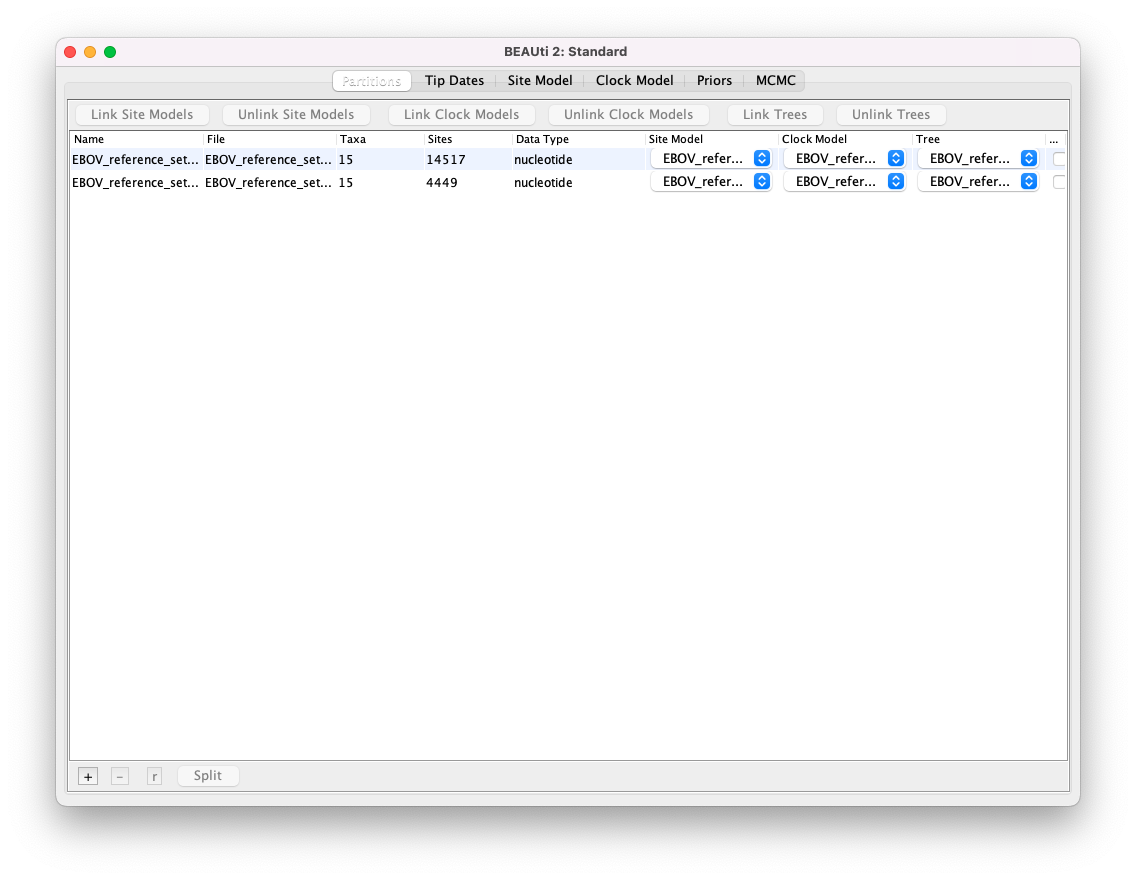
\includegraphics[max width=\textwidth, max height=0.9\textheight]{figures/data1.png}
    \caption{Data imported into BEAUti2.}
    \label{fig:data1}
\end{figure}

\subsubsection{Setting up partition models}\label{setting-up-partition-models}

A common way to account for site-to-site rate heterogeneity (variation
in substitution rates between different sites) is to use a Gamma site
model. In this model, we assume that rate variation follows a Gamma
distribution. To make the analysis tractable the Gamma distribution is
discretised into a small number of bins (usually 4-6). The mean of each
bin then acts as a multiplier for the overall substitution rate. The
transition probabilities are then calculated for each scaled
substitution rate. To calculate the likelihood for a site we marginalise
over all rates, i.e.
\textbf{P(data \textbar{} tree, substitution model)} is calculated under
each Gamma rate category and the results are averaged over
all rates. This is a handy approach if we suspect that some
sites are evolving faster than others but the precise position of these
sites in the alignment is unknown. We will look at Gamma site models 
later in this tutorial.

Another, more straightforward, way to account for site-to-site rate heterogeneity is to split
the alignment into explicit partitions, and specify an independent
substitution model for each partition. This is useful when we have a good 
\textit{a priori} intuition about which positions in the alignment have different
substitution rates from the rest. In our example, our alignment 
is already split into coding and non-coding regions, and we further split the
coding region into two partitions: 1st and 2nd, and 3rd codon positions. This is 
because most mutations at 3rd codon positions are synonymous and we therefore 
expect them to have a faster substitution rate than 1st and 2nd codon positions. 



\begin{framed}
  Select the \lstinline!EBOV_reference_set_15_cds! partition (alignment). It should be 
  the top partition in the \textbf{Partitions} tab. Next click on \textbf{Split} at the 
  bottom and select \lstinline!{1,2} + 3! to partition the alignment into two partitions:
    \begin{itemize}
      \item 1st and 2nd codon positions
      \item 3rd codon positions
    \end{itemize}
  Now select all three partitions (use \textbf{shift+click}) and click \textbf{Link Clock Models} 
  and \textbf{Link Trees}. 

  You can also look at the individual alignments
  for each partition by double-clicking on the partition under the \textbf{File} column.
\end{framed}

\begin{figure}
    \centering
    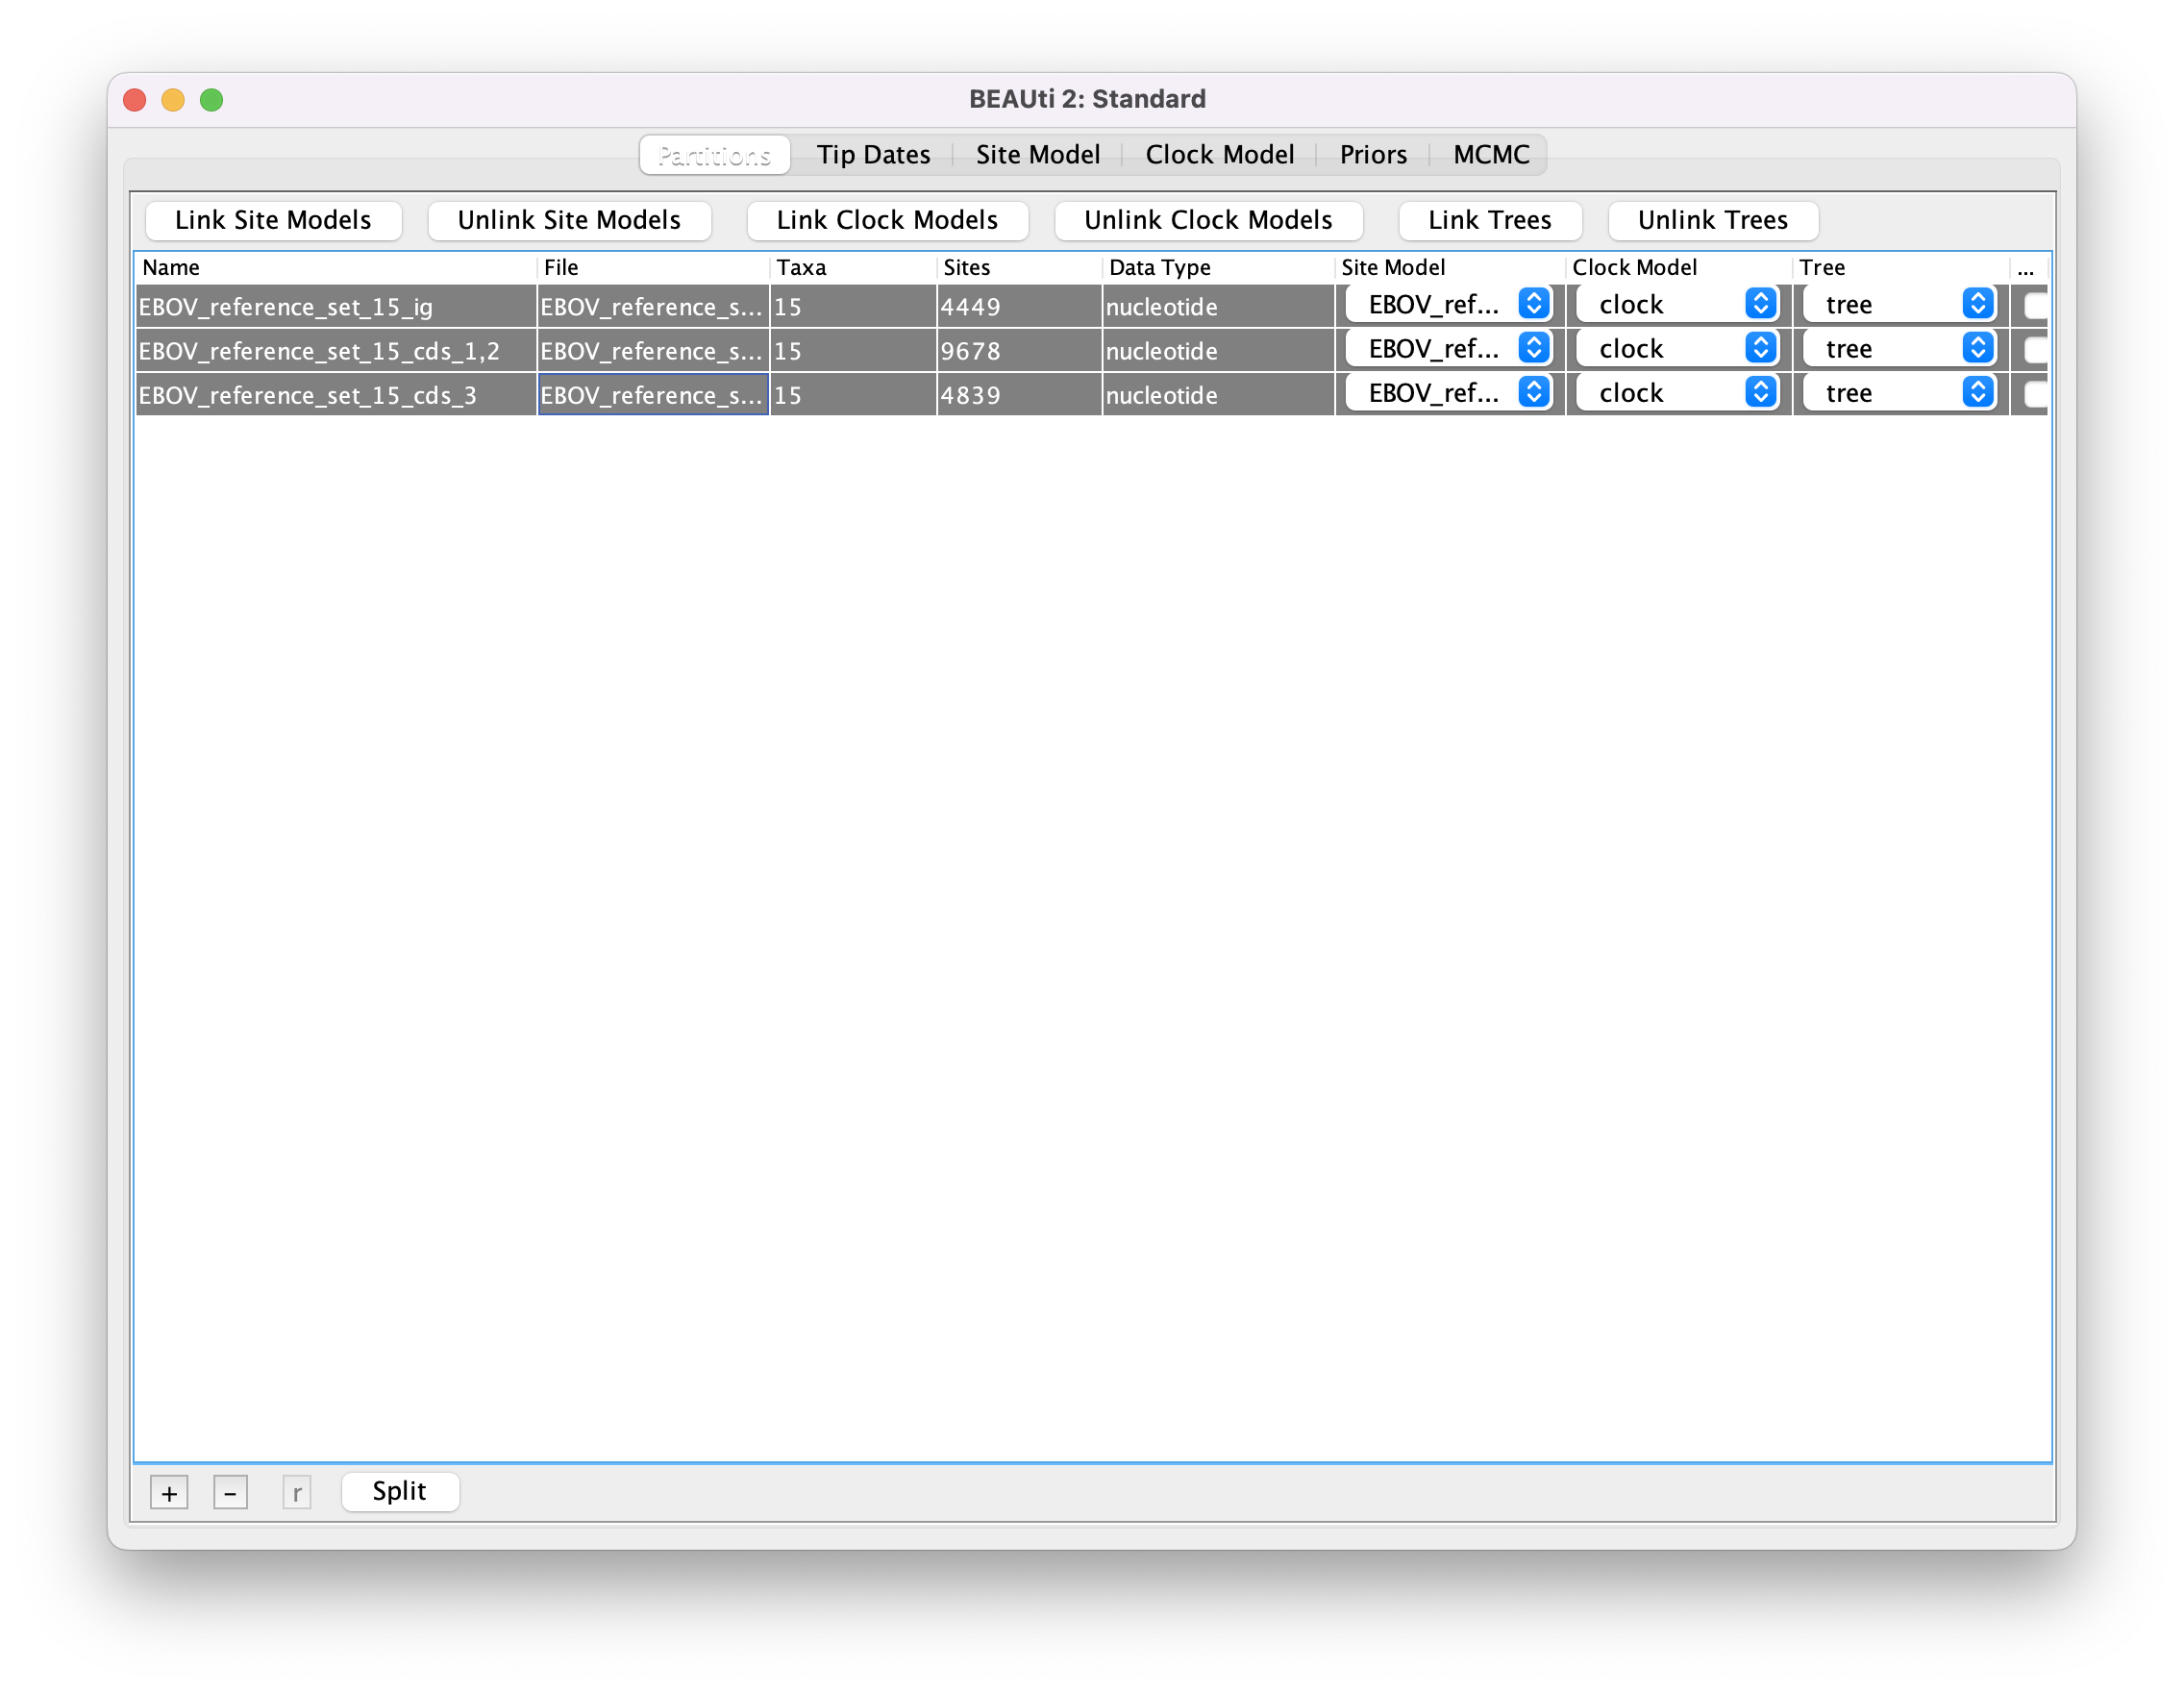
\includegraphics[max width=\textwidth, max height=0.9\textheight]{figures/data2.png}
    \caption{Partitioning the alignment and linking the clock and tree models.}
    \label{fig:data2}
\end{figure}

We linked trees and clock models, because by default BEAST2 would use
independent trees and clock models for each partition. There are cases 
(e.g. segmented viruses or when recombination is believed to play a large 
role) when we would not link the trees and clock models of different partitions. 

You will see that the \textbf{Clock Model} and the \textbf{Tree} columns
in the table both changed to \lstinline!EBOV_reference_set_15_ig!. Now we will
rename both models such that the following options and generated log
files are easier to read. The resulting setup should look as shown in
Figure \ref{fig:data2}.

\begin{framed}
Click on the first drop-down menu in the \textbf{Clock Model} column and
rename the shared clock model to \lstinline!clock!.

Likewise, rename the shared tree to \lstinline!tree!.
\end{framed}


\subsubsection{Setting the sampling dates}
The dataset contains genomes collected from outbreaks between 1976 and 2018. 
Since Ebola viruses evolve on the same timescale as the period over which 
the genomes were collected, we can use this information to calibrate the 
molecular clock. 

\begin{framed}
  In the \textbf{Tip Dates} panel, check the \textbf{Use tip dates} option
\end{framed}

The panel should now show the headers of the sequences in the Fasta file. Each
sequence header follows a regular format containing the Genbank identifier, 
sequence name, country of origin and collection date separated by vertical bars.

\begin{framed}
  In order for BEAST2 to use this information we must specify the format of the 
  date string and tell BEAST2 where to find the data. 
  \begin{itemize}
      \item Set \textbf{Dates specified} to the \lstinline!as dates with format! option. 
      \item Select \lstinline!yyyy-M-dd! from the dropdown box. 
      \item Click the \textbf{Auto-configure} button. A window will appear where you can specify how BEAUti can find the collection dates in the sequence headers (Figure~\ref{fig:tipdates}).
      \item Select \textbf{use everything} and specify \textbf{after last \textbar{}} and click \textbf{OK}.
  \end{itemize}
\end{framed}

\begin{figure}
    \centering
    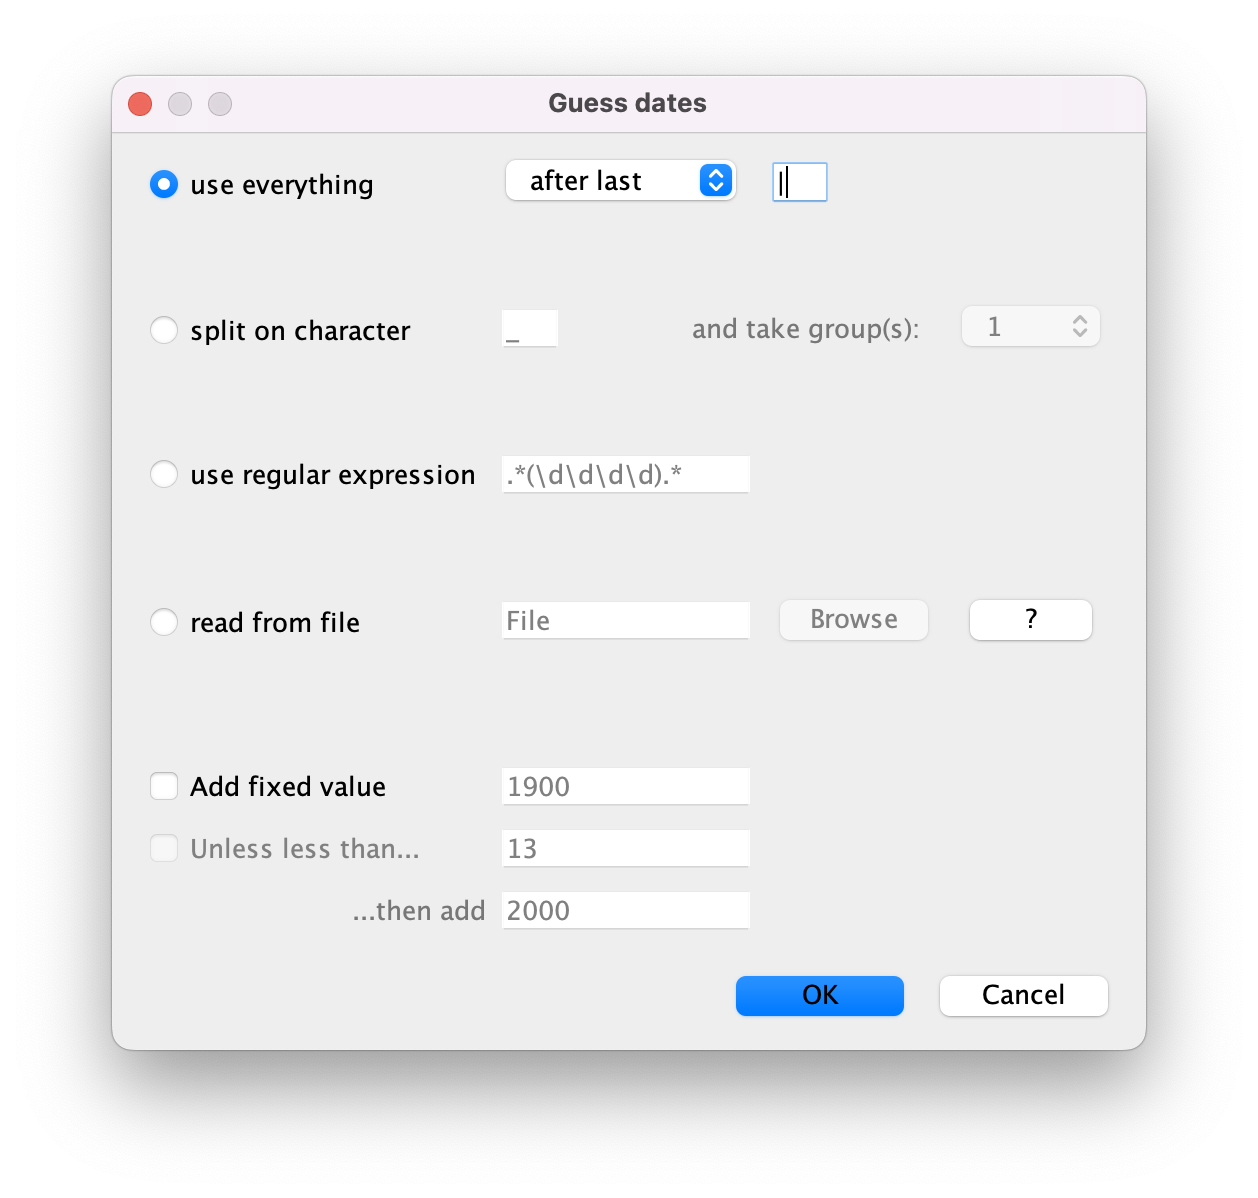
\includegraphics[max width=0.5\textwidth, max height=0.9\textheight]{figures/tipdates.png}
    \caption{Auto-configure tip dates.}
    \label{fig:tipdates}
\end{figure}

\begin{figure}
    \centering
    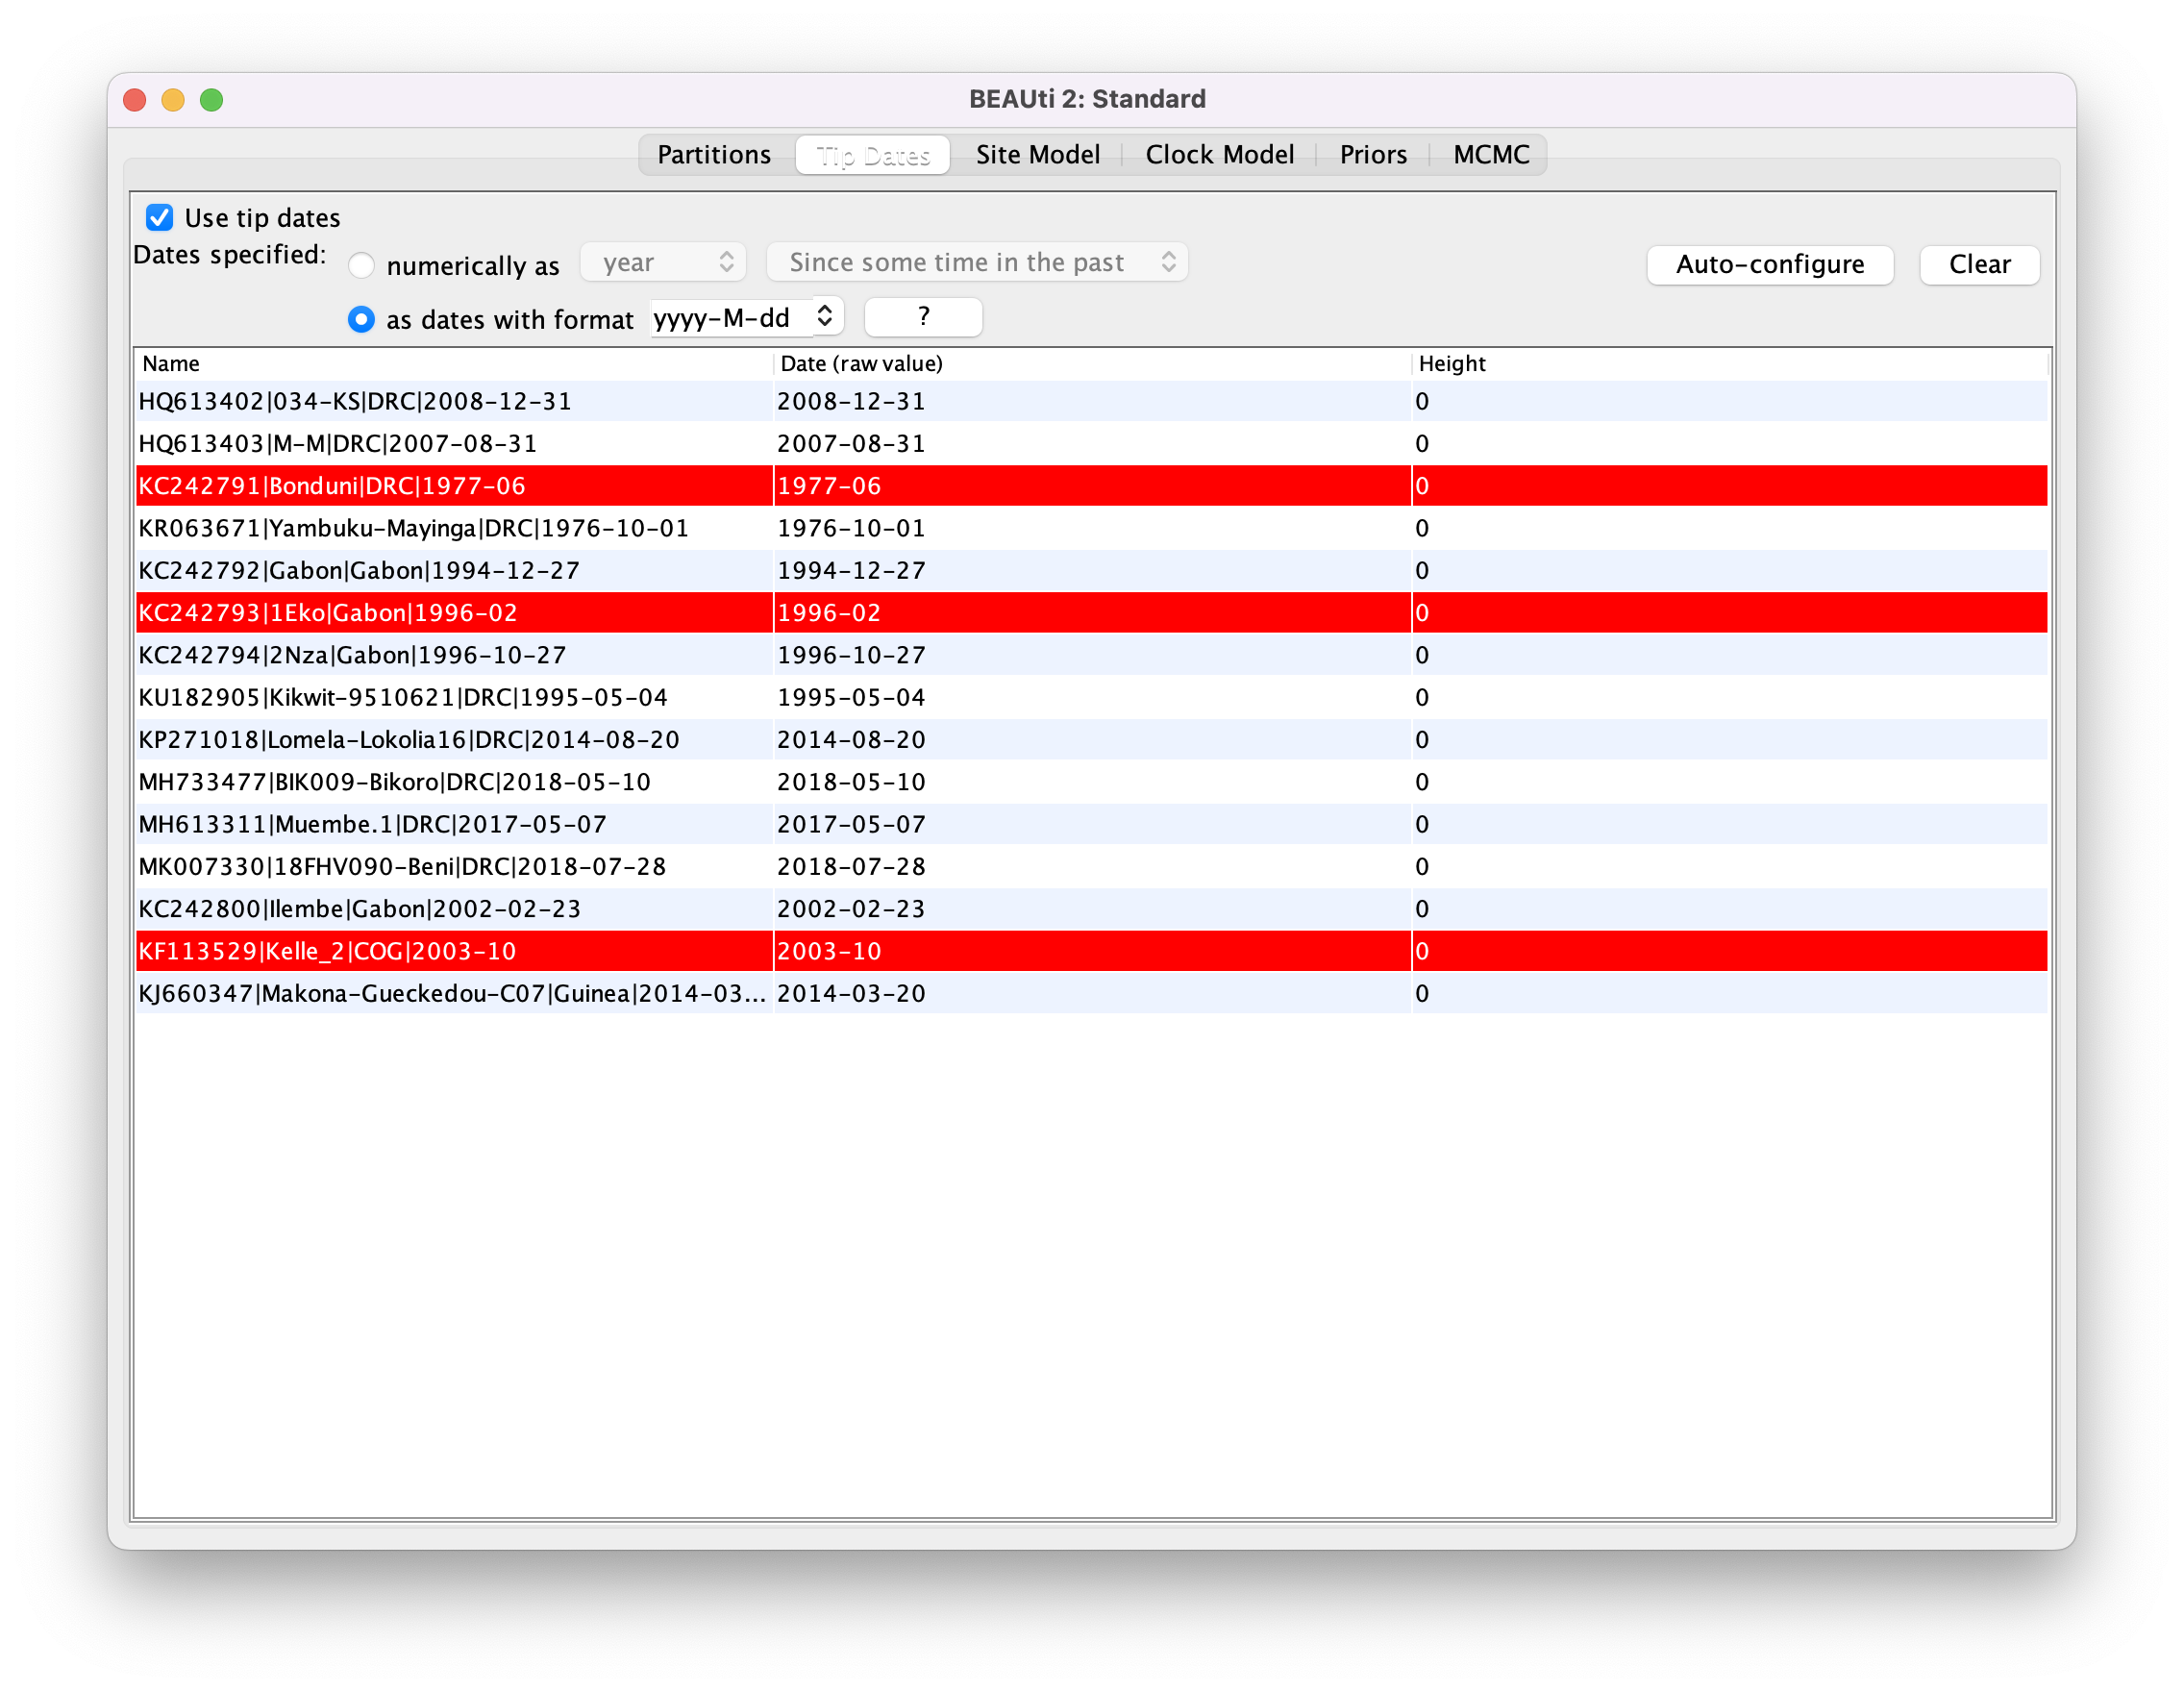
\includegraphics[max width=\textwidth, max height=0.9\textheight]{figures/parsingerror.png}
    \caption{Error parsing these collection dates!}
    \label{fig:parsingerror}
\end{figure}

This should throw a date parsing error and the panel should now look as in Figure~\ref{fig:parsingerror}. 
The collection dates for the three highlighted sequences could not be automatically parsed because they are only 
known up to the month and so don't follow the same format as the rest. To correct this we could edit the sequence headers in the Fasta files or we can simply manually edit the dates for these 3 sequences. Since we have no extra information we will use the middle of the month for the day. Alternatively we could enter the first day of the month. As the sequences in the dataset were collected over more than 40 years it is unlikely that a difference of less than 30 days will result in a big change to parameter estimates. Note that it is also possible to estimate the collection dates of sequences in BEAST2, but this cannot be set in BEAUti.

\begin{framed}
  Double-click on each of the red highlighted sequences under the \lstinline!Date (raw value)! column and 
  enter \textbf{15} as the day. Note that more errors will be thrown until all three dates are corrected! 
  When you're done the panel should look as in Figure~\ref{fig:datescorrected}.
\end{framed}


\begin{figure}
    \centering
    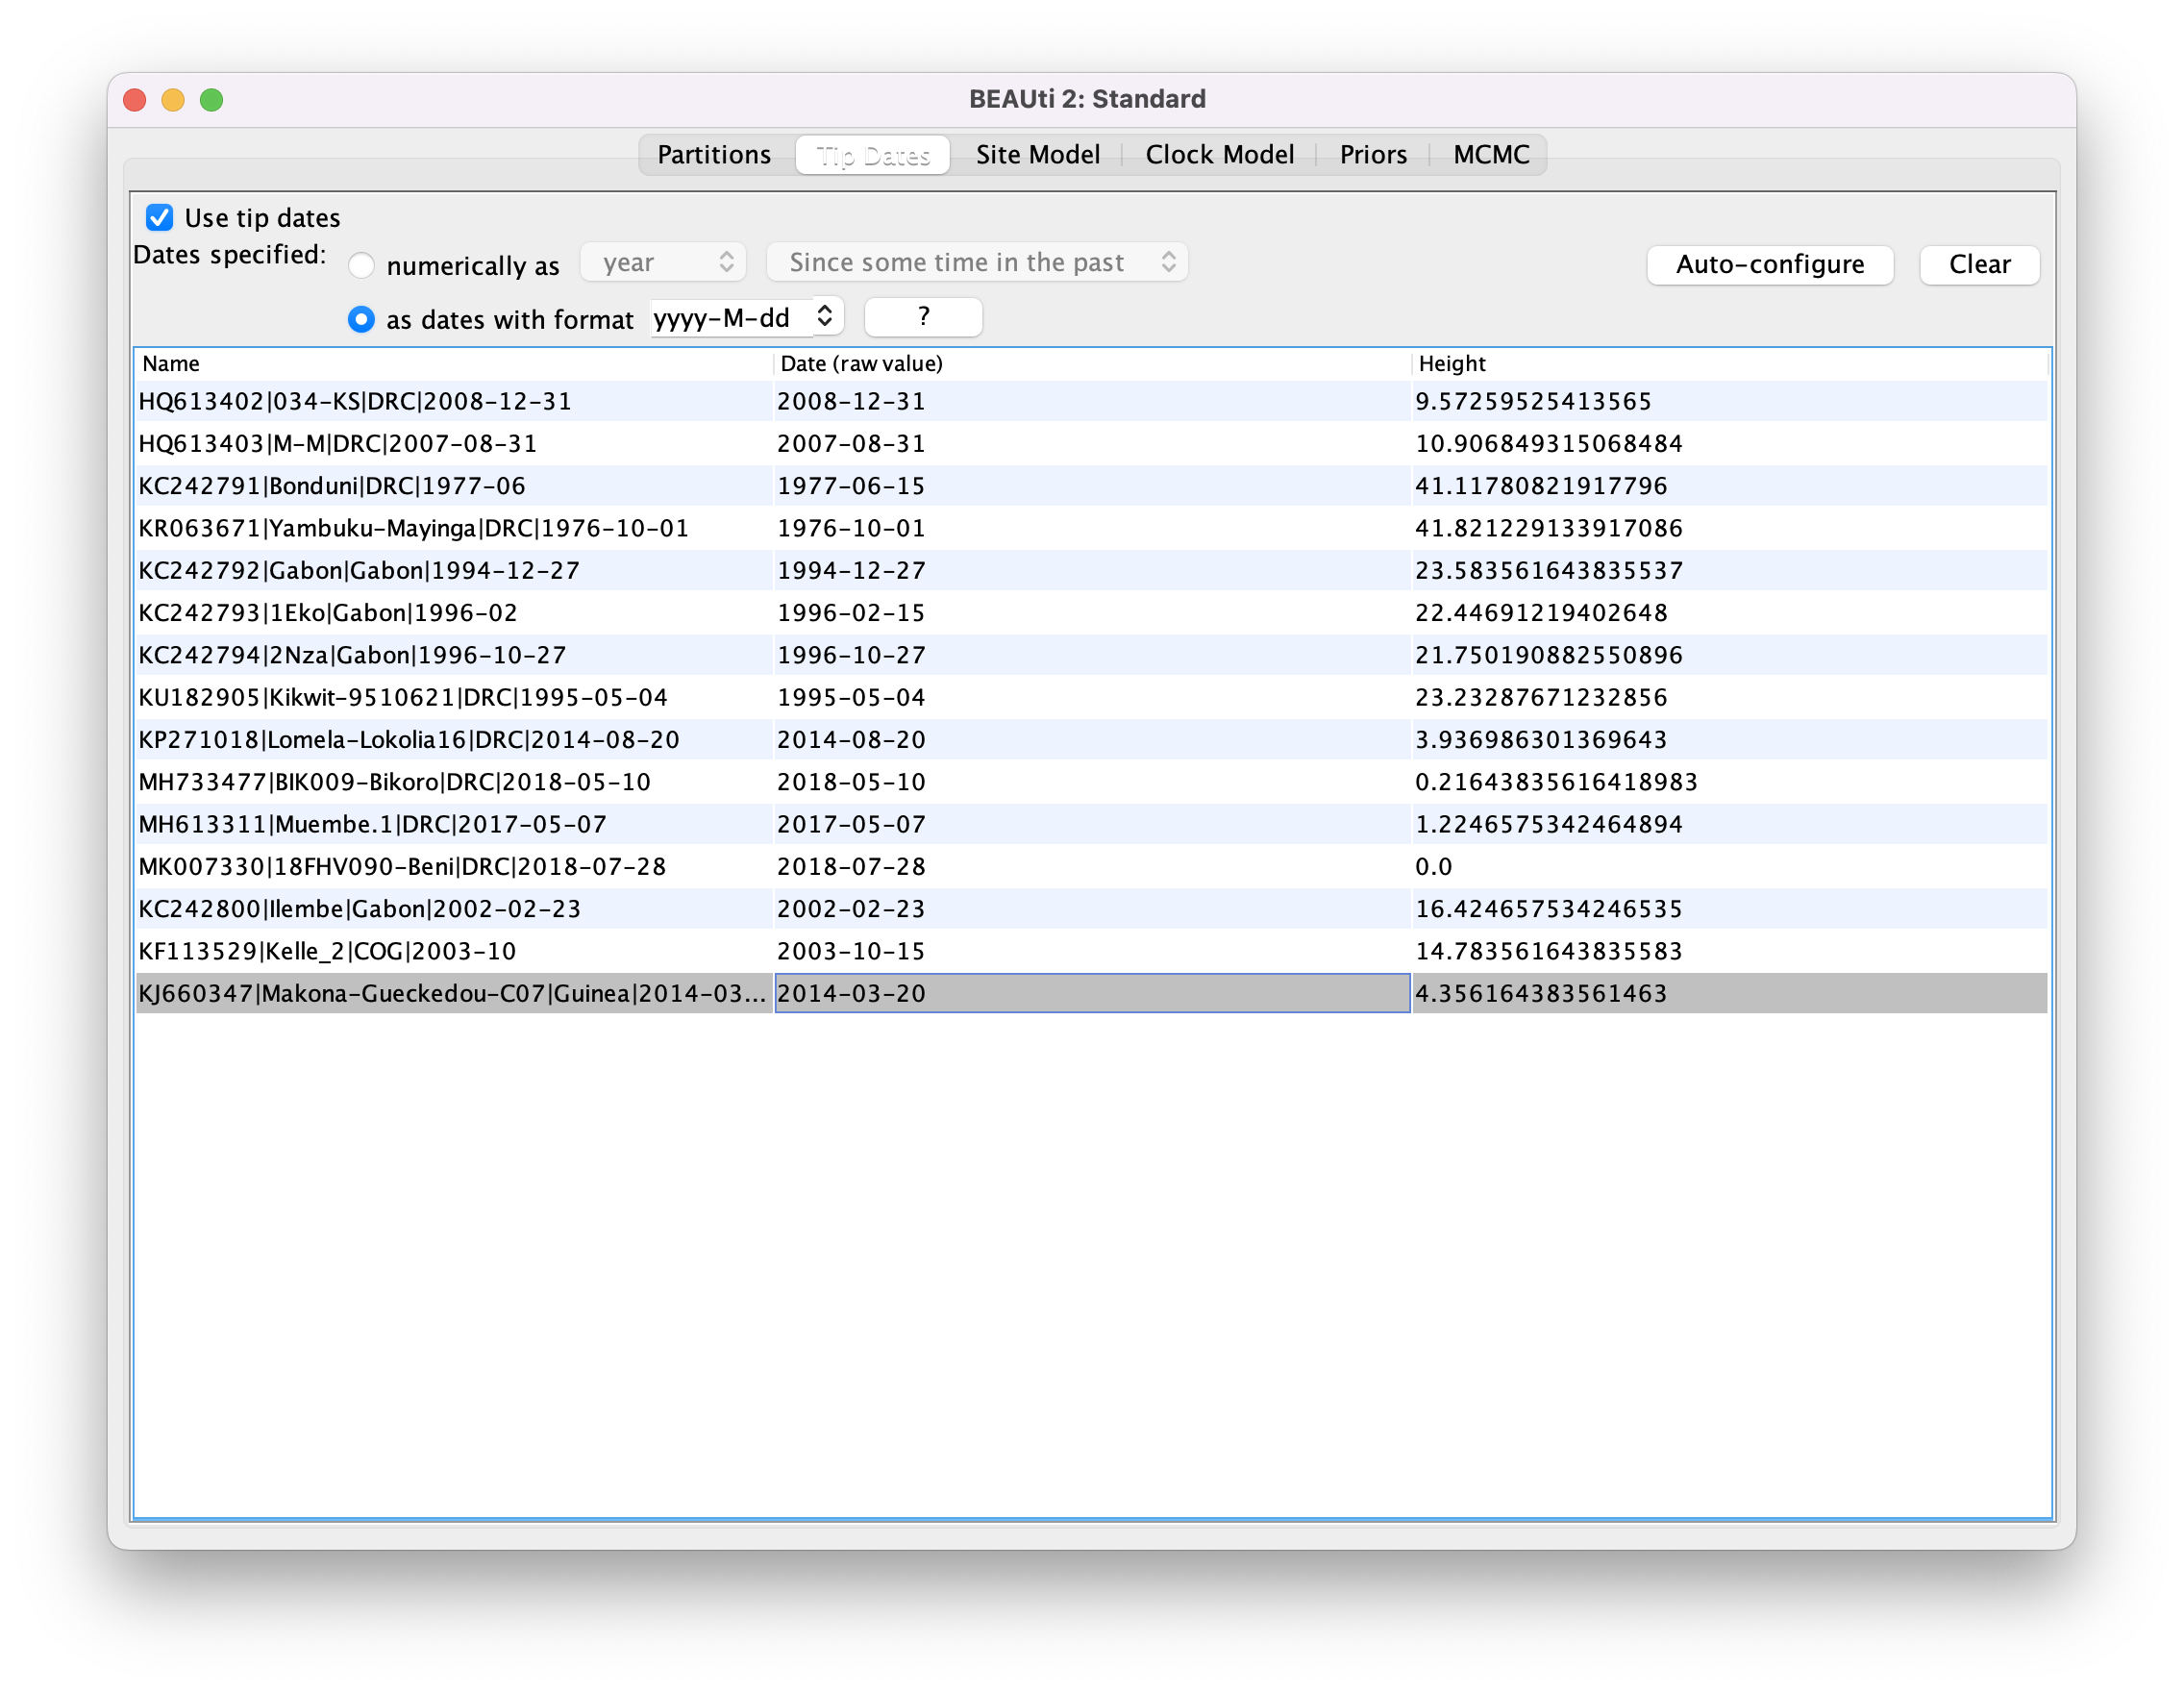
\includegraphics[max width=\textwidth, max height=0.9\textheight]{figures/datescorrected.png}
    \caption{Setting the tip dates.}
    \label{fig:datescorrected}
\end{figure}


\clearpage



\subsubsection{Setting up the substitution
model}\label{setting-the-substitution-model}

Next, we need to set up the substitution models for each partition in the \textbf{Site Model} tab.

\begin{framed}
Select the \textbf{Site Model} tab.
\end{framed}

The options available in this panel depend on whether the alignment data
are in nucleotides, amino-acids, binary data or general data. The
settings available after loading the alignment will contain the default
values which we normally want to modify.

The panel on the left shows each partition. Remember that we did not
link the substitution models in the previous step for the different
partitions, so each partition evolves under a different substitution
model, i.e.~we assume that different positions in the alignment
accumulate substitutions differently. We will need to set the site
substitution model separately for each part of the alignment as these
models are unlinked. However, we think that all partitions evolve
according to the same model (but with different parameter values).

\begin{framed}
Make sure that \lstinline!EBOV_reference_set_15_ig! is selected.

\begin{itemize}

\item
  Check the \textbf{estimate} checkbox for \textbf{Substitution Rate}.
\item
  Select \textbf{HKY} in the \textbf{Subst Model} drop-down menu.
\item
  Select \textbf{Empirical} from the \textbf{Frequencies} drop-down
  menu.
\end{itemize}

Note that when you checked \textbf{estimate} for the substitution rate a
yellow circle with a cross appeared to the right of \textbf{Fix mean
substitution rate}. If you hover your cursor above the circle you will
see a warning. \textbf{Ignore} the warning and continue with the next
step.
\end{framed}

\begin{figure}
    \centering
    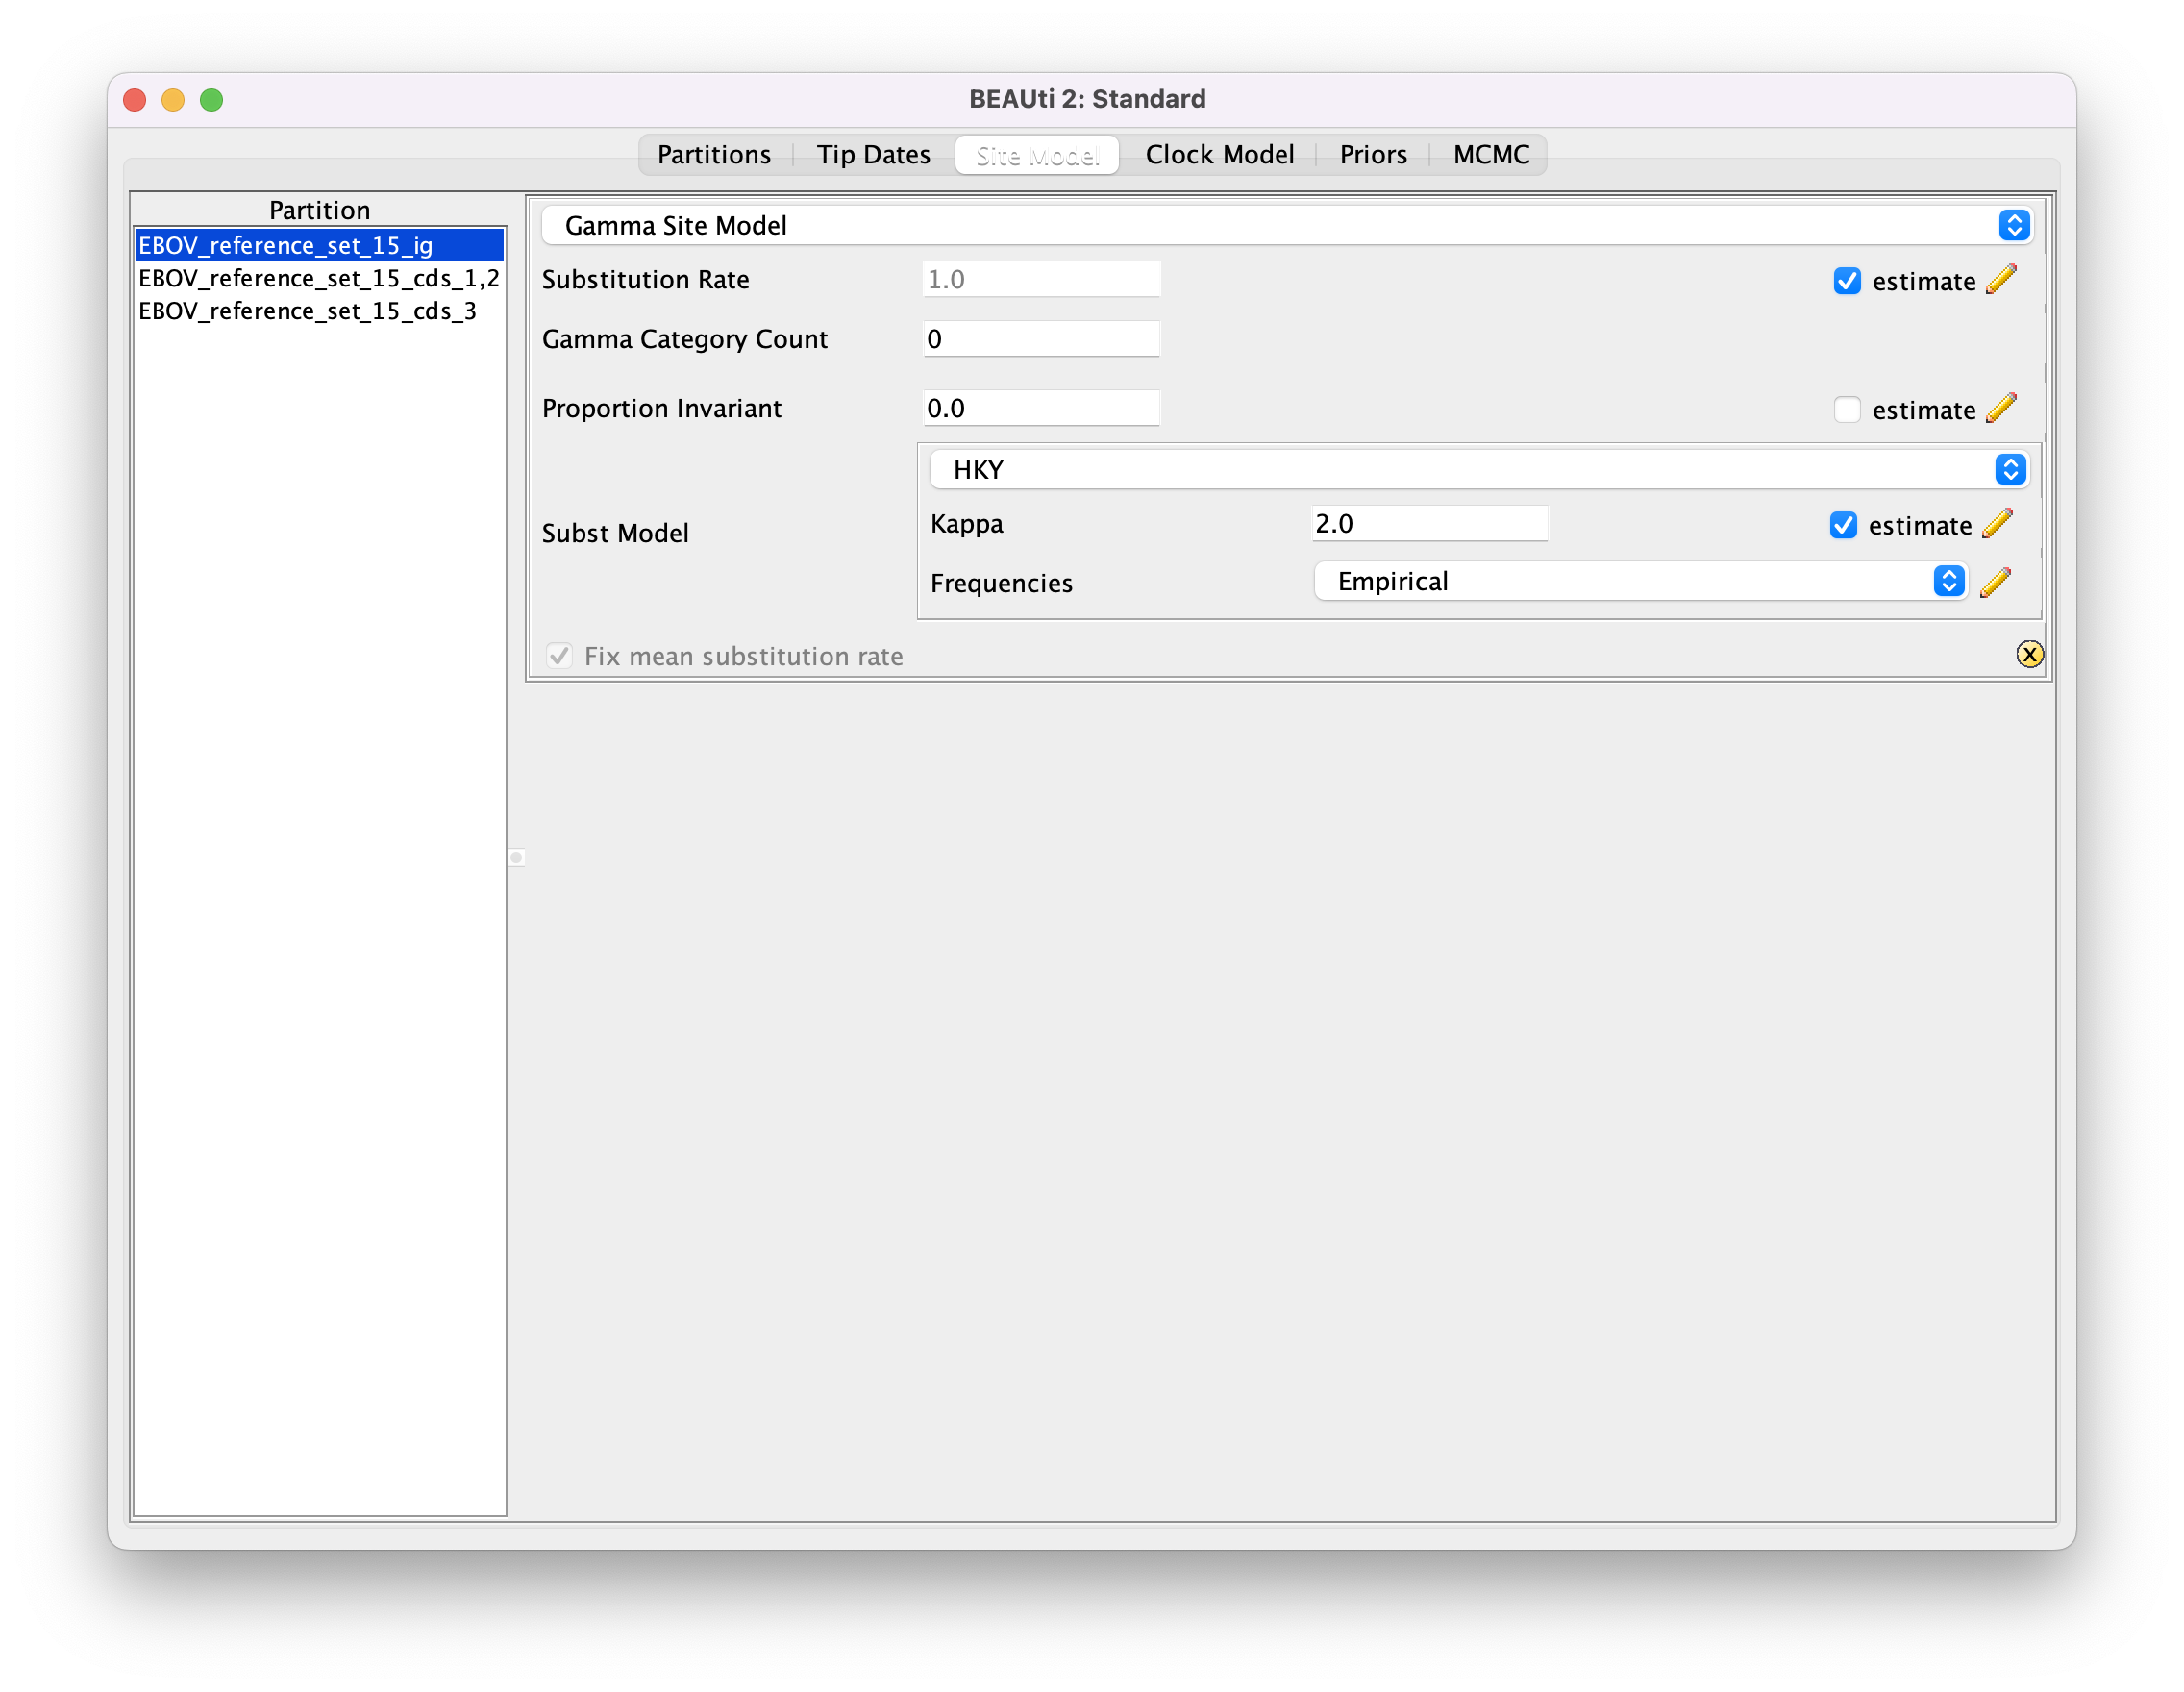
\includegraphics[max width=\textwidth, max height=0.9\textheight]{figures/substitution.png}
    \caption{Site model setup.}
    \label{fig:subst}
\end{figure}

The panel should look like in Figure~\ref{fig:subst}.

We are using an HKY substitution model with empirical frequencies. This
will fix the frequencies to the proportions observed in the partition.
This approach means that we can get a good fit to the data without
explicitly estimating these parameters. Next we \emph{could} repeat the above 
steps for each of the remaining partitions or we can take a shortcut.

\begin{framed}
Select the remaining two partitions (use \textbf{shift+click}). The
window will now look like Figure \ref{fig:clone}.

Click \textbf{OK} to to clone the site model for the other three
partitions from \lstinline!EBOV_reference_set_15_ig!.
\end{framed}

\begin{figure}
    \centering
    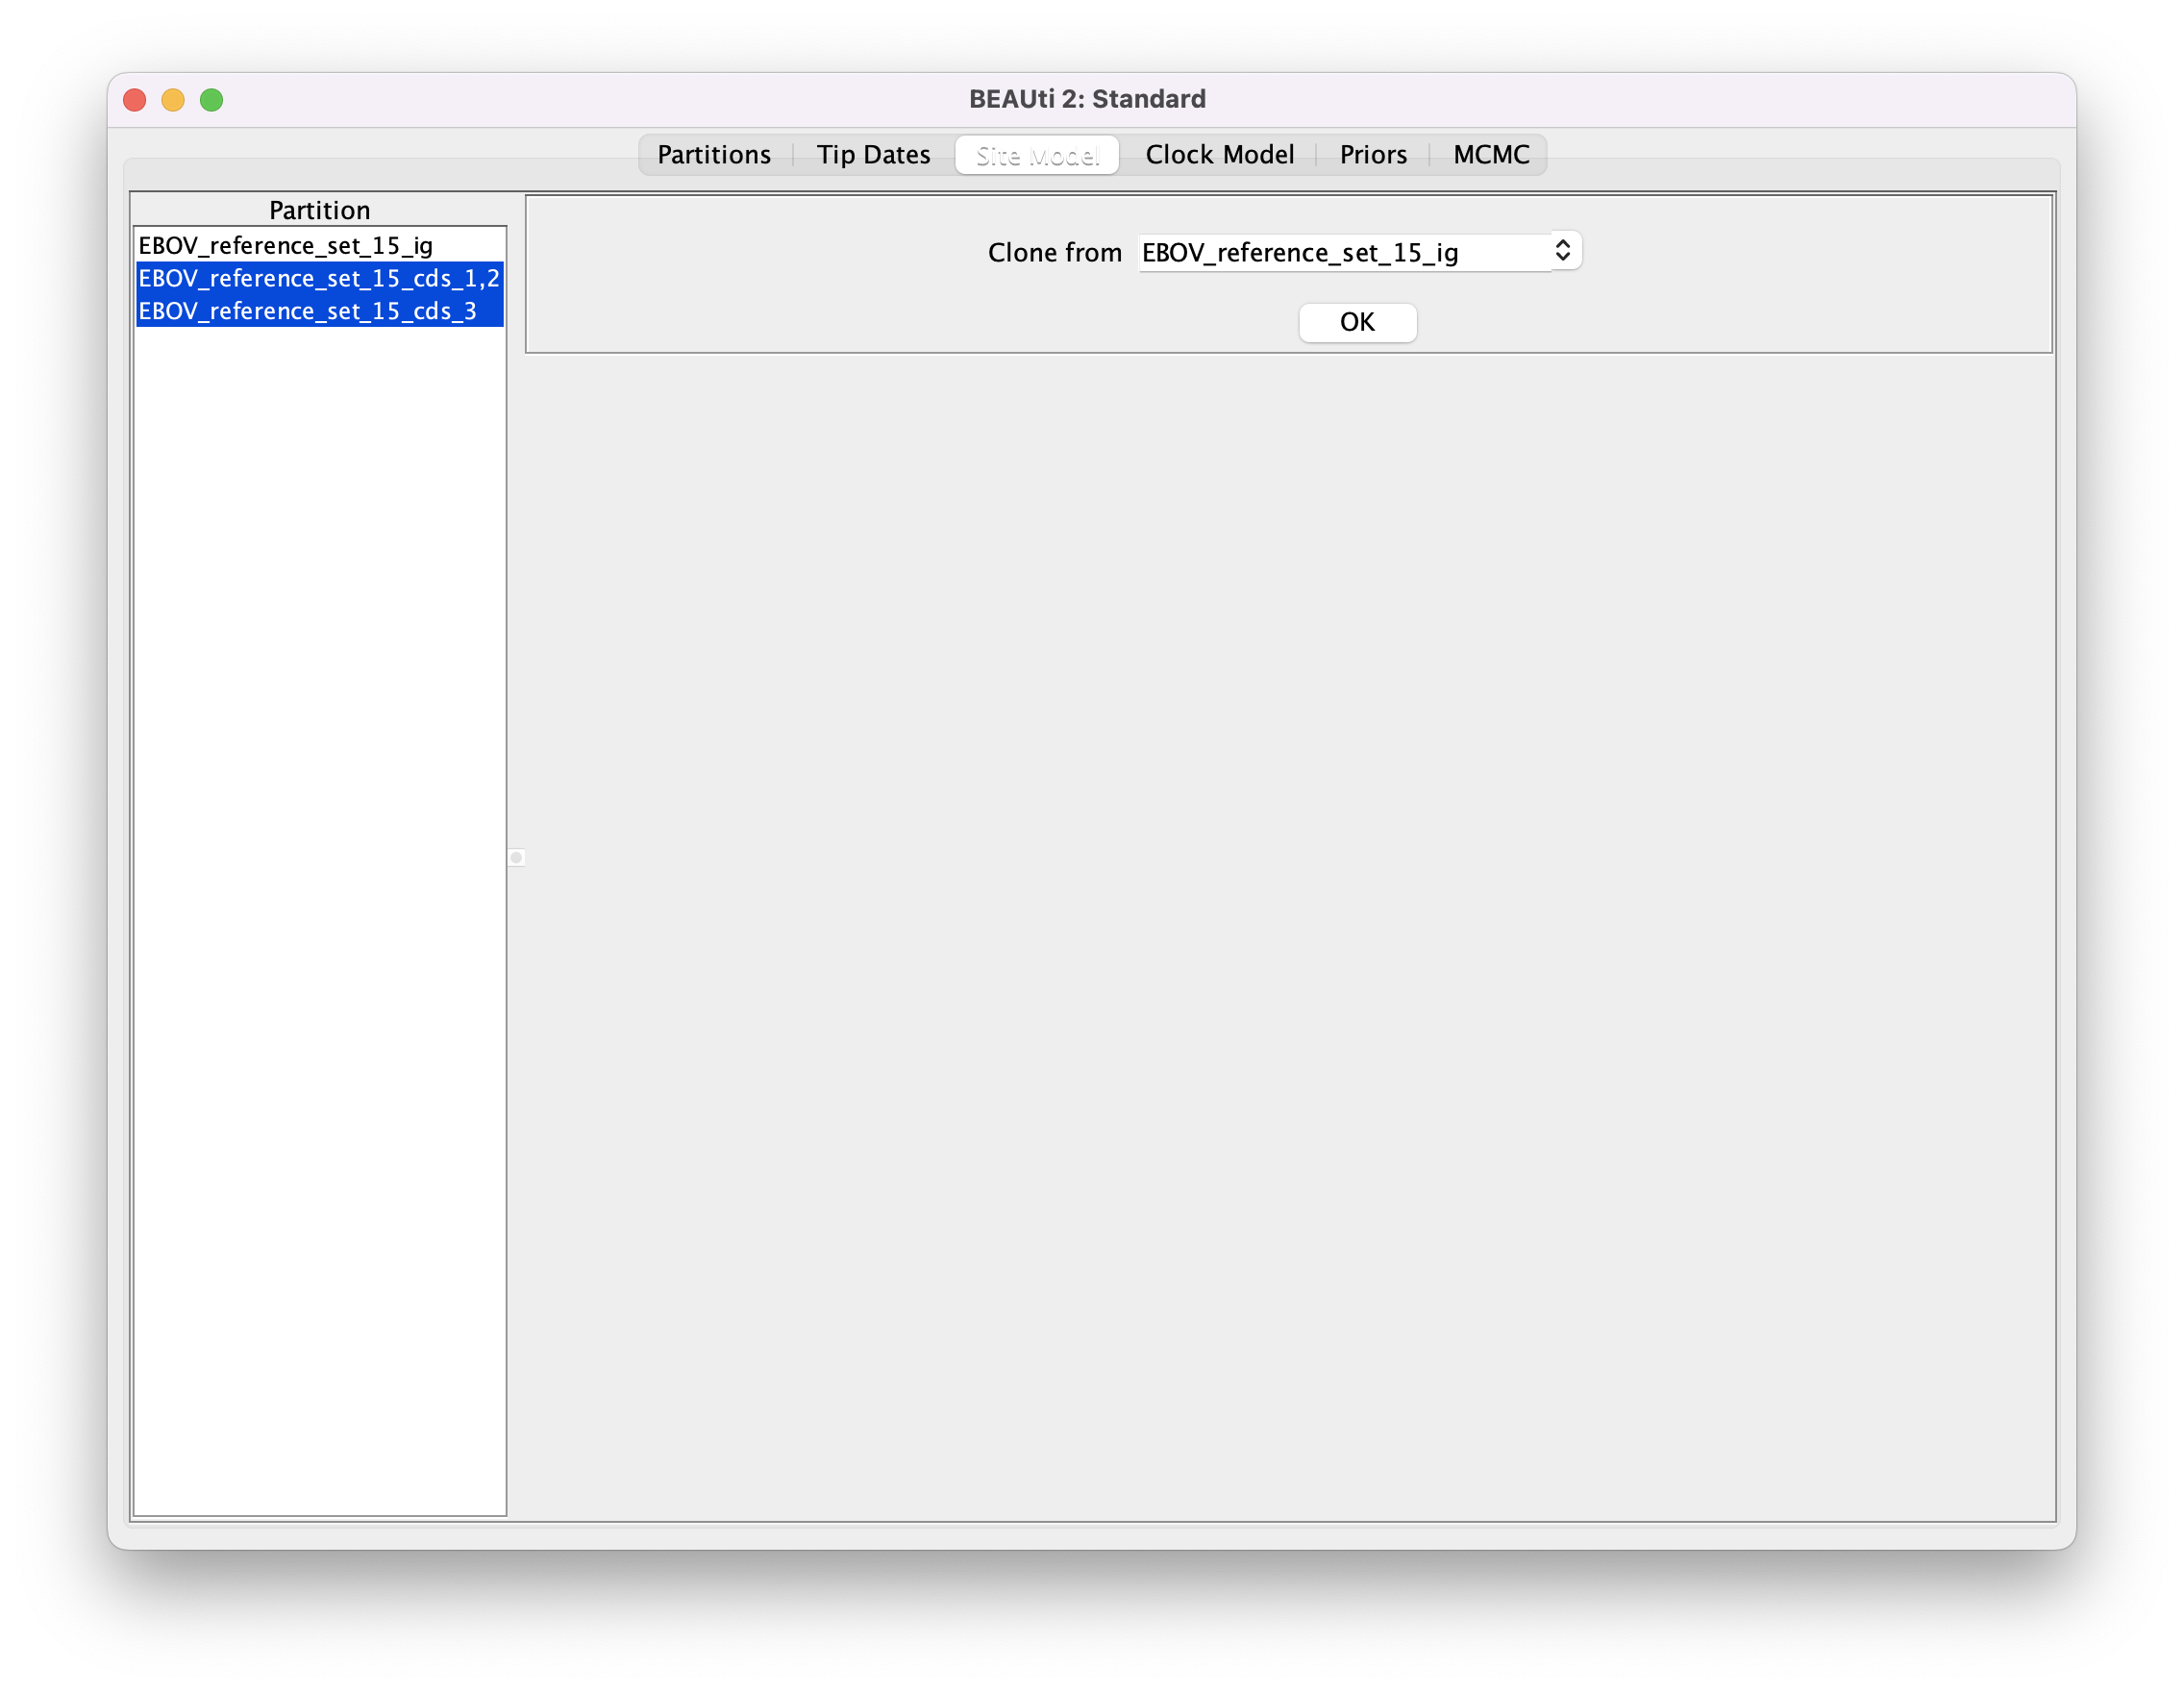
\includegraphics[max width=\textwidth, max height=0.9\textheight]{figures/clone.png}
    \caption{Shortcut to clone site models between partitions.}
    \label{fig:clone}
\end{figure}

If you did everything correctly the yellow circle with a cross to the
right of \textbf{Fix mean substitution rate} should have disappeared.

\begin{framed}
\textbf{Topic for discussion:} Can you figure out the reason for the
warning when you checked \textbf{estimate} for the substitution rate?
Don't worry if you can't figure it out, the reason for the warning is
explained in detail in later tutorials.
\end{framed}




\subsubsection{Setting the clock model}\label{setting-the-clock-model}

Next, select the \textbf{Clock Model} tab at the top of the main window.
This is where we set up the molecular clock model. For this initial analysis we
are going to leave the selection at the default value of a strict
molecular clock, which assumes a steady linear accummulation of mutations over
time, with no variation among branches in the tree. 

\begin{framed}
Click on the \textbf{Clock Models} tab and view the setup \emph{(but
don't do anything)}.
\end{framed}

\subsubsection{Setting priors}\label{setting-priors}

The \textbf{Priors} tab allows prior distributions to be specified for
each model parameter. The model selections made in the \textbf{Site
Model} and \textbf{Clock Model} tabs determine which parameters are
included in the model. For each of these parameters a prior distribution
needs to be specified. It is also possible to specify hyperpriors (and
hyper-hyperpriors etc.) for each of the model parameters. We also need
to specify a prior for the \textbf{Tree} that describes the prior 
expectation for how the tree grows over time. 

In this example we use a basic Kingman coalescent model for the tree prior. 
This simple model assumes a constant effective population size through time. 
This makes sense for our scenario, as we are modelling the virus within its
reservoir species (since we are only including one representative genome per outbreak
and we believe each outbreak was started by a single spillover from the reservoir).
As we believe the virus to be endemic in the reservoir we would expect the 
effective population size to remain constant over time.


\begin{framed}
Go to the \textbf{Priors} tab and select \textbf{Coalescent Constant Population}
in the drop-down menu next to \textbf{Tree.t:tree}.
\end{framed}

The \textbf{popSize} parameter measures the effective population size of 
the virus. We will leave its prior at the default one-on-X ($\frac{1}{X}$) prior.

By default there is a Uniform prior on the \textbf{clockRate} parameter of
the clock model, between $0$ and $\infty$. This is a very bad idea for 
a clock rate prior, because molecular clock rates are in general very small. 
Thus, we would want to change this prior to a distribution that places 
more weight on biologically realistic values. We know from human EBOV 
outbreaks that the molecular clock rate is approximately $1 \times 10^{-3}$ 
substitutions per site per year (s/s/y). However, the rate can be elevated during
an exponentially growing human outbreak and we expect the long-term substitution
rate in the animal reservoir would likely be a little slower. 

\begin{framed}
For \textbf{clockRate.c:clock} select \textbf{Log Normal} from the drop-down
menu

\begin{itemize}

\item
  Expand the options for \textbf{clockRate.c:clock} using the arrow
  button on the left.
\item
  Set the \textbf{M} parameter to \textbf{1E-3}.
\item
  Set the \textbf{S} parameter to \textbf{0.5}
\item
  Check the \textbf{Mean in Real Space} box
\end{itemize}
\end{framed}


Note that BEAUti displays a plot of the prior distribution on the right,
as well as a few of its quantiles. This is for easy reference and can
help us to decide if a prior is appropriate. The lognormal prior
we are using is defined on $ (0,\infty) $ and would easily allow the rate to 
be slower than $1 \times 10^{-3}$ s/s/y, but would also penalise much faster
and biologically unrealistic rates.

If we wanted to add a hyperprior on one of the parameters of the lognormal
prior we would check the \textbf{estimate} box on the right of the
parameter. We could also change the initial values or limits of the
model parameters by clicking on the boxes next to the drop-down menus.
Do \textbf{not} do this here, as we are \textbf{not} adding any
hyperpriors or changing limits in this analysis!

The only remaining model parameters are the transition-transversion ratios 
for the substitution models on each partition (the \textbf{kappa} parameters). 
If we had chosen to estimate the nucleotide frequencies there would also be 
priors for the frequency parameters.   
\textbf{We will leave the rest of the priors on their default values!}
The BEAUti panel should look as shown in Figure \ref{fig:priors}.

Please note that in general using default priors is frowned upon as
priors are meant to convey your prior knowledge of the parameters. It is
important to know what information the priors add to the MCMC analysis
and whether this fits your particular situation. In our case the default
priors are suitable for this particular analysis, however for further,
more complex analyses, we will require a clear idea of what the priors
mean. Getting this understanding is difficult and comes with experience.


\begin{figure}
    \centering
    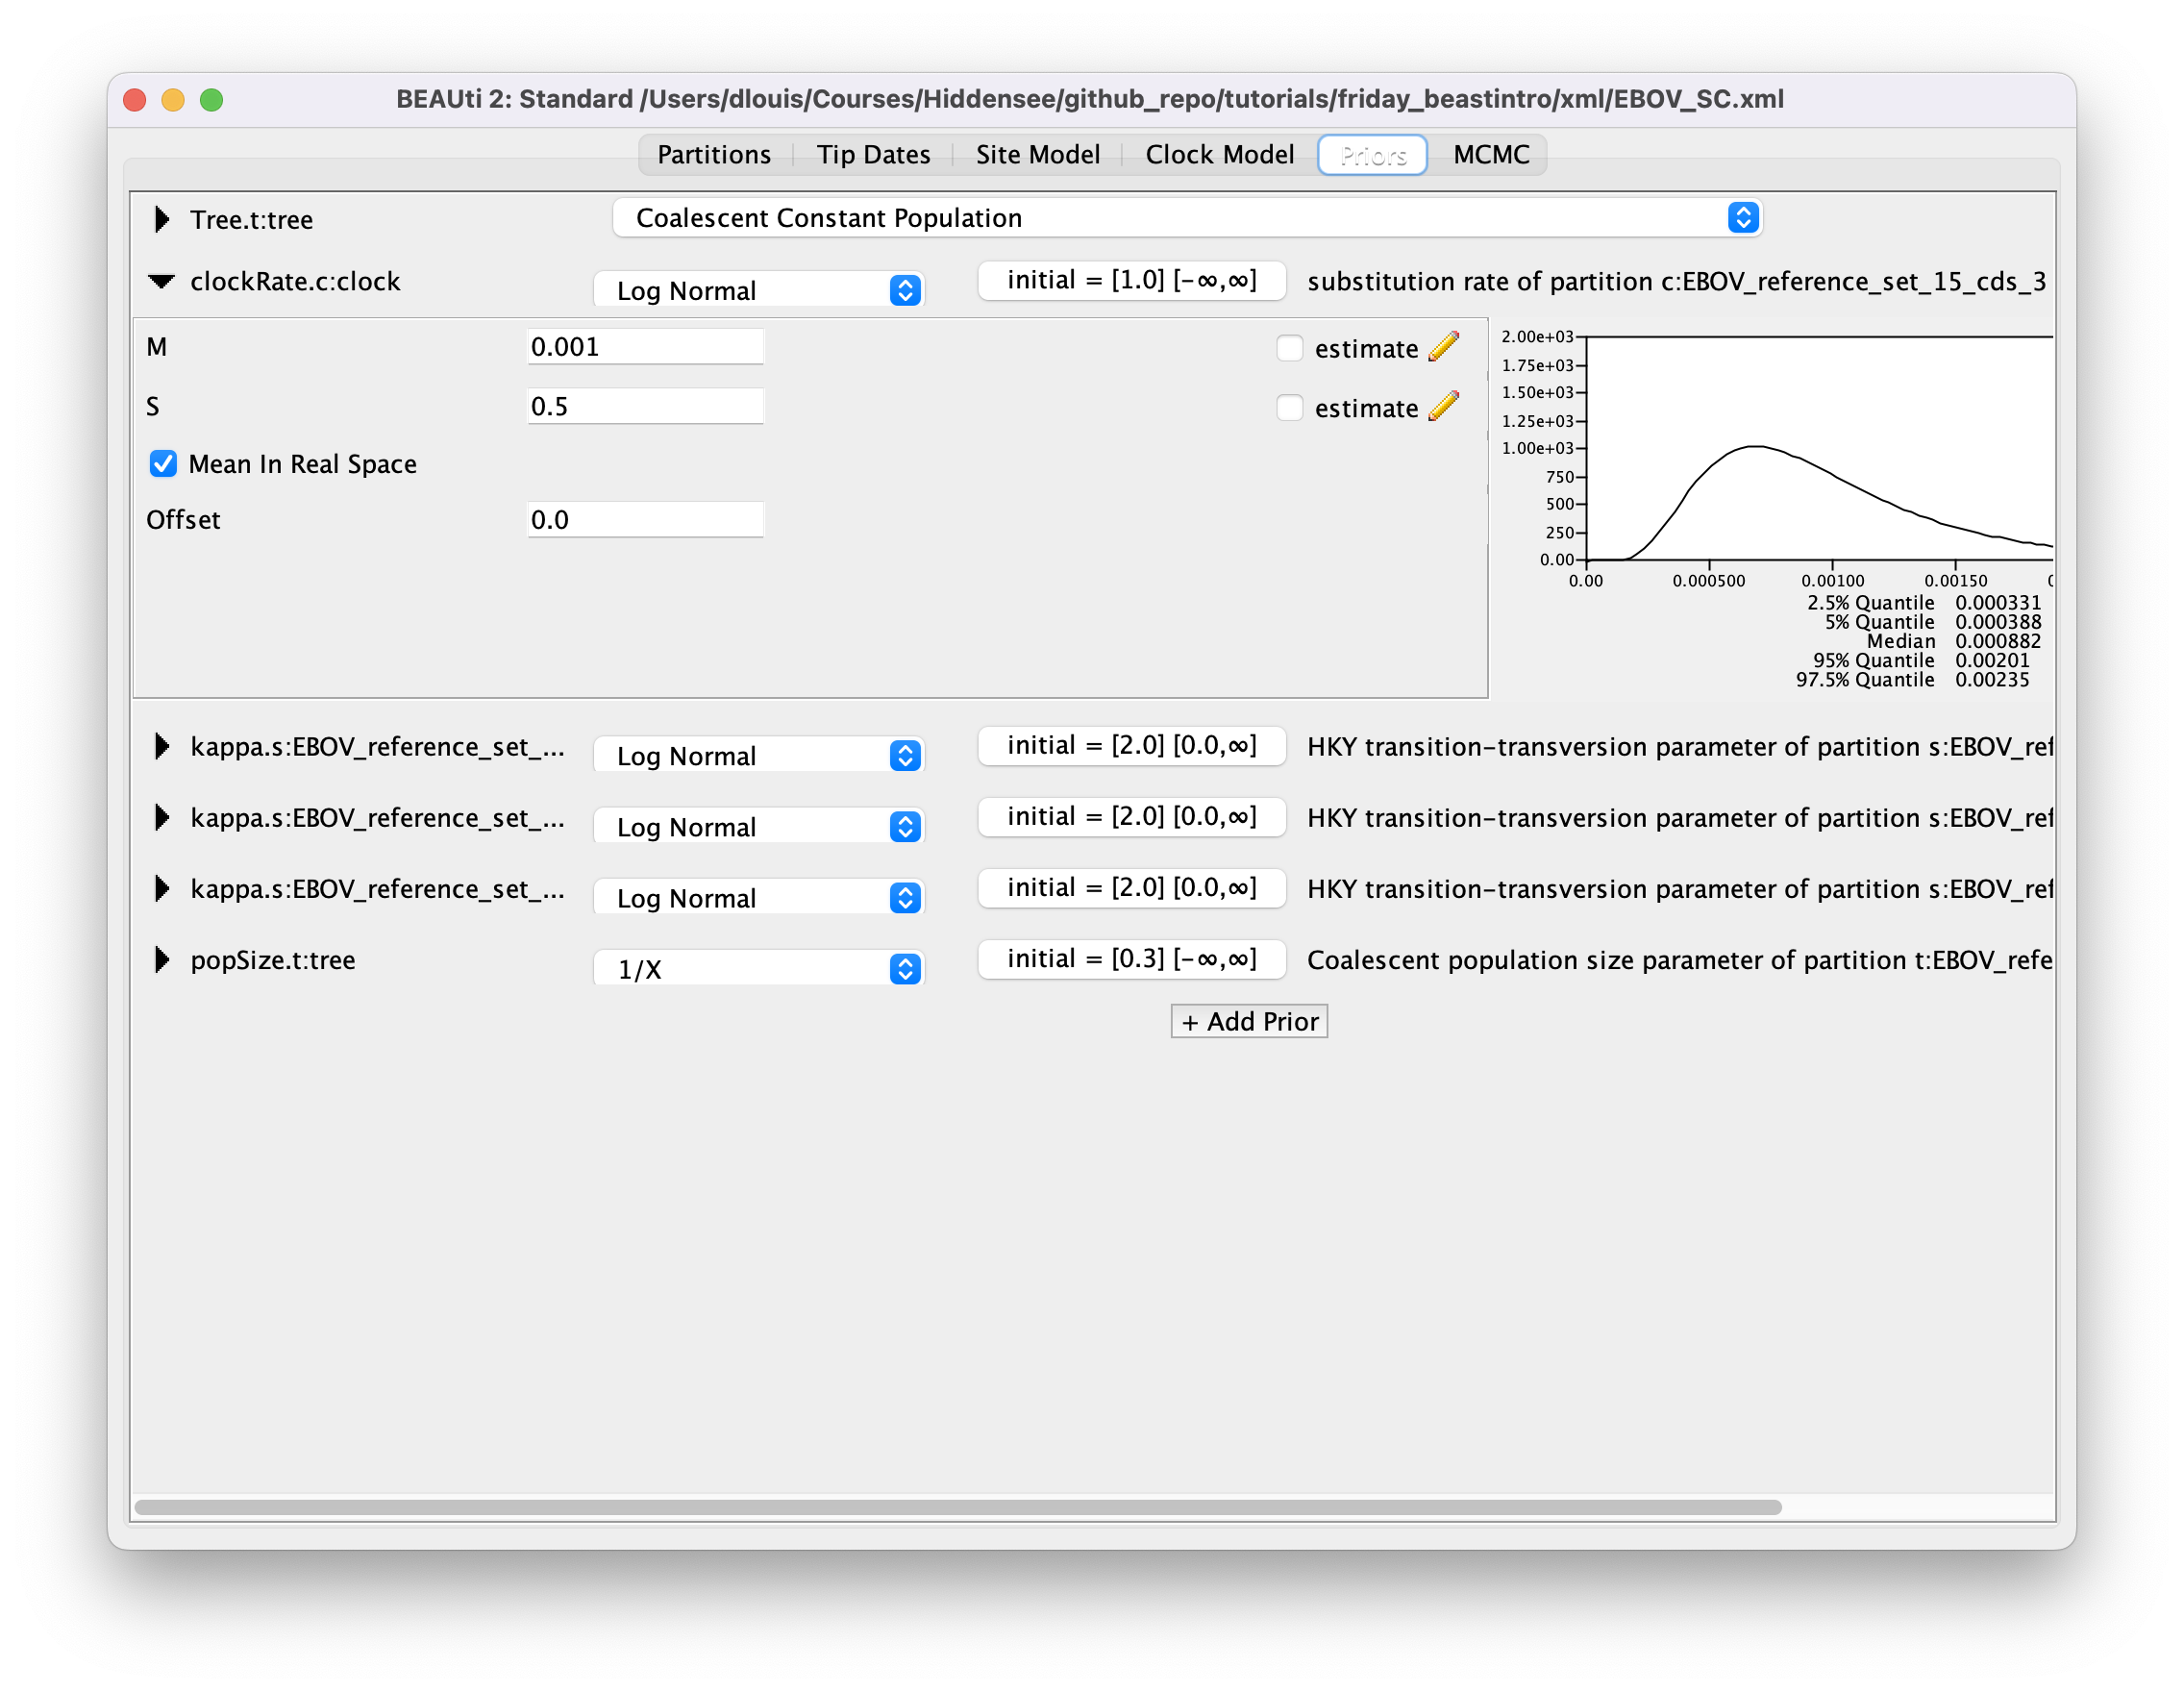
\includegraphics[max width=\textwidth, max height=0.9\textheight]{figures/priors.png}
    \caption{Prior setup.}
    \label{fig:priors}
\end{figure}



\subsubsection{Setting the MCMC options}\label{setting-the-mcmc-options}

Finally, the \textbf{MCMC} tab allows us to control the length of the MCMC
chain and the frequency of stored samples. It also allows one to change
the output file names.

\begin{framed}
Go to the \textbf{MCMC} tab.
\end{framed}

The \textbf{Chain Length} parameter specifies the number of steps the
MCMC chain will make before finishing (i.e.~the number of accepted
proposals). This number depends on the size of the dataset, the
complexity of the model and the precision of the answer required. The
default value of 10'000'000 is arbitrary and should be adjusted
accordingly. For this initial analysis we will leave the chain length as 
is, so that it will finish in a few minutes. We also leave the \textbf{Store Every}
and \textbf{Pre Burnin} fields at their default values.

Below these general settings you will find the logging settings. Each
particular option can be viewed in detail by clicking the arrow to the
left of it. You can control the names of the log files and how often
values will be stored in each of the files.

Start by expanding the \textbf{tracelog} options. This is the log file
you will use later to analyse and summarise the results of the run. The
\textbf{Log Every} parameter for the log file should be set relative to
the total length of the chain. Sampling too often will result in very
large files with little extra benefit in terms of the accuracy of the
analysis. Sampling too sparsely will mean that the log file will not
record sufficient information about the distributions of the parameters.
We normally want to aim to store no more than 10'000 samples so this
should be set to no less than chain length/10'000. 

\begin{framed}
Expand the \textbf{tracelog} options.

\begin{itemize}

\item
  Leave the \textbf{Log Every} parameter at \textbf{1000}.
\item
  Change the file name to \lstinline!EBOV_SC.log!
\end{itemize}
\end{framed}

Next, expand the \textbf{screenlog} options. The screen output is simply
for monitoring the program's progress. Since it is not so important,
especially if you run your analysis on a remote server or on a
cluster, the \textbf{Log Every} can be set to any value. However, if it
is set too small, the sheer quantity of information being displayed on
the screen will actually slow the program down. For this analysis we
will make BEAST2 log to screen every 10'000 samples, which will be easier
to follow than the default setting of every 1'000 samples.

\begin{framed}
Expand the \textbf{screenlog} options.

\begin{itemize}

\item
  Set the \textbf{Log Every} parameter to \textbf{10'000}
\end{itemize}
\end{framed}

Finally, we can also change the tree logging frequency by expanding
\textbf{treelog.t:tree}. For big trees with many taxa each individual
tree will already be quite large, thus if you log many trees the tree
files can easily become extremely large. You would be amazed at how
quickly BEAST can fill up even the biggest of drives if the tree logging
frequency is too high! For this reason it is often a good idea to set
the tree logging frequency lower than the trace log (especially for
analyses with many taxa). However, be careful, as the post-processing
steps of some models (such as the Bayesian skyline plot) require the
trace and tree logging frequencies to be identical!

\begin{framed}
Expand the \textbf{treelog.t:tree} options.

\begin{itemize}

\item
  Set the \textbf{File Name} to \lstinline!EBOV_SC.trees!.
\item
  Leave the \textbf{Log Every} parameter at the default value of 1'000.
\end{itemize}
\end{framed}


\subsubsection{Generating the XML file}\label{generating-the-xml-file}

We are now ready to create the BEAST2 XML file. This is the final
configuration file BEAST2 can use to execute the analysis.

\begin{framed}
Save the XML file under the name \lstinline!EBOV_SC.xml! using
\textbf{File \textgreater{} Save}.
\end{framed}

Do \textbf{NOT} close BEAUti, as we will return to it in the following sections!

\clearpage

\subsection{Running the analysis}\label{running-the-analysis}

Now open BEAST2 and provide your newly created XML file as input. You can
also change the \textbf{random number seed} for the run. This number is
the starting point of a pseudo-random number chain BEAST2 will use to
generate the samples. As computers are unable to generate truly random
numbers, we have to resort to generating deterministic sequences of
numbers that only look random, but will be identical when the starting
seed is the same. If your MCMC run converges to the true posterior then
you will be able to draw the same conclusions regardless of which random
seed is provided. However, if you want to exactly reproduce the results
of a run you need to start it with the same random number seed. For the 
results below we used the random seed 777.

\begin{framed}
Run the \textbf{BEAST2} program.

\begin{itemize}

\item
  Select \lstinline!EBOV_SC.xml! as the \textbf{Beast XML File}.
\item
  Set the \textbf{Random number seed} to \textbf{777} (or pick your
  favourite number).
\item
  Check the \textbf{Use BEAGLE library if available} checkbox. If you
  have previously installed BEAGLE this will make the analysis run
  faster.
\end{itemize}
\end{framed}

\begin{figure}
    \centering
    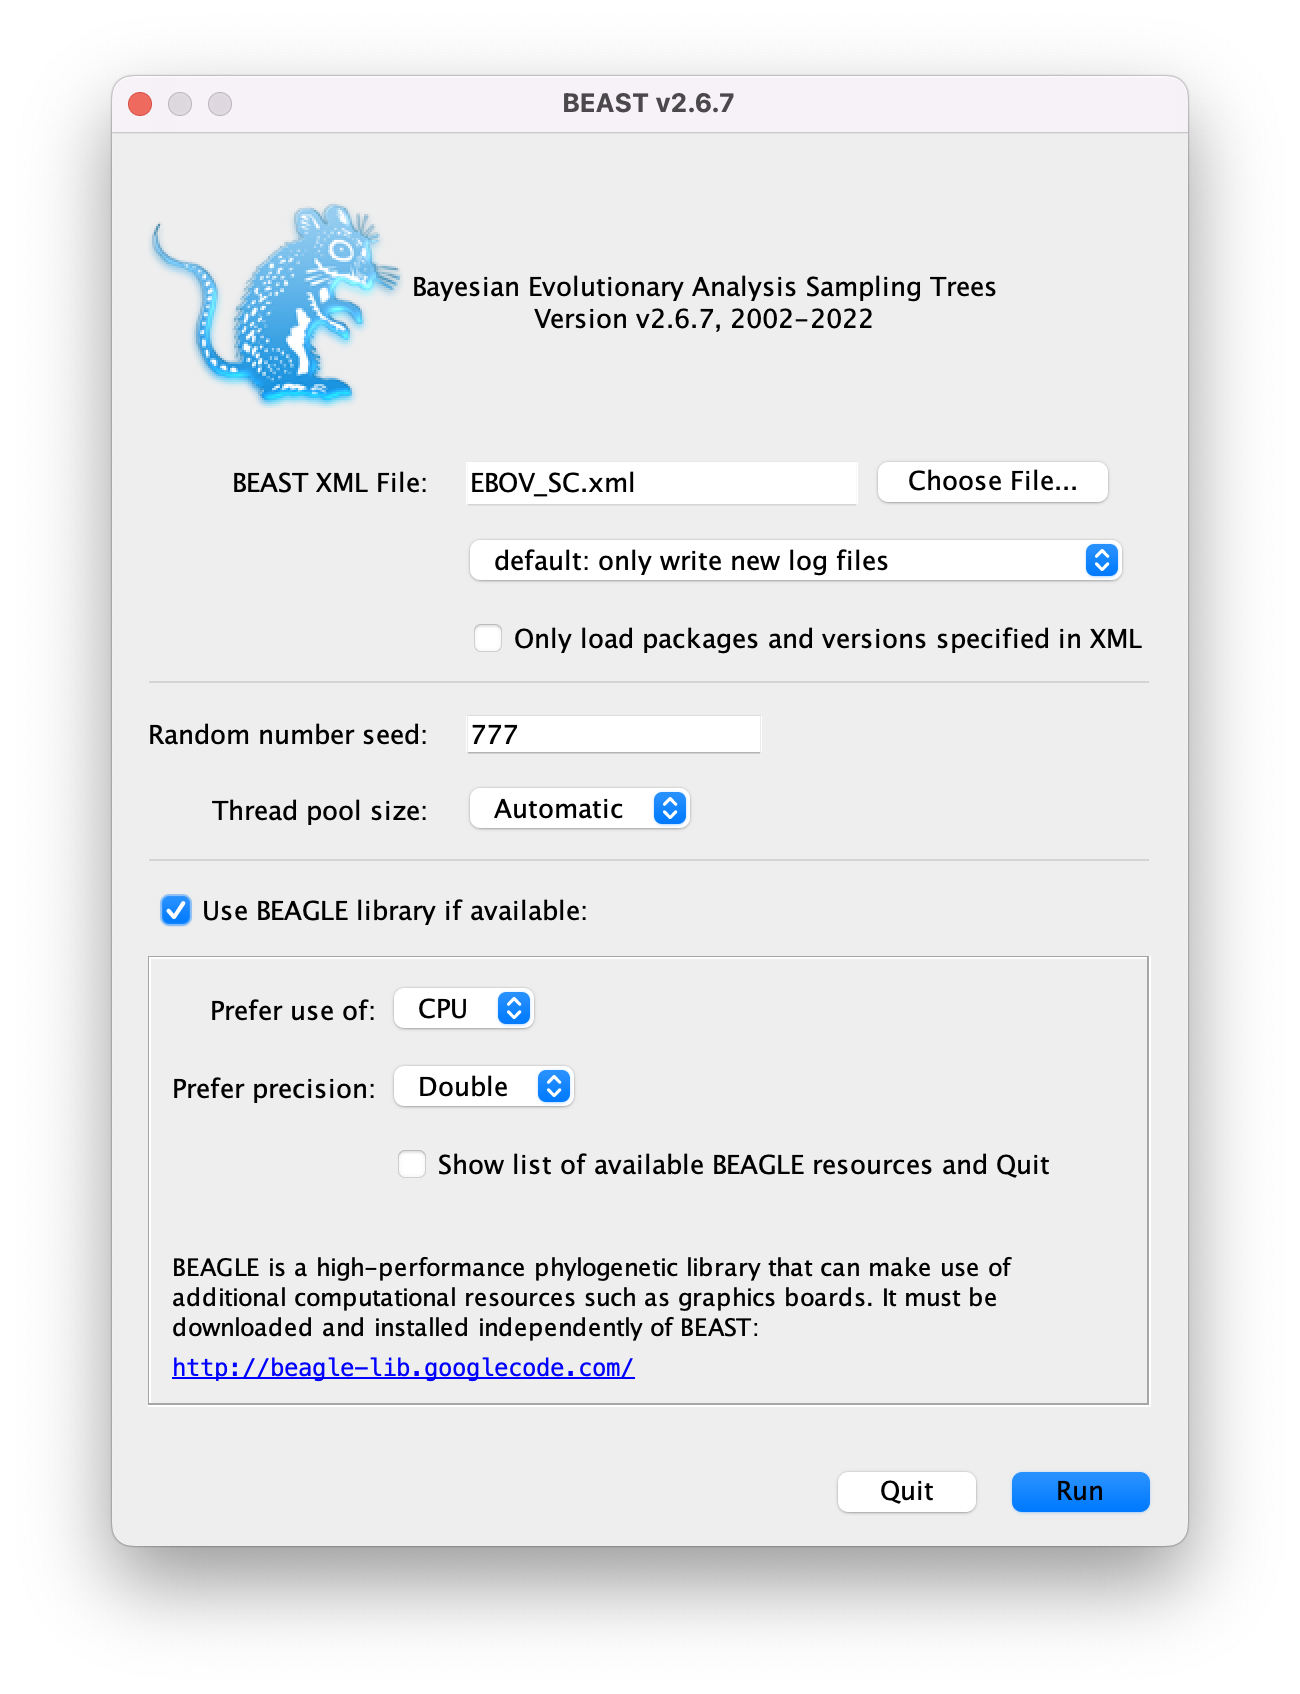
\includegraphics[width=0.800000\textwidth]{figures/beast.png}
    \caption{BEAST2 setup for the analysis.}
    \label{fig:beast}
\end{figure}

The BEAST2 window should look as shown in Figure \ref{fig:beast}.

\begin{framed}
Run \textbf{BEAST2} by clicking the \lstinline!Run! button.
\end{framed}

BEAST2 will run until the specified number of steps in the chain is
reached. While it is running, it will print the screenlog values to a
console and store the tracelog and tree log values to files located in
the same folder as the configuration XML file. The screen output will
look approximately as shown in Figure \ref{fig:beast_out}.

\begin{figure}
    \centering
    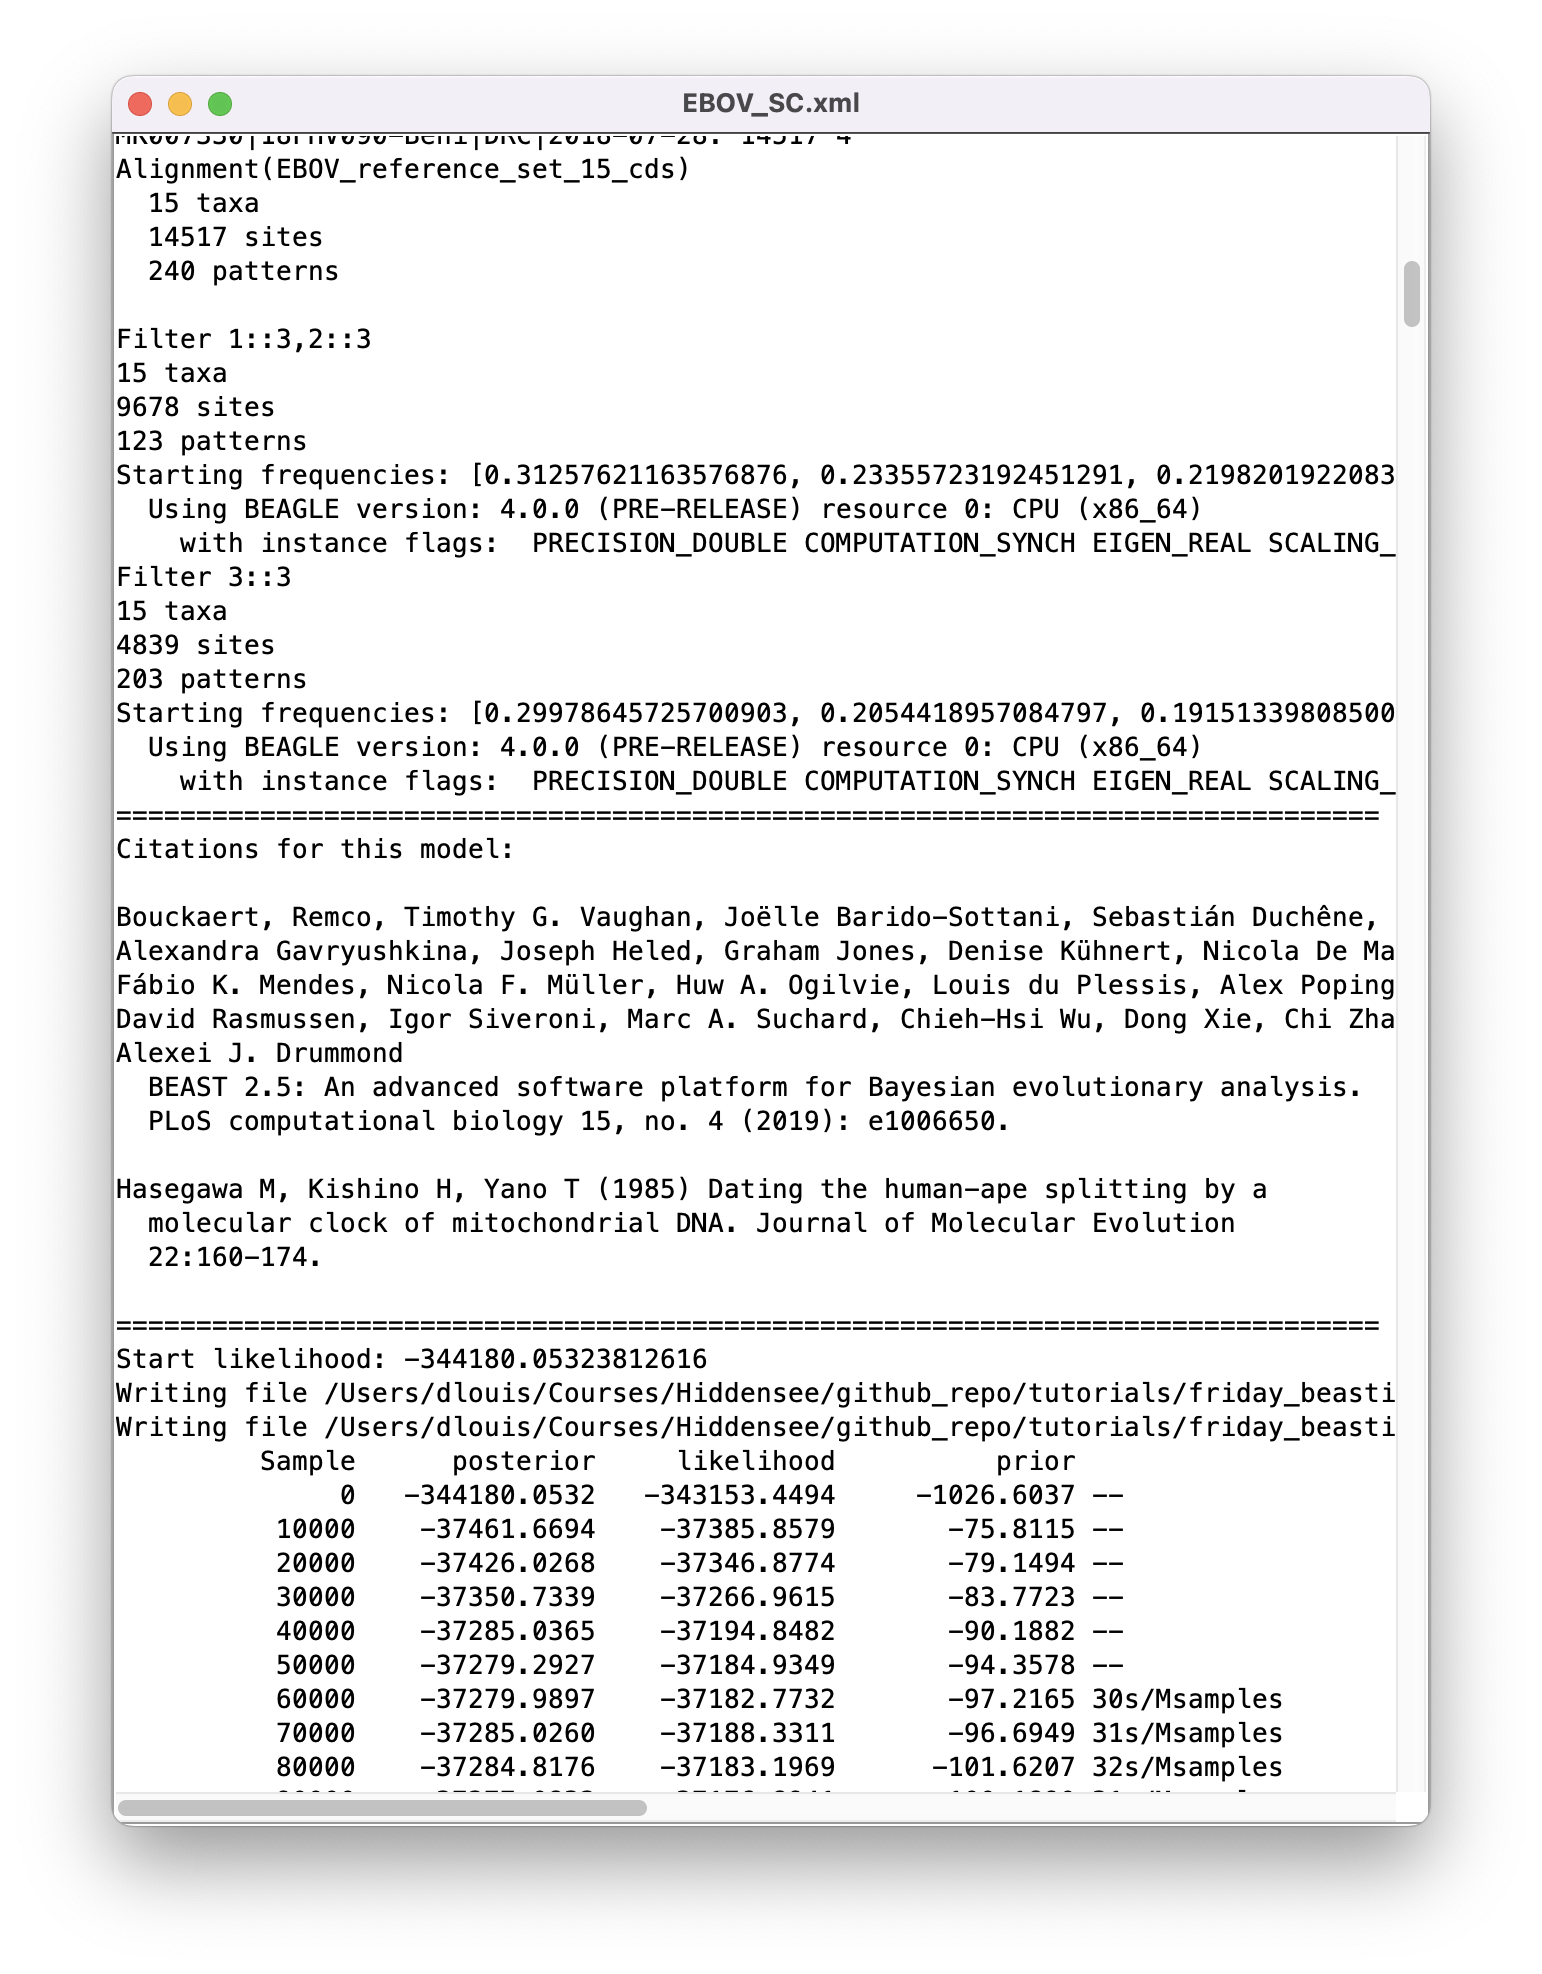
\includegraphics[width=0.800000\textwidth]{figures/beast_out.png}
    \caption{BEAST2 screen output for the analysis.}
    \label{fig:beast_out}
\end{figure}

The window will remain open when BEAST2 finished running the analysis.
When you try to close it, you may see BEAST2 asking the question: ``Do
you wish to save?''. Note that your log and trees files are always
saved, no matter what answer you choose for this question. Thus, the
question is only restricted to saving the BEAST2 screen output (which
contains some information about the hardware configuration, initial
values, operator acceptance rates and running time that are not stored
in the other output files).


\begin{framed}
\textbf{Topic for discussion:} While the analysis is running see if you
can identify which parts of the setup in BEAUti are concerned with the
data, the model and the MCMC algorithm.

Open the XML file in your favourite text editor. Can you recognize any
of the values you set in BEAUti? Can you identify the data, model
specification and MCMC settings in the XML file?

Can you find the likelihood, priors and hyperpriors in the XML file?
\end{framed}

\clearpage


\subsection{Analysing the results}\label{analysing-the-results}

Once BEAST2 has finished running, open Tracer to get an overview of
BEAST2 output. When the main window has opened, choose
\lstinline!File > Import Trace File...! and select the file called
\lstinline!EBOV_SC.log! that BEAST2 has created, or simply drag
the file from the file manager window into Tracer.

\begin{framed}
Open \textbf{Tracer}. Drag and drop the \lstinline!EBOV_SC.log!
file into the open Tracer window.

Alternatively, use \textbf{File \textgreater{} Import Trace
File\ldots{}} (or press the \textbf{+} button below the \textbf{Trace
Files} panel) then locate and click on \lstinline!EBOV_SC.log!.
\end{framed}

The Tracer window should look as shown in Figure \ref{fig:tracer_bad}.

\begin{figure}
    \centering
    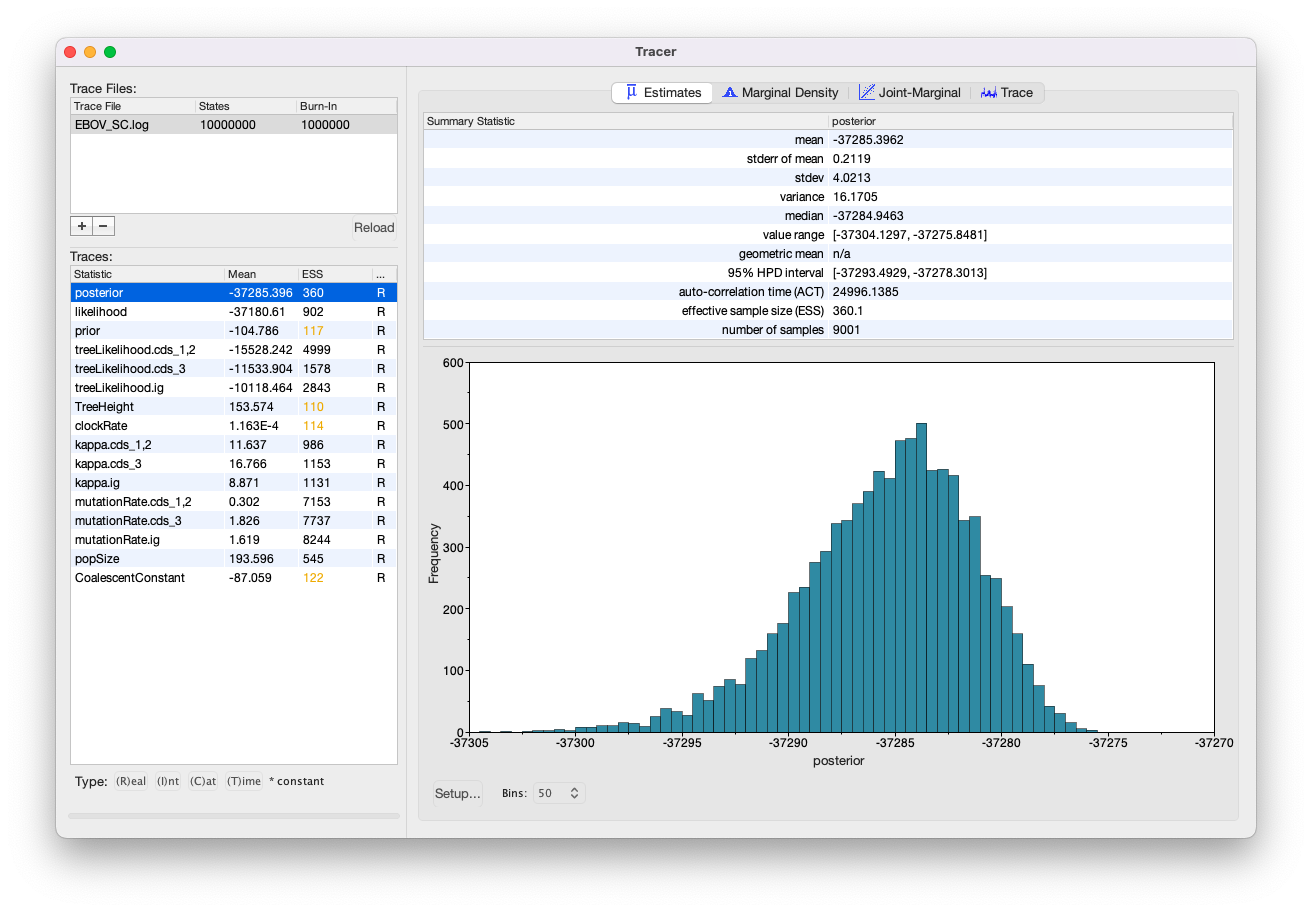
\includegraphics[max width=\textwidth, max height=0.9\textheight]{figures/tracer_bad.png}
    \caption{Tracer showing a summary of the BEAST2 run of the strict clock analysis with an MCMC chain length of 10'000'000 and no constraints.}
    \label{fig:tracer_bad}
\end{figure}

Tracer provides a few useful summary statistics on the results of the
analysis. On the left side in the top window it provides a list of log
files loaded into the program. The window below shows the
list of statistics logged in each file. For each statistic it gives a
list of summary values such as the mean, standard error, median, and
others it can compute from the data. The summary values are displayed in
the top right window and a histogrom showing the distribution of the
statistic is in the bottom right window.

The log file contains traces for the posterior (this is the natural
logarithm of the product of the tree likelihood and the prior density),
prior, the likelihood, tree likelihoods and other continuous parameters.
Selecting a trace on the left brings up the summary statistics for this
trace on the right hand side. When first opened, the \textbf{posterior}
trace is selected and various statistics of this trace are shown under
the \textbf{Estimates} tab.

For each loaded log file we can specify a \textbf{Burn-In}, which is
shown in the file list table (top left) in Tracer. The burn-in is
intended to give the Markov Chain time to reach its equilibrium
distribution, particularly if it has started from a bad starting point.
A bad starting point may lead to over-sampling regions of the posterior
that actually have very low probability under the equilibrium
distribution, before the chain settles into the equilibrium
distribution. Burn-in allows us to simply discard the first \emph{N}
samples of a chain and not use them to compute the summary statistics.
Determining the number of samples to discard is not a trivial problem
and depends on the size of the dataset, the complexity of the model and
the length of the chain. A good rule of thumb is to always throw out at
least the first 10\% of the whole chain length as the burn-in (however,
in some cases it may be necessary to discard as much as 50\% of the MCMC
chain).

Select the \textbf{TreeHeight} statistic in the left hand list to look
at the tree height estimated jointly for all partitions in the
alignment. Tracer plots the (marginal posterior) histogram for the
selected statistic and also gives you summary statistics such as the mean
and median. The 95\% HPD stands for \emph{highest posterior density
interval} and represents the most compact interval on the selected
statistic that contains 95\% of the posterior density. It can be loosely
thought of as a Bayesian analogue to a confidence interval. The
\textbf{TreeHeight} statistic gives the marginal posterior distribution
of the age of the root of the entire tree (that is, the tMRCA; the time to the 
most recent common ancestor).

\begin{framed}
Select \textbf{TreeHeight} in the bottom left hand list in Tracer and
view the different summary statistics on the right.
\end{framed}

You can also compare estimates of different parameters in Tracer. Once a
trace file is loaded into the program you can, for example, compare
estimates of the different mutation rates corresponding to the different
partitions in the alignment.

\begin{framed}
Select all three mutation rates by clicking the first mutation rate
(\textbf{mutationRate.cds\_1,2}), then holding \textbf{Shift} and
clicking the last mutation rate (\textbf{mutationRate.ig}).

Select the \textbf{Marginal Density} tab on the right to view the four
distributions together.

Select different options in the \textbf{Display} drop-down menu to
display the posterior distributions in different ways.
\end{framed}

You will be able to see all four distributions in one plot, similar to
what is shown in Figure \ref{fig:tracer_comparison}.

\begin{figure}
    \centering
    %\includegraphics[max width=\textwidth, max height=0.9\textheight]{figures/Tracer_comparison_KDE.png}
    \includegraphics[max width=0.5\textwidth]{figures/Tracer_KDE.png}
    \includegraphics[max width=0.5\textwidth]{figures/Tracer_violin.png}
    \includegraphics[max width=0.5\textwidth]{figures/Tracer_box.png}
    \caption{Tracer showing the four marginal probability distributions of the mutation rates in each partition of the alignment. The figure at the top shows the marginal distributions plotted with a Kernel Density Estimation (KDE) in the middle as violin plots and at the bottom as box and whisker plots. Note that you 
    can also display a legend.}
    \label{fig:tracer_comparison}
\end{figure}

\begin{framed}
\textbf{Topic for discussion:} What can you deduce from the marginal
densities of the 4 mutation rates? Does this make biological sense?
\end{framed}






\subsubsection{Analysing tree estimates}\label{analysing-tree-estimates}

Besides producing a sample of parameter estimates, BEAST2 also produces
a posterior sample of time-calibrated phylogenetic trees. These need to be
summarised too before any conclusions about the quality of the posterior
estimate can be made.

One way to summarise the trees is by using the program TreeAnnotator.
This will take the set of trees and find the \emph{maximum clade credibility} 
tree, which is one particular estimate of the ``best supported'' tree.
The nodes in this tree are also annotated with the corresponding 95\% HPD 
ranges in the posterior set of trees and each clade is annotated with 
its posterior probability.

\begin{framed}
Open \textbf{TreeAnnotator}.

Set the \textbf{Burnin percentage} to \textbf{10\%} to discard the first
10\% of trees in the tree file.
\end{framed}

The next option, the \textbf{Posterior probability limit}, specifies a
limit such that if a node is found at less than this frequency in the
sample of trees (i.e.~has a posterior probability less than this limit),
it will not be annotated. For example, setting it to 0.5 means that only
nodes seen in the majority (more than 50\%) of trees will be annotated.
The default value is 0, which we will leave as is, and which means that
TreeAnnotator will annotate all nodes.

\begin{framed}
Leave the \textbf{Posterior probability limit} at the default value of
\textbf{0}.
\end{framed}

For the \textbf{Target tree type} option you can either choose a
specific tree from a file or ask TreeAnnotator to find a tree in your
sample. The default option which we will leave, \textbf{Maximum clade
credibility tree}, finds the tree with the highest product of the
posterior probability of all its nodes.

\begin{framed}
Leave the \textbf{Target tree type} at the default value of
\textbf{Maximum clade credibility tree}.
\end{framed}

Next, select \textbf{Mean heights} for the \textbf{Node heights}. This
sets the heights (ages) of each node in the tree to the mean height
across the entire sample of trees for that clade.

\begin{framed}
Select \textbf{Mean heights} in the \textbf{Node heights} drop-down
menu.
\end{framed}

Finally, we have to select the input tree log file and set an output
file.

\begin{framed}
Click \textbf{Choose File} next to \textbf{Input Tree File} and choose
\lstinline!EBOV_SC.trees!.

Set the \textbf{Output File} to \lstinline!EBOV_SC.MCC.tree!.
\end{framed}

The setup should look as shown in Figure \ref{fig:treeannot}. You can
now run the program.

\begin{figure}
    \centering
    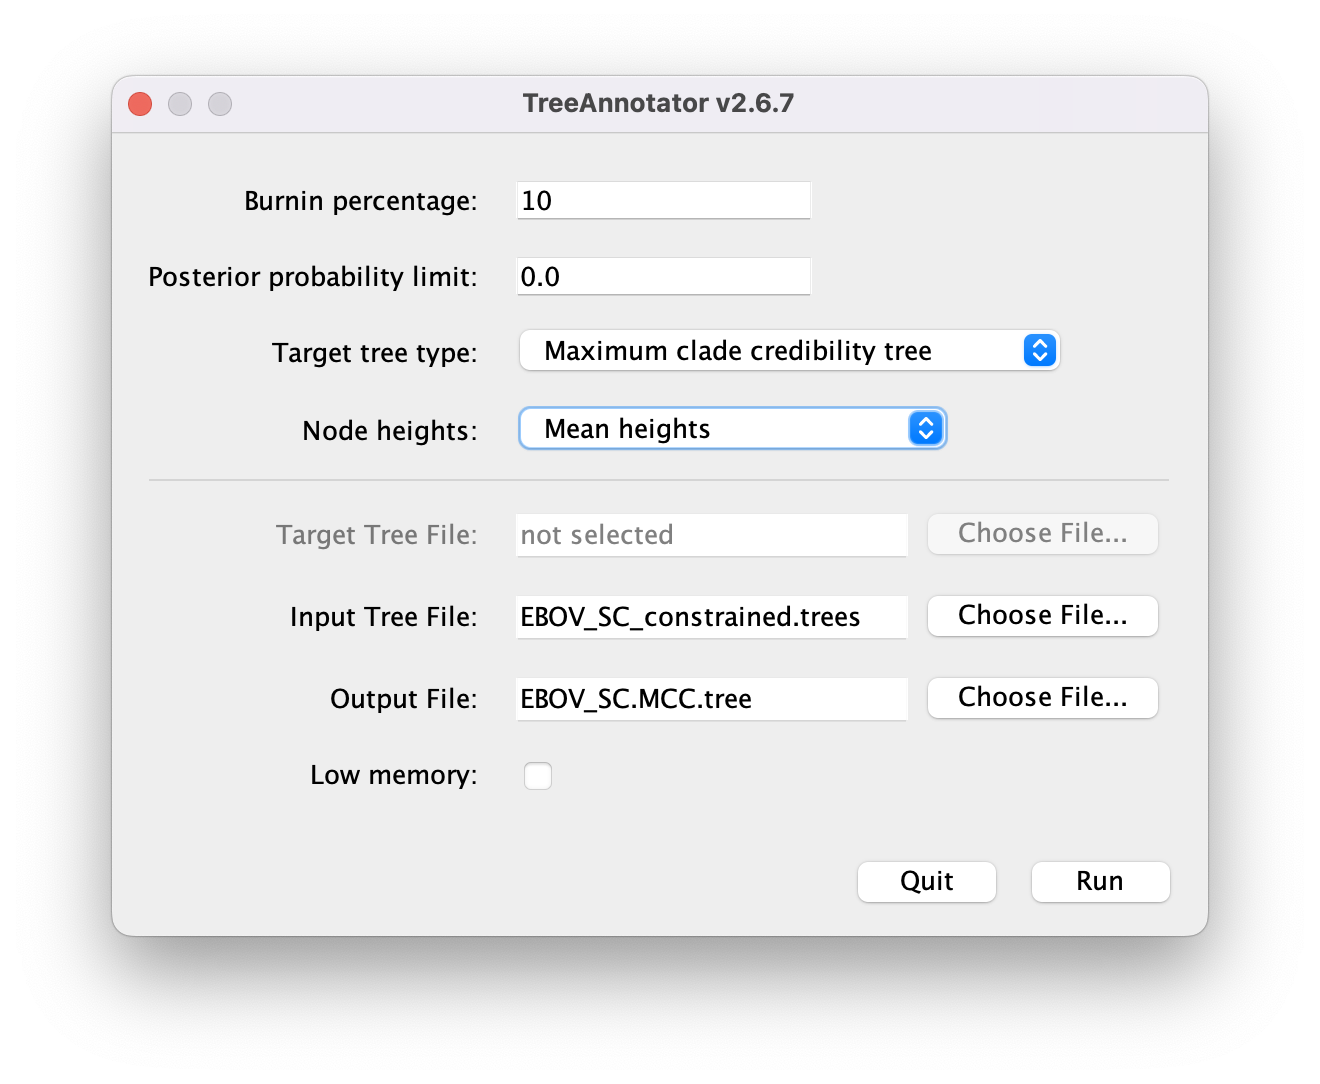
\includegraphics[width=0.800000\textwidth]{figures/treeannot.png}
    \caption{TreeAnnotator setup}
    \label{fig:treeannot}
\end{figure}

\subsubsection{Visualising the tree
estimate}\label{visualising-the-tree-estimate}

Finally, we can visualize the tree with one of the available pieces of
software, such as FigTree.

\begin{framed}
Open \textbf{FigTree}. Use \textbf{File \textgreater{} Open} then locate
and click on \lstinline!EBOV_SC.MCC.tree!.

\begin{itemize}

\item
  Expand \textbf{Trees} options, check \textbf{Order nodes} and select
  \textbf{decreasing} from the drop-down menu.
\item
  Expand the \textbf{Tip Labels} options and increase the \textbf{Font
  Size} until it is readable.
\item
  Check the \textbf{Node Bars} checkbox, expand the options and select
  \lstinline!height_95%_HPD! from the \textbf{Display} drop-down menu.
\item
  Check the \textbf{Node Labels} checkbox, expand the options and select
  \lstinline!posterior! from the \textbf{Display} drop-down menu.
\item
  Increase the \textbf{Font Size} until it is readable.
\item
  Uncheck the \textbf{Scale Bar} checkbox.
\item
  Check the \textbf{Scale Axis} checkbox, expand the options, check
  \textbf{Reverse axis} and increase the \textbf{Font Size}.
\item
  Expand the \textbf{Time Scale} options and set the offset to 2018 
  (approximately the most recent collection date). 
\end{itemize}
\end{framed}

\begin{figure}
    \centering
    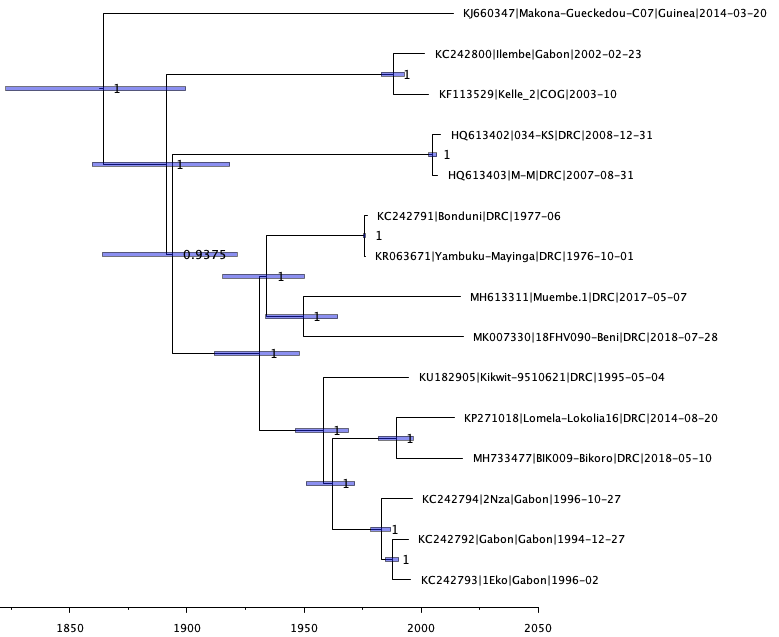
\includegraphics[max width=0.8\textwidth, max height=0.9\textheight]{figures/figtree_SC.png}
    \caption{FigTree visualisation of the estimated tree.}
    \label{fig:figtree}
\end{figure}

Your tree should now look something like Figure \ref{fig:figtree}. We
first ordered the tree nodes. Because there are many ways to draw the
same tree, ordering nodes makes it easier for us to compare different
trees to each other. The scale bars we added represent the 95\% HPD
interval for the age of each node in the tree, as estimated by the
BEAST2 analysis. The node labels we added gives the posterior
probability for a node in the posterior set of trees (that is, the trees
logged in the tree log file, after discarding the burn-in). We can also
use FigTree to display other statistics, such as the branch lengths, the
95\% HPD interval of a node etc. The exact statistics available will
depend on the model used.

We can see that the tree topology is very highly supported, although there 
is some uncertainty in the age of the deeper nodes. We also see that 
the representative genome of the 2014 West African Ebola virus disease
epidemic (Makona-Gueckedou-C07) is an outgroup to all other genomes in our 
dataset and that the tMRCA is estimated to be around the middle of the 19th 
century. 


\subsection{Adding topology constraints}
\citet{Dudas2014} found in a different analysis that the root
most likely lies between the outbreaks of the 1970s and the other outbreaks. In other words, 
they found that the MRCA (most recent common ancestor) of all known human EBOV outbreaks was 
closest to the viruses that caused the 1970s outbreaks. 
Armed with this prior knowledge, how can we incorporate it in our analysis? 
We can set a monophyly constraint to 
tell BEAST2 that a certain group of sequences should form a single clade in the tree
with a common ancestor! Implicitly that will also constrain the MRCA of this clade
to be younger than the tree's root. We can do this in BEAUti. 

Either set up a new XML file in BEAUti and follow the same steps as above
until you've specified the priors or else simply go back to BEAUti and edit the previous 
analysis file. 

\begin{framed}
To add an extra prior to the model, Click on the \textbf{Priors} tab and click
the \textbf{+ Add Prior} button below the list of priors and select \textbf{MRCA Prior} 
from the drop-down menu.

You will see a dialogue box that allows you to select a subset of taxa
from the phylogenetic tree. 

\begin{itemize}

\item
  Set the \textbf{Taxon set label} to \lstinline!ingroup!.
\item
  Select all sequences on the left hand side list and click
  the \textbf{\textgreater{}\textgreater{}} button to add them to the
  \lstinline!ingroup! taxon set.
\item
  Locate \lstinline!Bonduni! and \lstinline!Yambuku-Mayinga! sequences on 
  the right hand side and click \textbf{\textless{}\textless{}} to move them 
  out of the taxon set.
\end{itemize}
\end{framed}

The taxon set should now look like Figure \ref{fig:taxa}.

\begin{framed}
Click the \textbf{OK} button to add the newly defined taxon set to the
prior list.
\end{framed}

\begin{figure}
    \centering
    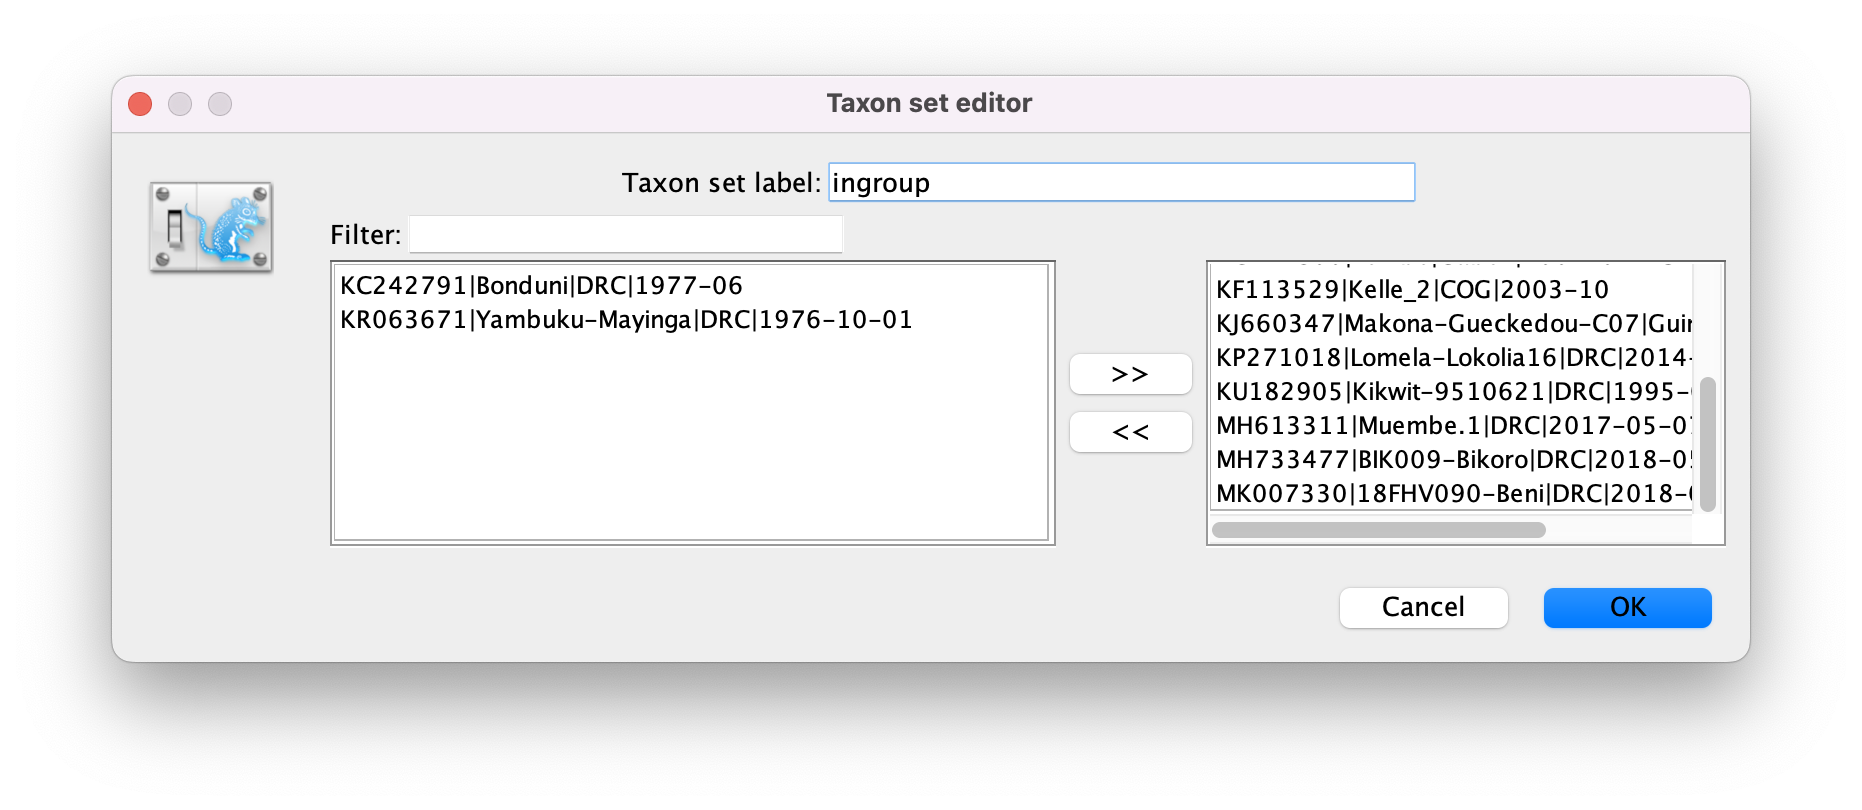
\includegraphics[width=0.800000\textwidth]{figures/taxa.png}
    \caption{Ingroup taxon set.}
    \label{fig:taxa}
\end{figure}

In order to constrain the tree topology to keep our ingroup monophyletic
during the course of the MCMC analysis we have to select monophyletic.

\begin{framed}
Check the \textbf{monophyletic} checkbox next to
\textbf{ingroup.prior}.
\end{framed}

We could now also add calibration information for its most recent common
ancestor (MRCA). We can do this by adding a prior on the age of the MRCA 
node of our taxon set. However, we can only do this if we have some 
prior information about its age, which we do not have here so any such prior would 
be pure guesswork.

Leave the MCMC settings as before, but change the filenames to \lstinline!EBOV_SC_constrained.log! and 
\lstinline!EBOV_SC_constrained.trees!. Now save the XML file as \lstinline!EBOV_SC_constrained.xml! and run it
in BEAST2 (with seed 777).



\subsection{Setting up a relaxed clock analysis}
While the constrained strict clock analysis is running we will set up a similar analysis, 
but using a relaxed clock this time. 
Whereas the strict clock enforced the same molecular clock rate on all 
branches in the tree, a relaxed clock allows for rate variation among 
branches. 

We have a good intuition that there should be rate variation. When the first genomes 
from the 2014 Ebola virus disease outbreak in the Democratic Republic of the Congo were 
sequenced, it was noted that they were much less divergent from earlier EBOV genomes than those
sequenced from the 2014 West African Ebola virus disease epidemic \citep{Maganga2014}. 
Long-term periods of latency had also been observed during the West African epidemic 
\citep{Blackley2016, Diallo2016}. These observations suggested that latency or possibly different 
animal reservoirs \citep{Lam2015} could be responsible for the observed discrepancies in 
genetic distances that were observed for the 2014 genomes. The same lower divergence was also 
observed for genomes from teh 2017 and 2018 outbreaks in the Democratic Republic of the Congo 
(\url{http://beast.community/ebov_local_clocks.html}).


\begin{framed}
Click on the \textbf{Clock Models} tab and select \lstinline!Relaxed Clock Log Normal!
from the dropdown box.
\end{framed}

This will use an uncorrelated lognormally distributed relaxed clock model. This model 
allows each branch in the tree to have a different rate, independently drawn from a lognormal
distribution \citep{Drummond2006}. This is a very flexible model and is the most popular relaxed clock model 
for viral genomes. However, it should not be used as a default model for every analysis!

The relaxed clock has two parameters, for which we need to set priors. These parameters describe
the mean and the standard deviation of the lognormal distribution from which the clock rates of 
the tree branches are drawn. 

\begin{framed}
  Click on the \textbf{Priors} tab. 

  For \textbf{ucldMean.c:clock} we will use the same exponential prior we used for the 
  clock rate in the strict clock analysis. We will leave the prior for \textbf{ucldStdev}
  as the default.
\end{framed}

Leave the MCMC settings as before, but change the filenames to \lstinline!EBOV_UCLD_constrained.log! and 
\lstinline!EBOV_UCLD_constrained.trees!. Now save the XML file as \lstinline!EBOV_UCLD_constrained.xml! and run it
in BEAST2 (with seed 777).







\subsection{Comparing results and checking convergence}\label{comparing-results-and-checking-convergence}

Two very important summary statistics that we should pay attention to
are the Auto-Correlation Time (ACT) and the Effective Sample Size (ESS).
ACT is the average number of states in the MCMC chain that two samples
have to be separated by for them to be uncorrelated, i.e.~for them to be
independent samples from the posterior. The ACT is estimated from the
samples in the trace (excluding the burn-in). The ESS is the number of
independent samples that the trace is equivalent to. This is calculated
as the chain length (excluding the burn-in) divided by the ACT.

The ESS is regarded as a good quality-measure of the resulting
sample sequence. It is unclear how to determine exactly how large should
the ESS be for the analysis to be trustworthy. In general, an ESS of 200
is considered high enough to make the analysis useful. However, this is
an arbitrary number and you should always use your own judgment to
decide if the analysis has converged or not. ESS values below 100 are coloured in red, 
which means that we should (probably) not trust the value of the statistics, and ESS
values between 100 and 200 are coloured in yellow.

If a lot of statistics have red or yellow coloured ESS value, we have
not sufficiently explored the posterior space. This is most likely a
result of the chain not running long enough. 

\begin{framed}
  Load the log files of all three XML files into Tracer. 

  Click on the \textbf{Trace} tab to look at the traces of parameters.
\end{framed}

You'll notice that both of the constrained analyses have several parameters
with very low ESS values below 100 (Figure~\ref{fig:tracer_terrible}). Looking
at the traces of these parameters it is clear that they are having some trouble
mixing and that we definitely need to run our analyses longer. Luckily it doesn't 
look like any of these parameters  have ``sticky'' chains!

\begin{figure}
    \centering
    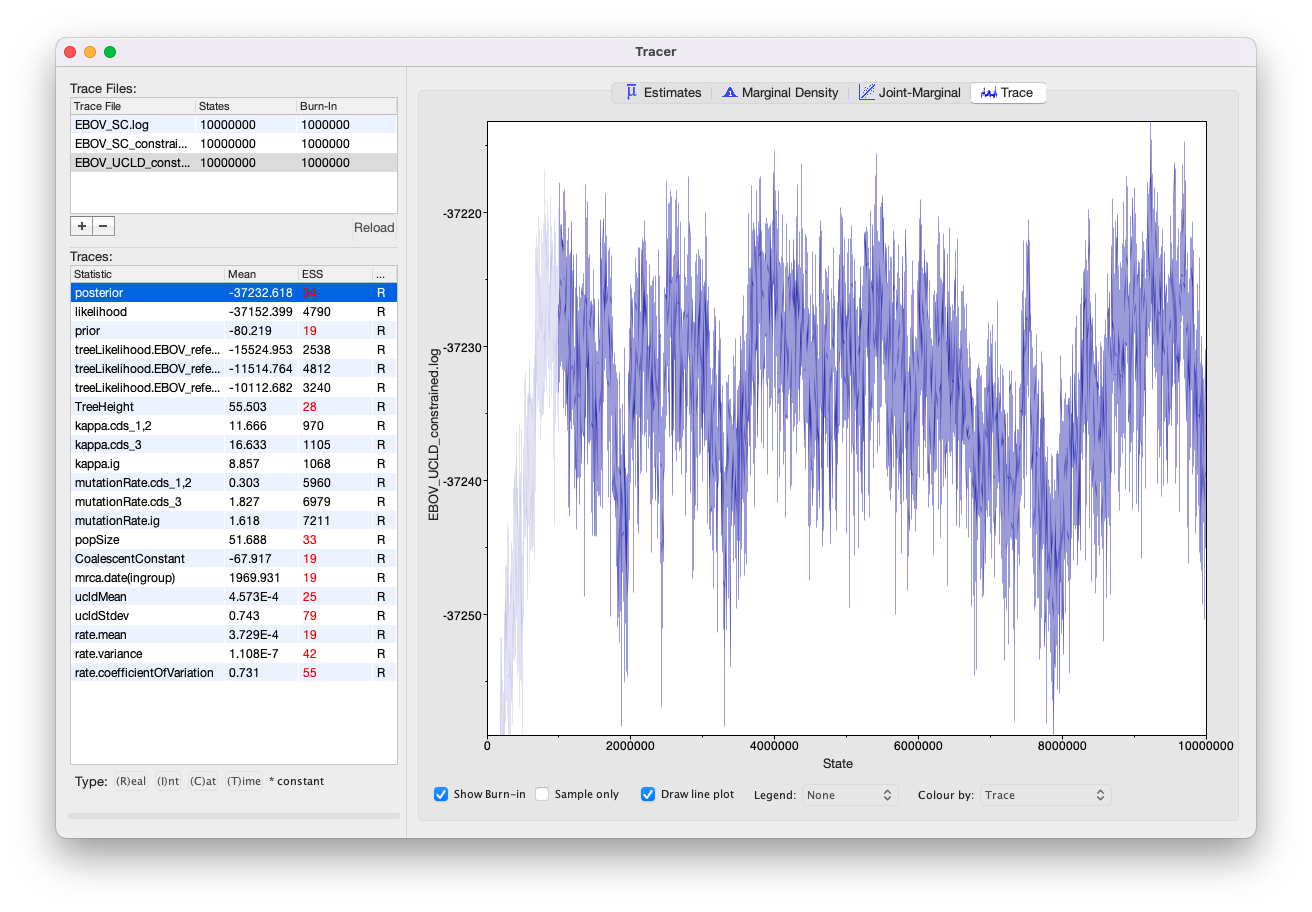
\includegraphics[max width=\textwidth, max height=0.9\textheight]{figures/tracer_terrible.png}
    \caption{Trace with a poor ESS value.}
    \label{fig:tracer_terrible}
\end{figure}

\begin{framed}
  Select all three log files in the left-hand panel to show all shared parameters
  between them. 
\end{framed}

We note that both of the constrained analyses resulted in much younger estimates for 
the tMRCA (Figure~\ref{fig:tracer_ages}. We also note that these two analyses also logged the age of the tMRCA of 
the ingroup, with the relaxed clock analysis estimating the youngest age (Figure~\ref{fig:tracer_tmrca}).

\begin{figure}
    \centering
    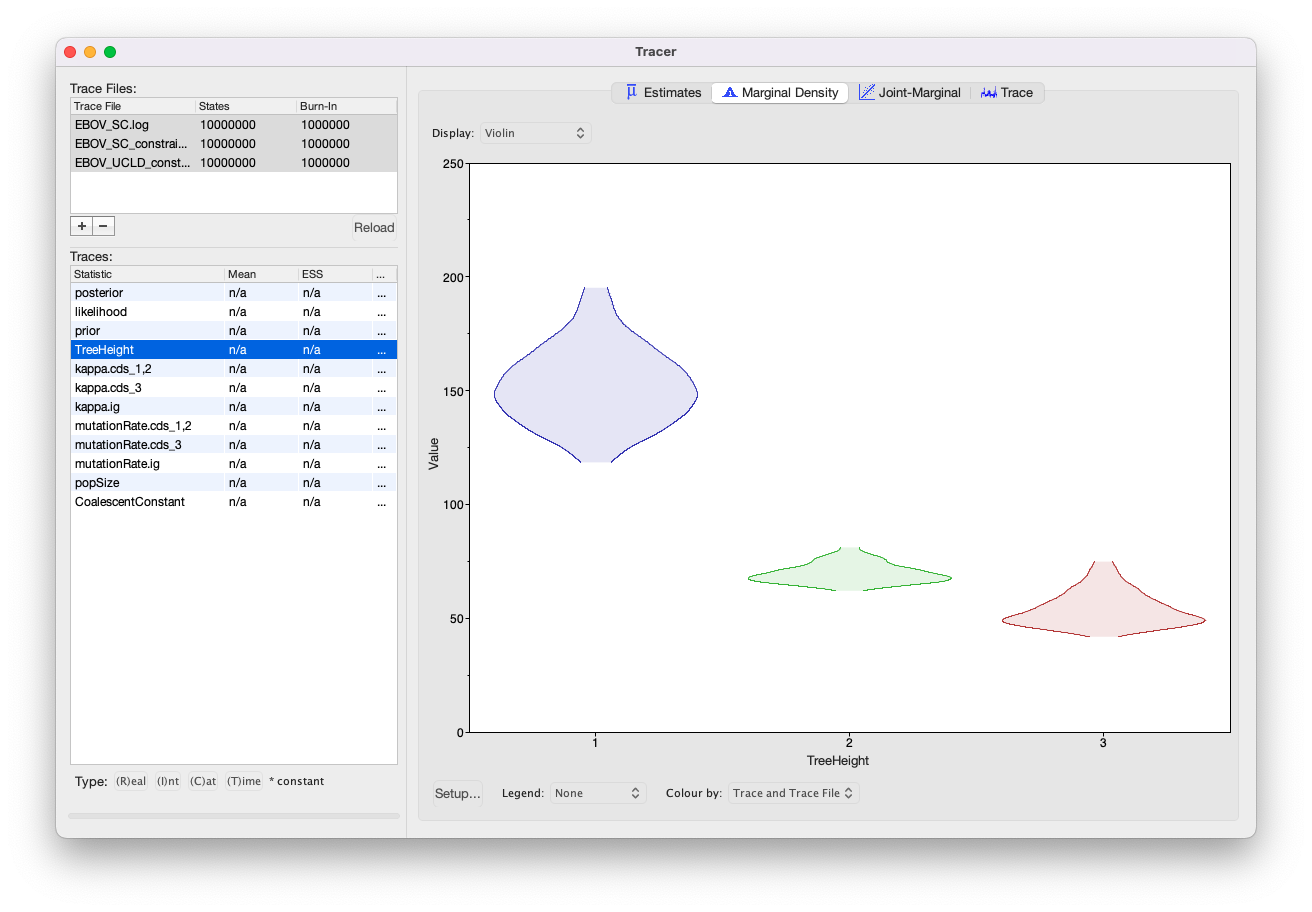
\includegraphics[max width=\textwidth, max height=0.9\textheight]{figures/tracer_ages.png}
    \caption{The posterior height estimates of the three trees.}
    \label{fig:tracer_ages}
\end{figure}
  
\begin{figure}
    \centering
    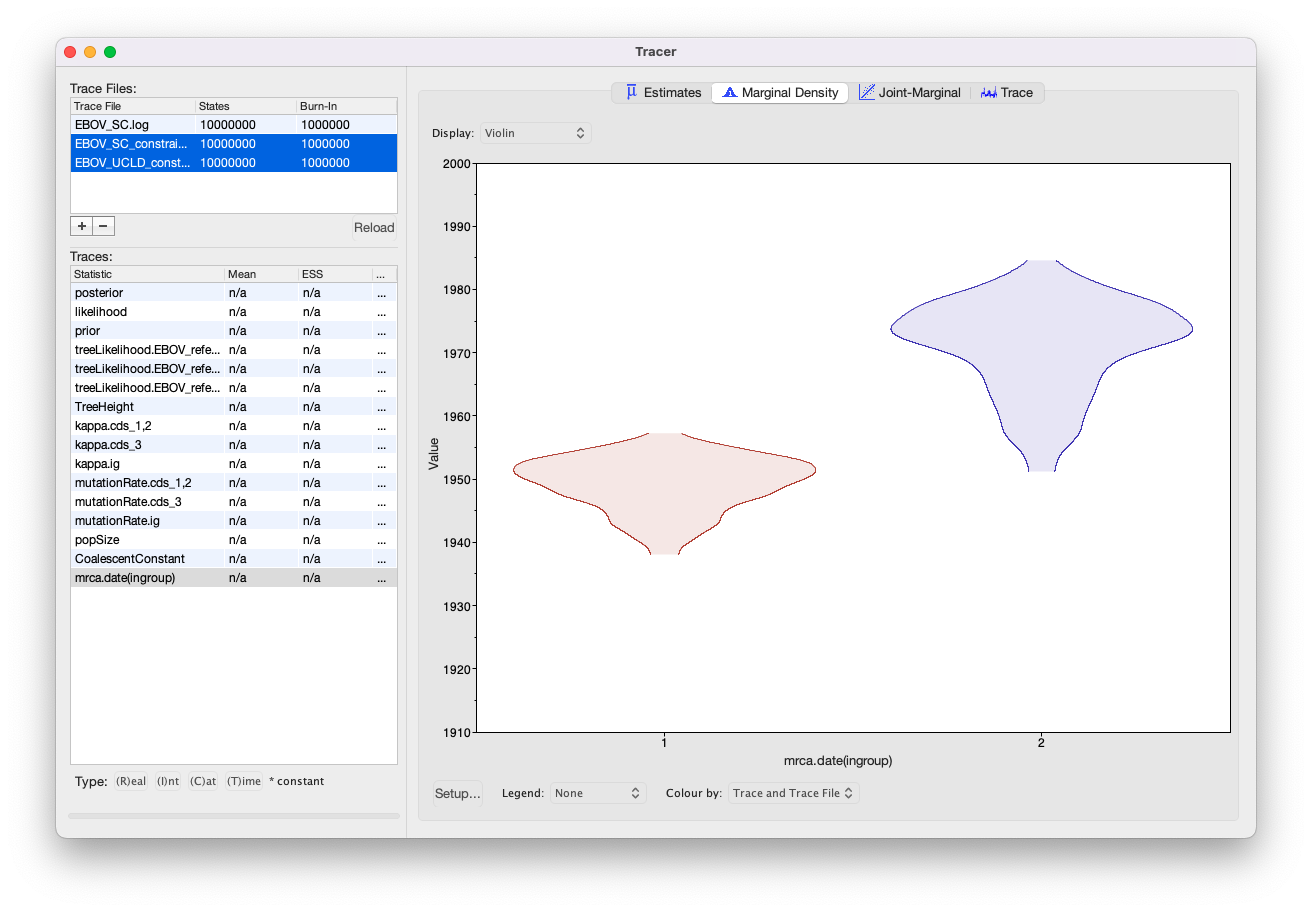
\includegraphics[max width=\textwidth, max height=0.9\textheight]{figures/tracer_tmrca.png}
    \caption{The posterior tMRCAs of the ingroup.}
    \label{fig:tracer_tmrca}
\end{figure}

We also note that the coefficient of variation of the clock rate of the relaxed clock model has an 
HPD interval that does not include 0 (Figure~\ref{fig:coeffvar}). If the coefficient of variation is
0 all rates are equal and the relaxed clock model reduces to a strict clock model. Thus, we can conclude
that there is posterior evidence for variable rates among branches in the tree.  

\begin{figure}
    \centering
    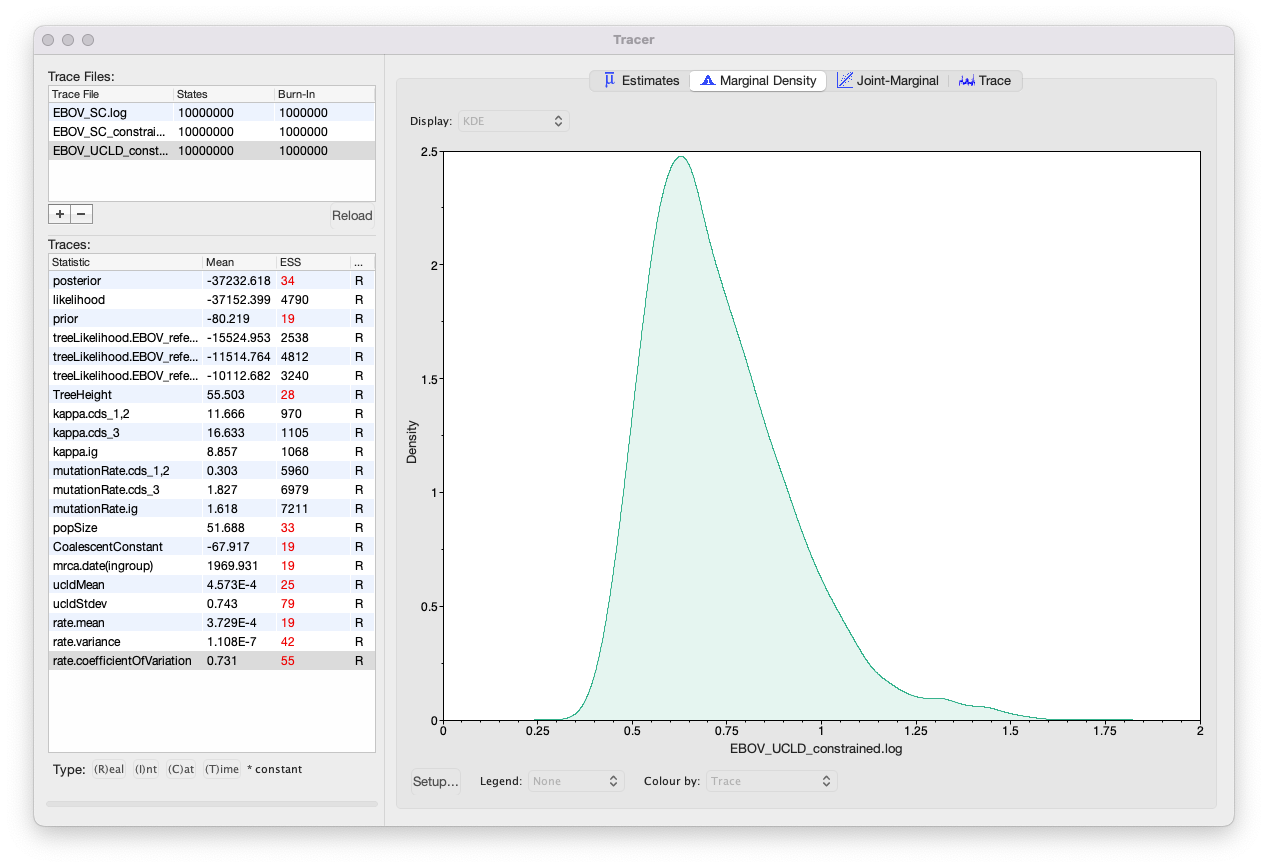
\includegraphics[max width=\textwidth, max height=0.9\textheight]{figures/coeffvar.png}
    \caption{The coefficient of variation of the clock rate of the relaxed clock model.}
    \label{fig:coeffvar}
\end{figure}



Tracer also allows us to look for correlations between parameters under
the \textbf{Joint Marginal} tab, as shown in Figure
\ref{fig:tracer_joint}. When two parameters are highly correlated this
can lead to poor convergence of the MCMC chain.

\begin{figure}
    \centering
    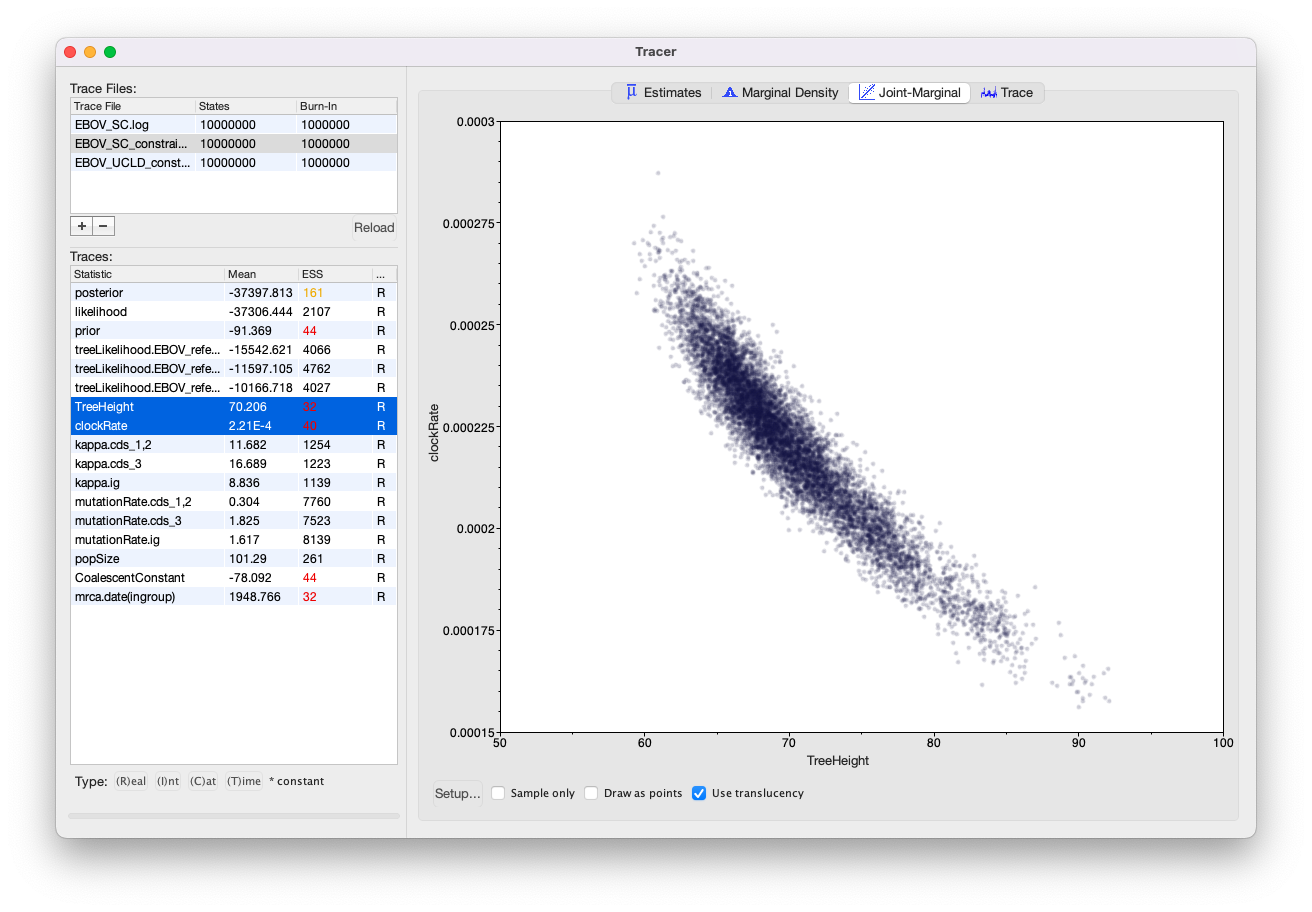
\includegraphics[max width=\textwidth, max height=0.9\textheight]{figures/tracer_joint.png}
    \caption{Correlation between the tree height and clock rate estimates.}
    \label{fig:tracer_joint}
\end{figure}

We can also look at correlations between more than two parameters.

\begin{framed}
Select all 3 mutation rates again

\begin{itemize}

\item
  Navigate to the \textbf{Joint Marginal} tab
\item
  Check \textbf{Show points}
\end{itemize}
\end{framed}

The panel should look like Figure \ref{fig:tracer_covariance}. The ellipses
represent the covariance between pairs of parameters and make it easy to
identify which pairs are correlated or anti-correlated. Is there a
strong correlation or anti-correlation between some of our mutation rate
parameters?

\begin{figure}
    \centering
    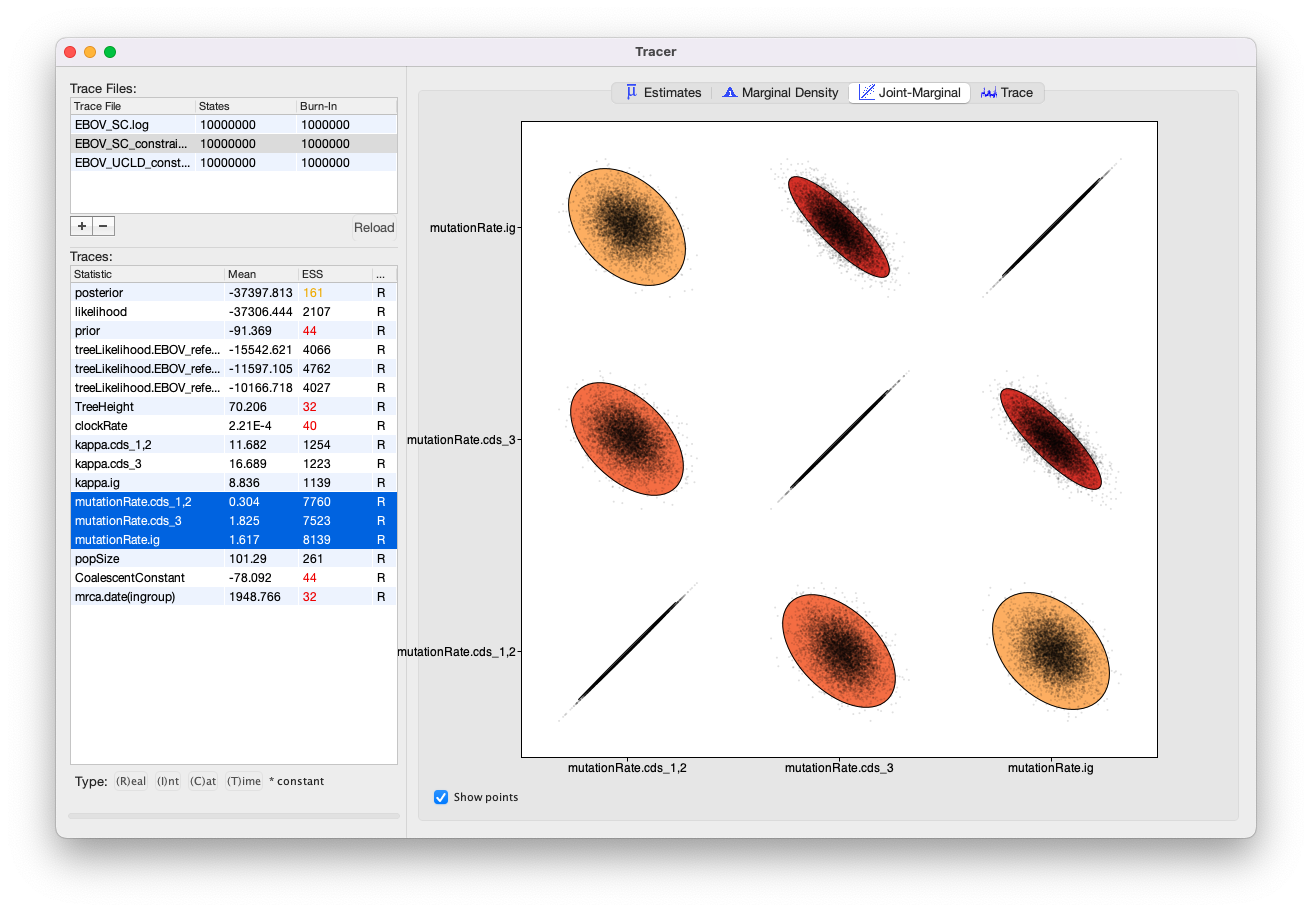
\includegraphics[max width=\textwidth, max height=0.9\textheight]{figures/tracer_covariance.png}
    \caption{Correlations between the mutation rate parameters.}
    \label{fig:tracer_covariance}
\end{figure}



\subsubsection{Visualising rates on trees}\label{visualing-rates-on-trees}

We can usue FigTree to investigate which branches on the tree are inferred to have 
elevated substitution rates under the relaxed clock analysis. 

\begin{framed}
  Open \textbf{TreeAnnotator}.

  Use the same settings as before to create the MCC tree for the relaxed clock analysis and 
  save it as \lstinline!EBOV_UCLD_constrained.MCC.tree!.

  Now open the MCC tree in Figtree.

  \begin{itemize}

  \item
    Expand \textbf{Trees} options, check \textbf{Order nodes} and select
    \textbf{decreasing} from the drop-down menu.
  \item
    Expand the \textbf{Appearance} options and increase the \textbf{Line Weight} to 
    \textbf{4}. Now open the \textbf{Colour by} drop-down menu and select \lstinline!rate_median!
    Finally, click the \textbf{Colours} button and reverse the Hue spectrum (so faster rates are
    hotter and slower rates cooler colours). 
  \item
    Expand the \textbf{Tip Labels} options and increase the \textbf{Font
    Size} until it is readable.
  \item
    Check the \textbf{Branch Labels} checkbox, expand the options and select
    \lstinline!rate_median! from the \textbf{Display} drop-down menu.
  \item
    Increase the \textbf{Font Size} until it is readable.
  \item
    Uncheck the \textbf{Scale Bar} checkbox.
  \item
    Check the \textbf{Scale Axis} checkbox, expand the options, check
    \textbf{Reverse axis} and increase the \textbf{Font Size}.
  \item
    Expand the \textbf{Time Scale} options and set the offset to 2018 
    (approximately the most recent collection date). 
  \item
    Check the \textbf{Legend} checkbox, expand the options and select 
    \lstinline!rate_median! from the \textbf{Attribute} drop-down menu
  \end{itemize}
\end{framed}


\begin{figure}
    \centering
    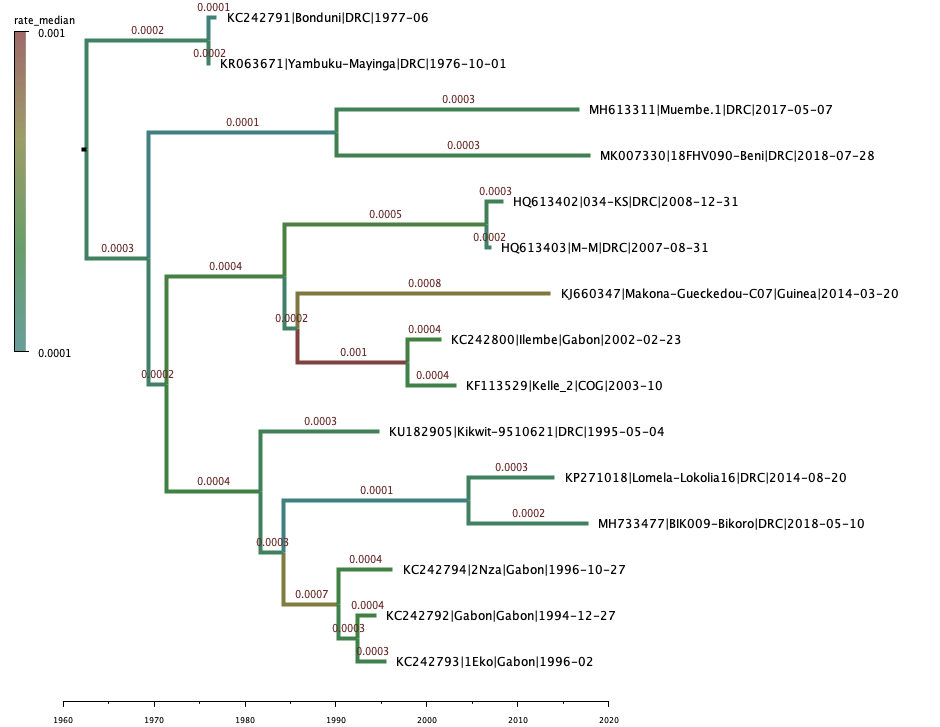
\includegraphics[max width=0.8\textwidth, max height=0.9\textheight]{figures/figtree_UCLD.png}
    \caption{FigTree visualisation of the tree estimated under the relaxed clock model.}
    \label{fig:figtree_ucld}
\end{figure}


The tree should now look something like Figure~\ref{fig:figtree_ucld}. Note that the stem branches 
leading to the 2014, 2017 and 2018 outbreaks in the DRC (Muembe.1, 18FHV090-Beni, Lomela-Lokolia16 and BIK009-Bikoro have 
low median clock rates of $1 \times 10^{-4}$ s/s/y, while the branch leading to the 2014 West African Ebola virus disease
epidemic has a much faster median rate of $8 \times 10^{-4}$ s/s/y. 


\subsection{Setting up a Gamma site model}

Finally, we will return to the discrete Gamma model for modeling site-to-site rate heterogeneity.
We will edit the relaxed clock analysis to also incorporate rate heterogeneity within each of the 
three partitions. In addition, we will also estimate the nucleotide frequencies. 

\begin{framed}
  Select the \textbf{Site Model} tab.

  Make sure that \lstinline!EBOV_reference_set_15_ig! is selected.

  \begin{itemize}
    \item Set the \textbf{Gamma Category Count} to 4.
    \item Check the \textbf{estimate} box for the \textbf{Shape} parameter (it
  should already be checked).
    \item Select \textbf{Estimated} from the \textbf{Frequencies} drop-down
    menu. 
    \item Double-check that the \textbf{estimate} checkbox is ticked for the \textbf{Substitution Rate} and that the 
           \textbf{Subst Model} is set to \textbf{HKY}
  \end{itemize}

  Now use the shortcut to clone the substitution model to all partitions and double-check that each partition now 
  has an HKY model, with 4 Gamma categories, with the shape parameter, frequencies, Kappa and substitution rates 
  estimated.

\end{framed}

\begin{figure}
    \centering
    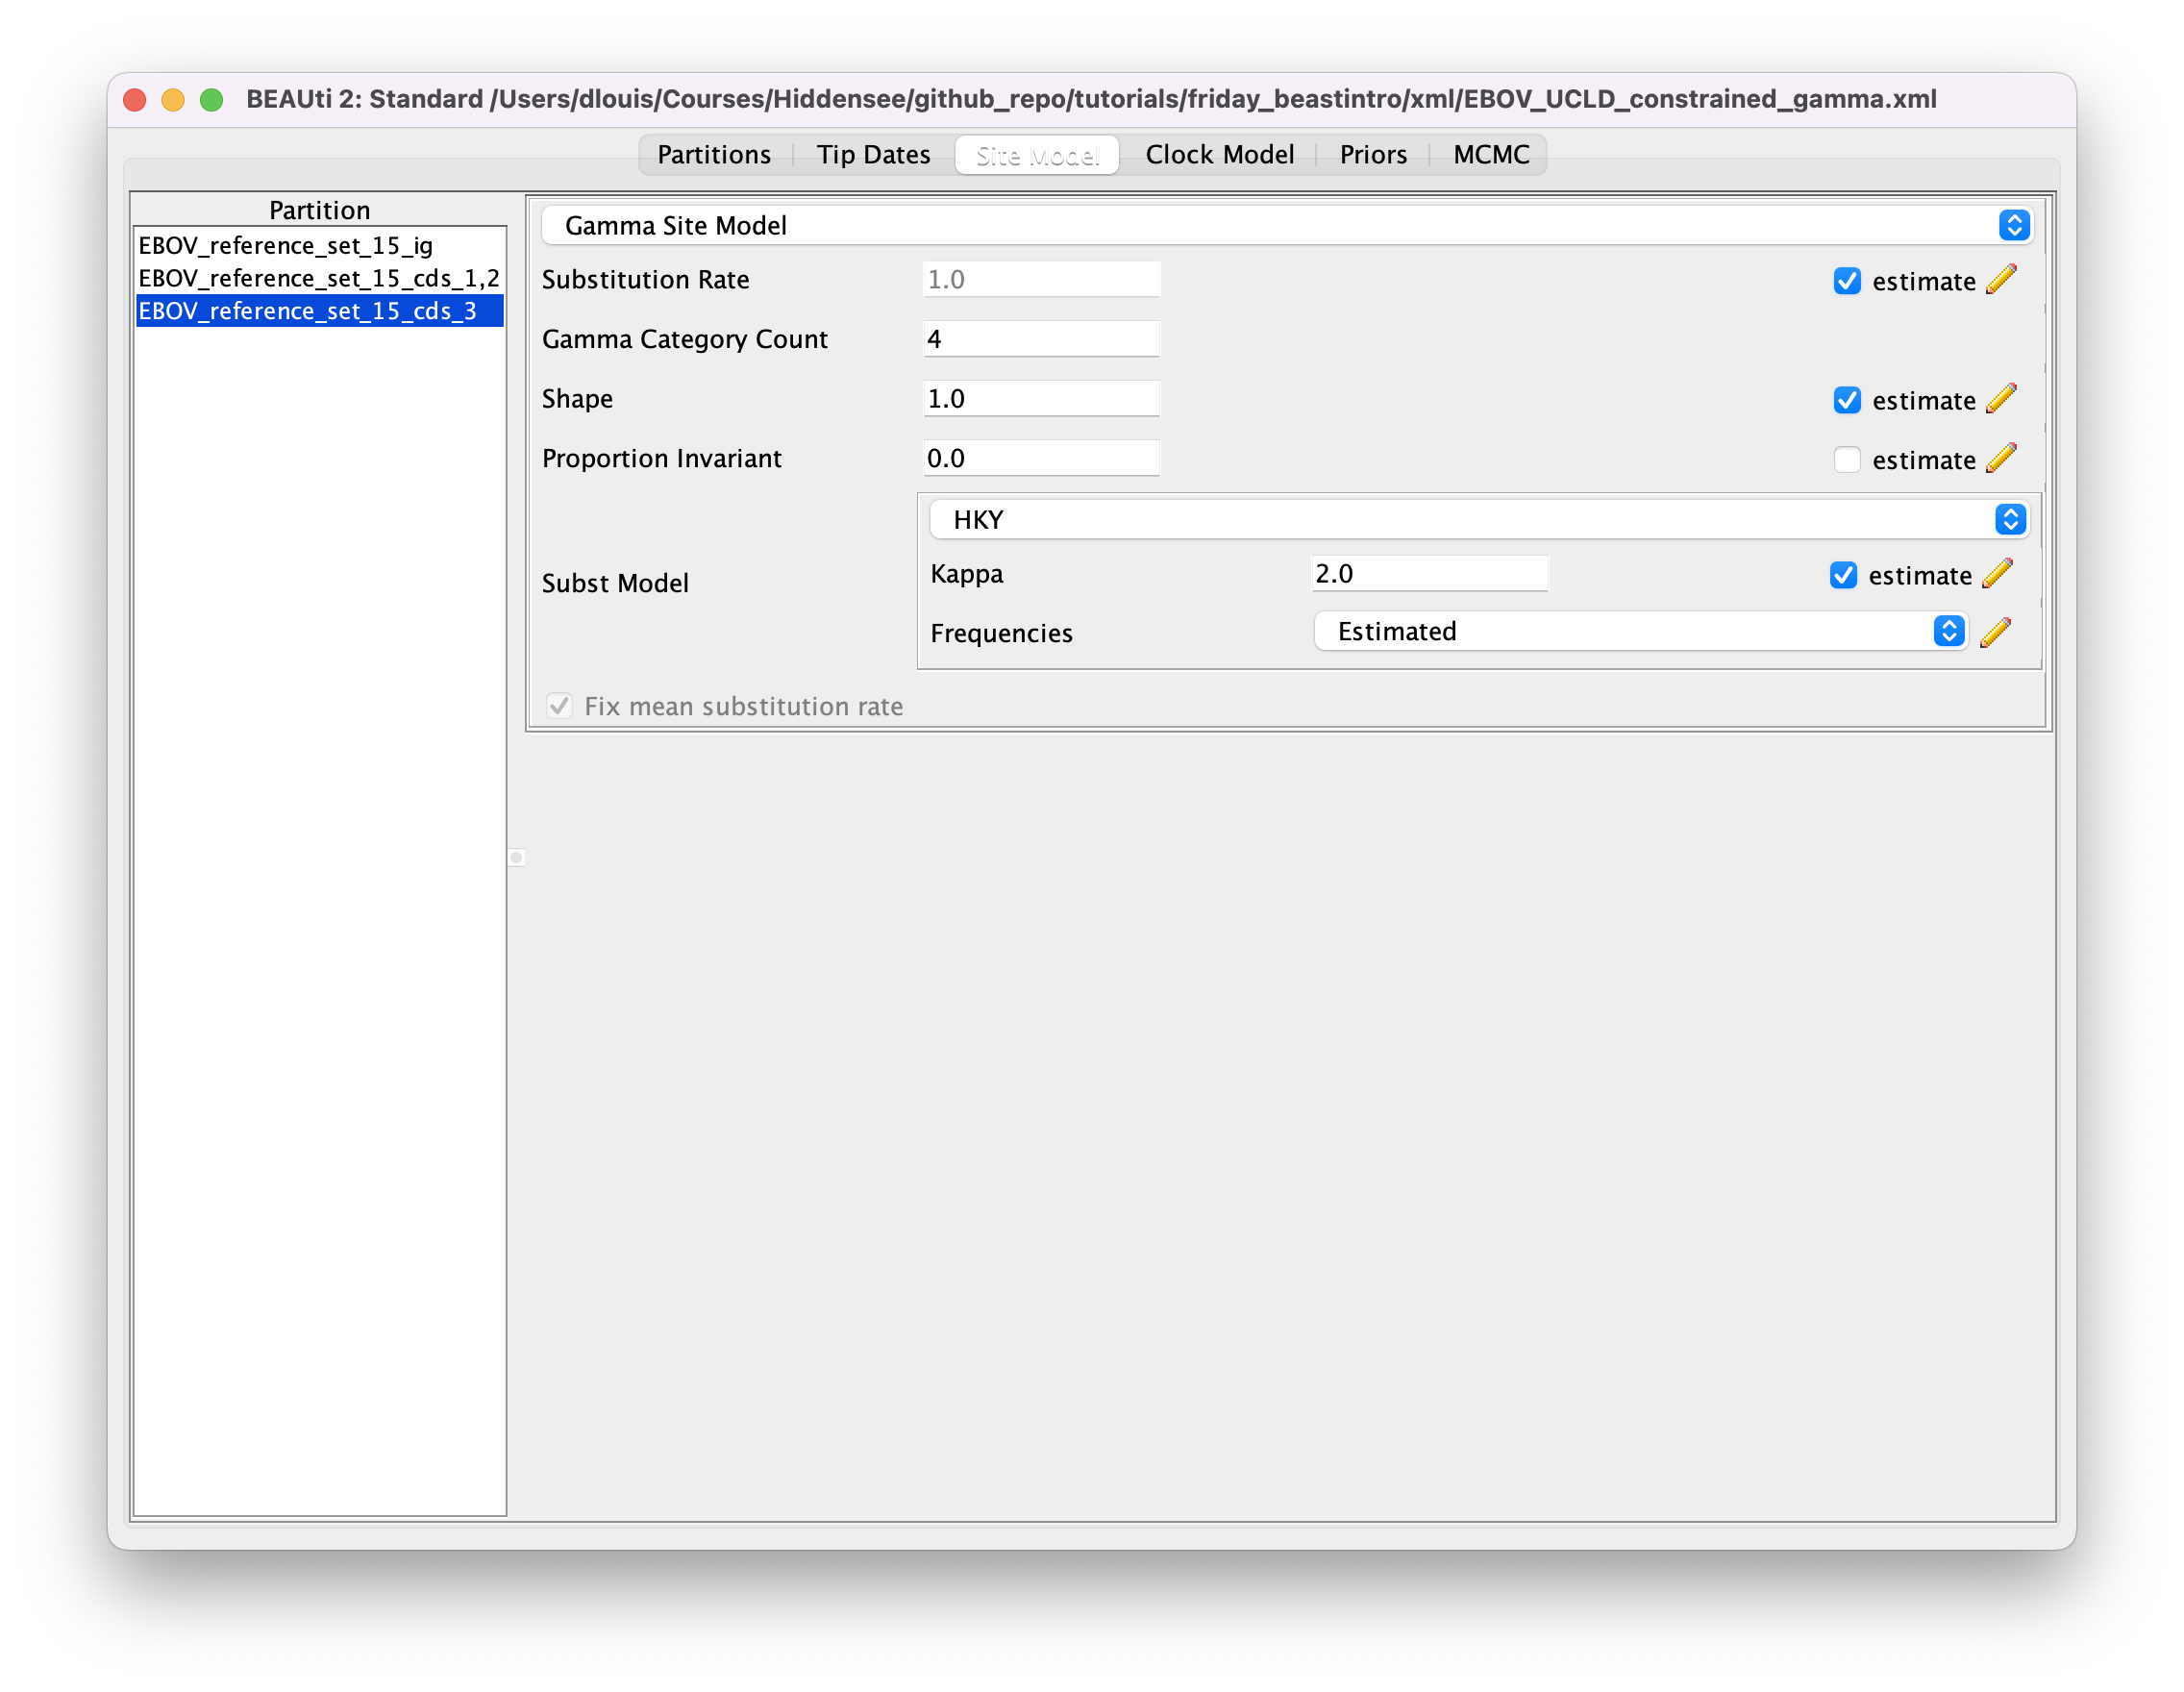
\includegraphics[max width=\textwidth, max height=0.9\textheight]{figures/gamma.png}
    \caption{The site model setup with a Gamma site model.}
    \label{fig:gamma}
\end{figure}

The site model setup should look as in Figure~\ref{fig:gamma}. No changes need to be made to the priors (we will use the default priors for the shape and frequency parameters). 
Change the log and tree file names, save the file as \lstinline!EBOV_UCLD_constrained_gamma.xml! and run the analysis
in BEAST2 (with seed 777). 

Note that this analysis is taking a lot longer to run than the previous analyses. That is because with a Gamma category
count of 4 BEAST2 needs to do approximately 4 times as many operations to calculate the likelihood. This is why we don't
usually use a lot of rate categories to discretize the Gamma distribution. In practice 4 categories allow a substantial
amount of variation while also not increasing the overhead too much. 

There is already a pre-cooked log file of this analysis that was run a lot longer
in the \lstinline!precooked_runs/! folder. Load this file into Tracer and compare it
to the earlier relaxed clock analysis without the Gamma model. 


\begin{framed}
The \textbf{Trace} tab is primarily a diagnostic tool for checking
convergence to the posterior, assessing the length of the burn-in and
whether or not the chain is mixing well. There is a good argument to be
made for this being the \emph{most important} tab in the Tracer program
and that it is the first tab users should look at.

Have a look at the individual parameter traces in the \textbf{Trace}
tab, in both the short and long log files. Can you figure out why ESS
values for some parameters are higher than others?

Do you think a burn-in of 10\% is sufficient for this analysis?

Do you think adding the Gamma model and estimating the frequencies 
added any new insights here?
\end{framed}


\begin{figure}
    \centering
    \includegraphics[max width=\textwidth, max height=0.9\textheight]{figures/tracer_good.png}
    \caption{Trace of the long run with good ESS values.}
    \label{fig:tracer_terrible}
\end{figure}



\subsection{Visualising tree posteriors
(optional)}\label{visualising-tree-posteriors-optional}

The MCC tree is one way of summarising the posterior distribution of
trees as a single tree, annotated with extra information on some nodes
to represent the uncertainty in the tree estimates. Just as summarising
the posterior distributions of a continuous parameter as a median and
credible interval throws away a lot of information (such as the shape
of the distribution) a lot of information is lost when summarising a set
of trees as an MCC tree. However, it is significantly more difficult to
visualise the set of posterior trees.

One possibility is to use the program \textbf{DensiTree}. DensiTree does
not need a summary tree (so we do not need to run TreeAnnotator prior to
using DensiTree) to be able to visualise the estimates.

\begin{framed}
Open \textbf{DensiTree}. Use \textbf{File \textgreater{} Load} then
locate and click on \lstinline!EBOV_UCLD_constrained_gamma_long.trees!.

Expand the \textbf{Show} options and check the \textbf{Consensus Trees}
checkbox.
\end{framed}

You should now see many lines corresponding to all the individual trees
sampled by the MCMC chain. You can also clearly see a pattern across
all of the posterior trees.

\begin{framed}
In order to see the support for the topology, select the
\textbf{Central} view mode.

Now expand the \textbf{Clades} menu, check the \textbf{Show clades}
checkbox and the \textbf{text} checkbox for the \textbf{Support}.
\end{framed}

The tree should look as shown in Figure \ref{fig:densitree}.

\begin{figure}
    \centering
    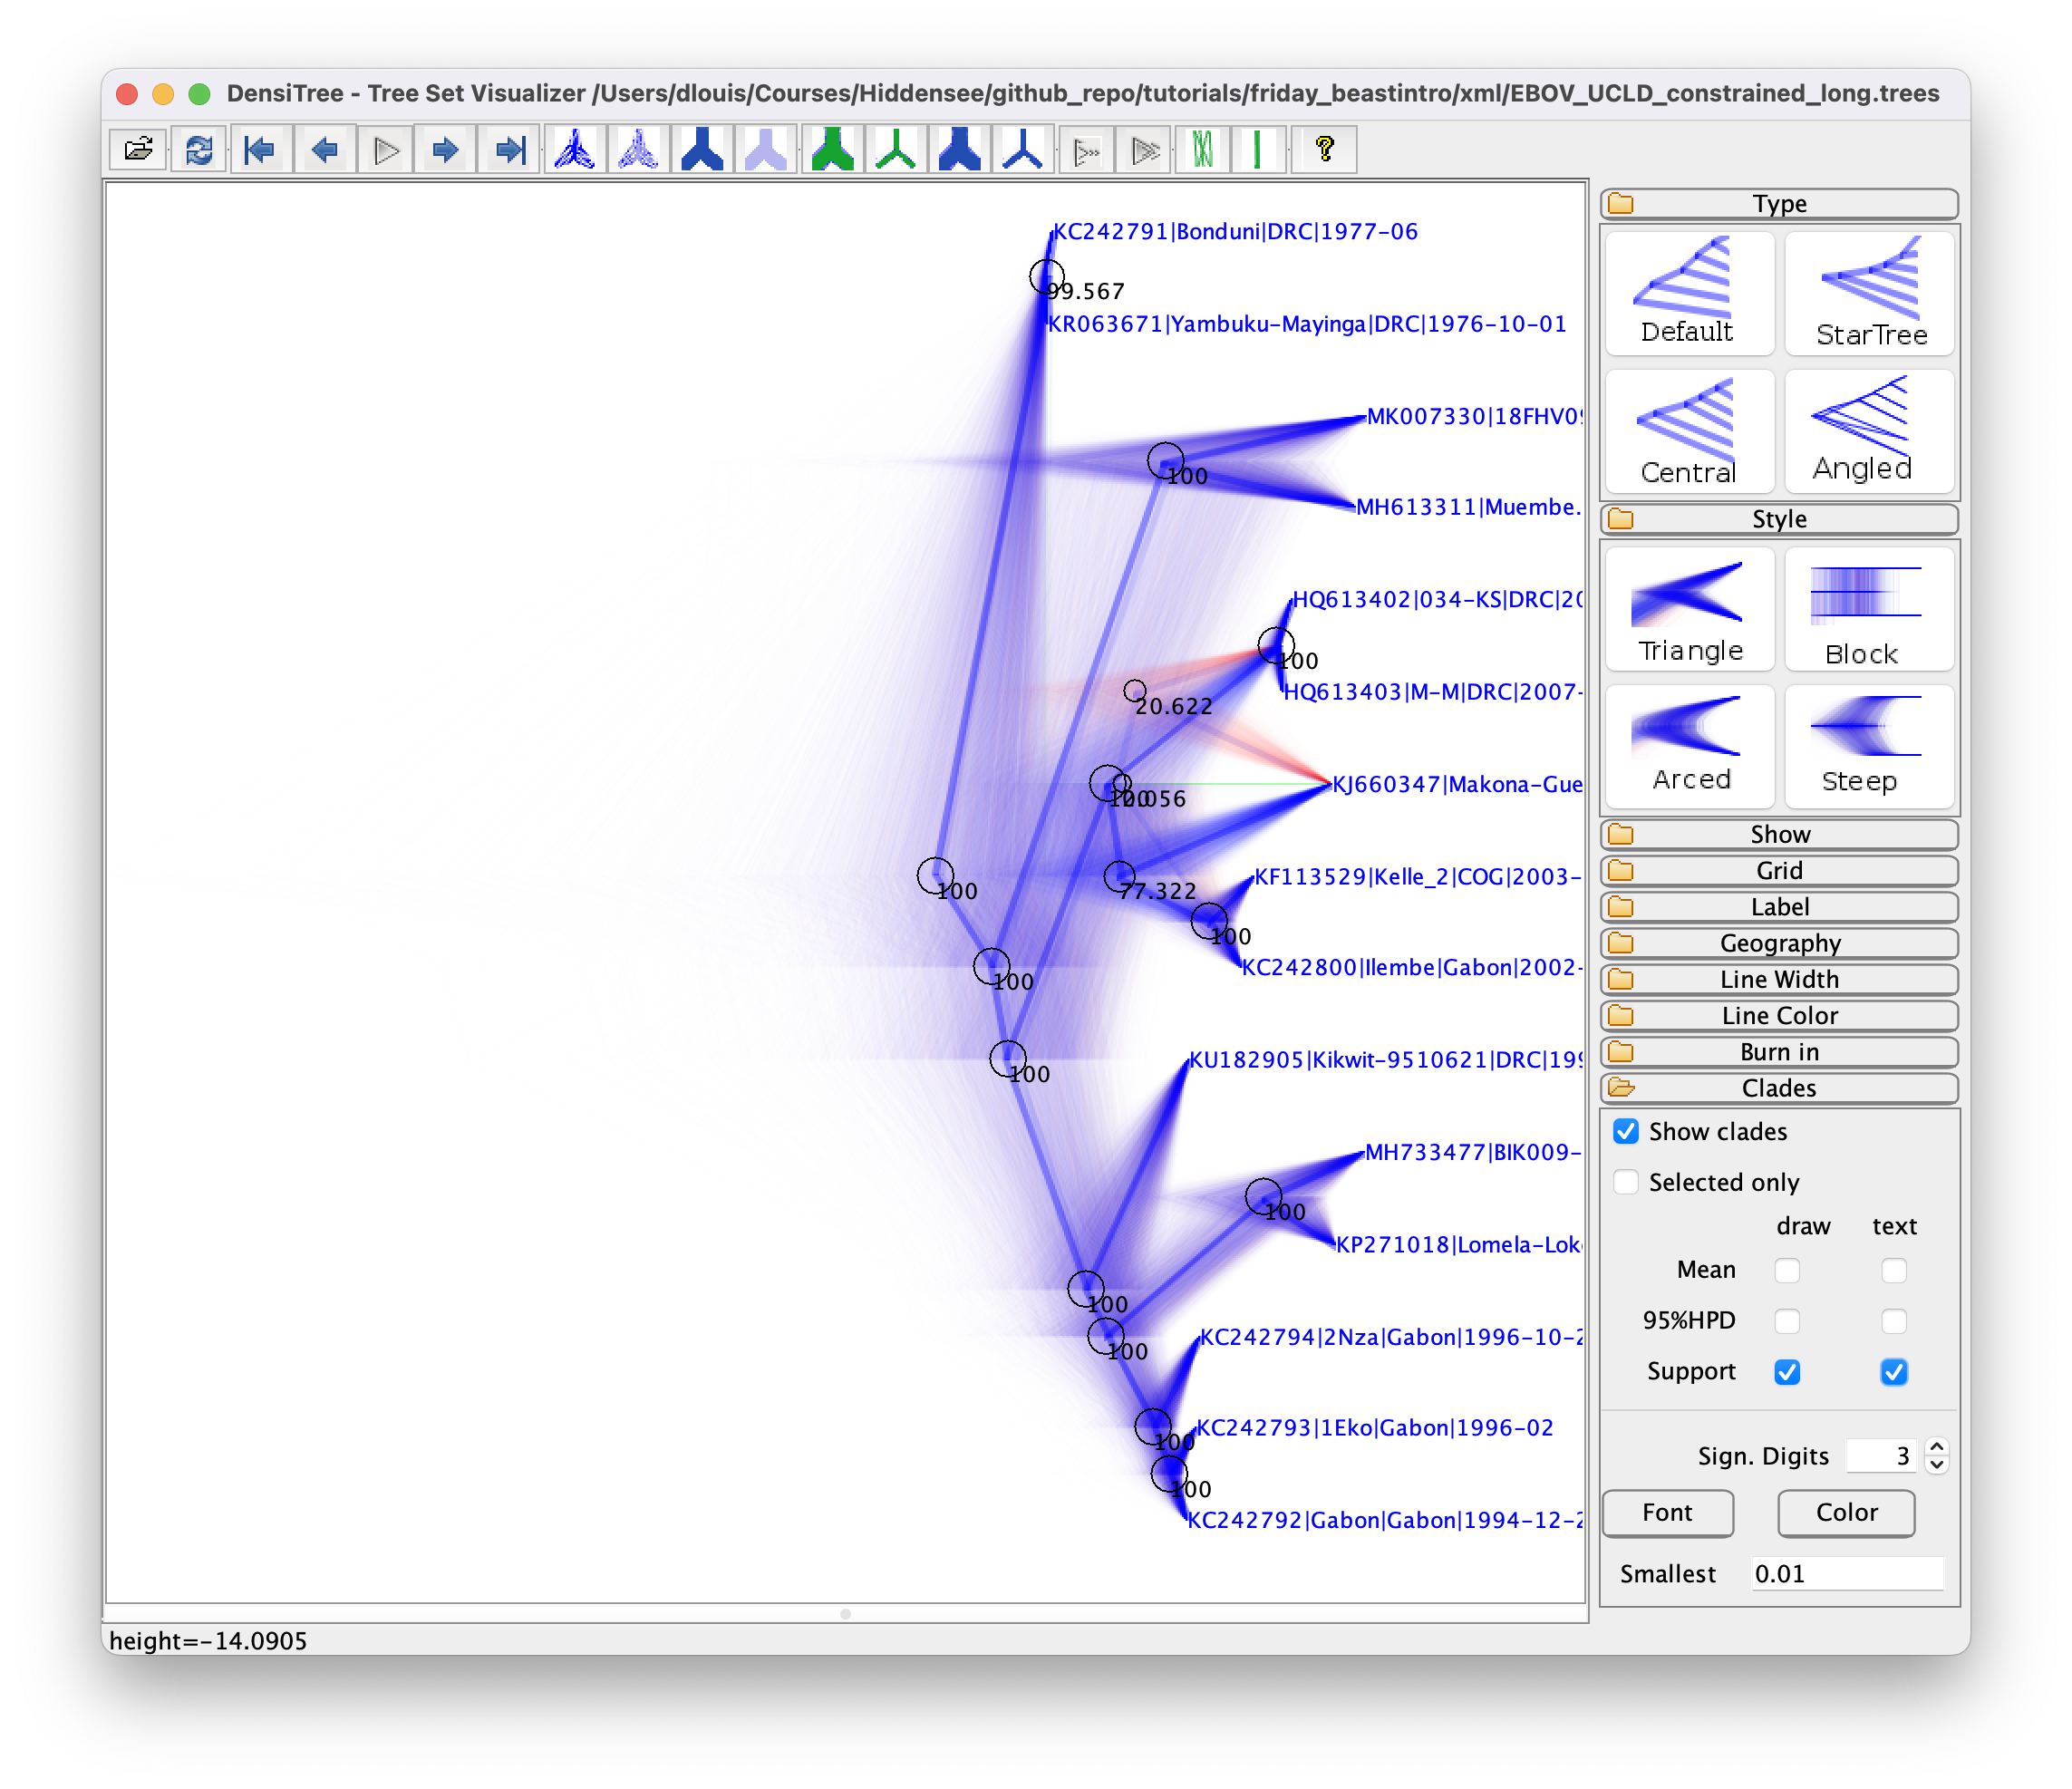
\includegraphics[max width=\textwidth, max height=0.9\textheight]{figures/densitree.png}
    \caption{DensiTree visualisation of the tree sample.}
    \label{fig:densitree}
\end{figure}

You can also view all of the different clades and their posterior
probabilities by selecting \textbf{Help \textgreater{} View clades}. In
this particular run there is little uncertainty in the tree estimate
with respect to clade grouping, as almost every clade has close to 100\% support.

\clearpage




%%%%%%%%%%%%%%%%%%%%%%%
% Tutorial disclaimer %
%%%%%%%%%%%%%%%%%%%%%%%
% Please do not change the license
% Add the author names and relevant links
% Add any other aknowledgments here
\href{http://creativecommons.org/licenses/by/4.0/}{
\includegraphics[scale=0.8]{figures/ccby.pdf}} This tutorial was written by Louis du Plessis and is licensed under a \href{http://creativecommons.org/licenses/by/4.0/}{Creative Commons Attribution 4.0 International License}. 


%%%%%%%%%%%%%%%%%%%%
% Do NOT edit this %
%%%%%%%%%%%%%%%%%%%%
Version dated: \today


%%%%%%%%%%%%%%%%
%  REFERENCES  %
%%%%%%%%%%%%%%%%

\printbibliography


\end{document}